\documentclass[a4paper]{report}  %Es un DINA4, report es el que s'adecua més a les necessitats
\usepackage [spanish,english,catalan]{babel} %last language as default
%\usepackage [OT1]{fontenc}
\usepackage [T1]{fontenc}
%\usepackage [latin1]{inputenc} 
\usepackage[utf8]{inputenc}

\usepackage{graphicx} %Per insertar imatges 

\usepackage{float} %Vull la imatge aquí! 

\usepackage{listings} %Per als llistats de codi

\usepackage{setspace} % paquete para interlineado

\usepackage{color}
\definecolor{gray97}{gray}{.97}
\definecolor{gray75}{gray}{.75}
\definecolor{gray45}{gray}{.45}

%Volen 2.5cm a dalt, 2.5cm a la dreta, 2.5cm a baix i 3cm a l'esquerra 
%\pdfpagewidth 8.5in %Height and width of the PDF page to create (i.e. size of paper you'd print on).
%\pdfpagewidth 19.7cm
%\pdfpageheight 21.0cm
%\pdfpageheight 11in
%\setlength\topmargin{0in} %Margin at top of page above all printing. Add 1 inch (so that, for example, setting \topmargin to 0.25in would produce a top margin of 1.25 inches).
\setlength\topmargin{-1.30cm}
\setlength\oddsidemargin{0.5cm}
\setlength\evensidemargin{0.5cm} 
\setlength\textheight{24.7cm}
\setlength\textwidth{15.5cm}
%\setlength\headheight{0in} %Height of the header (the header is text that appears atop all pages).
%\setlength\headsep{0in} %Distance from bottom of header to the body of text on a page.
%\setlength\textheight{7.7in} %Height and width of main text box.
%\setlength\textwidth{6.5in}
%\setlength\oddsidemargin{0in} %Left margin on odd numbered pages. Add 1 inch (as with \topmargin).
%\setlength\evensidemargin{0in} %Left margin on even numbered pages. Add 1 inch (as with \topmargin).
%\setlength\headheight{77pt} %Height of the header (the header is text that appears atop all pages).
%\setlength\headsep{0.25in} Distance from bottom of header to the body of text on a page.



\setlength\headheight{0.5cm} %Height of the header (the header is text that appears atop all pages)
\setlength\headsep{0.80cm} %Distance from bottom of header to the body of text on a page. 
 
 
\usepackage{fancyhdr}
\pagestyle{fancy}
%the number (say, 2), displayed by the macro \thechapter
%the name (in English, Chapter), displayed by the macro \chaptername
%the title, contained in the argument of \chaptermark.
\renewcommand{\chaptermark}[1]{\markboth{#1}{}}

\lhead{\footnotesize \leftmark}
\chead{}
\rhead{}
\lfoot{}
\cfoot{\thepage}
\rfoot{}
\renewcommand{\headrulewidth}{0.5pt}
\renewcommand{\footrulewidth}{0.0pt}


\lstset{ frame=Ltb,
     framerule=0pt,
     aboveskip=0.5cm,
     framextopmargin=3pt,
     framexbottommargin=3pt,
     framexleftmargin=0.4cm,
     framesep=0pt,
     rulesep=.4pt,
     backgroundcolor=\color{gray97},
     rulesepcolor=\color{black},
     %
     stringstyle=\ttfamily,
     showstringspaces = false,
	  extendedchars=true,
     basicstyle=\small\ttfamily,
     commentstyle=\color{gray45},
     keywordstyle=\bfseries,
     %
     numbers=left,
     numbersep=15pt,
     numberstyle=\tiny,
     numberfirstline = false,
     breaklines=true,
     %inputencoding=utf8x, 
     extendedchars=\true
   }
 
\lstnewenvironment{listing}[1][] % minimizar fragmentado de listados
   {\lstset{#1}\pagebreak[0]}{\pagebreak[0]}
 
\lstdefinestyle{XML}
   {language=XML
   }
 
\lstdefinestyle{PHP}
   {language=PHP
   }

\lstdefinestyle{SQL}
   {language=SQL
   }   
\lstdefinestyle{HTML}
   {language=HTML
   }

\usepackage{colortbl} %Per colorejar taules 
\usepackage{hyperref} %Per als enllaços 

\setcounter{secnumdepth}{4}
\setcounter{tocdepth}{4}

%\title{\textbf{TIMETABLE BLOCK}\\\textbf{A timetable block for Moodle\\}}
%\author{Joan Maria Talarn Espelta}
%\date{\today}

\begin{document} 

\begin{titlepage}

		\begin{figure}[H] %Here overriding the specifications of Latex good placement
		\begin{center}
		%
\includegraphics[width=14cm,keepaspectratio]{img/logodepartament.png}
		
\includegraphics{img/logodepartament.png}		
		%\caption[List caption]{Casos d'ús per l'administrador.}
		\label{fig:logodepartament}
		\end{center}
		\end{figure}

\begin{center}
{\LARGE
\textsc{\textbf{Timetable Block}}\\
\textbf{A timetable block for Moodle}\\[7cm]
}%End Large Text
\end{center}
\begin{flushleft}
\textbf{TITULACIÓ:} Enginyeria Tècnica en Informàtica de Gestió\\[5cm]
\end{flushleft}
\begin{flushright}
\textbf{AUTOR:} Joan Maria Talarn Espelta\\[1cm]
\textbf{Data:} Abril 2009\\
\end{flushright}

\end{titlepage}

%\maketitle

\begin{abstract}
\begin{onehalfspace} % tambien se puede usar onehalfspace, doublespace y singlespace
Moodle és un servidor de continguts encarat als llocs o centres educatius, i està ampliament implementat en multitud de centres.\\
La majoria d'aquests centres, però, no solament ofereixen continguts on-line sinó que Moodle els serveix com a eina de suport a les seves classes.\\
Timetable Block, está destinat a ser utilitzat en aquests centres com a eina informativa i de gestió dels grups en que cada curs està dividit i el lloc físic on es fan les classes.\\
En primer lloc, s'ofereix informació immediata del lloc on estan programades les classes i qualsevol canvi en la programació de les classes es veu reflectit a tots els usuaris que hi tenen accès.\\
I en segon lloc, serveix per oferir informació addicional als professors sobre els accessos al lloc Moodle si son efectuats amb màquines dins de l'àmbit permès i comprovar l'assistència dels alumnes.\\
Per tant, en aquest bloc seran configurables tant les hores lectives com les aules de les que disposa el centre o institució per l'elaboració de les classes.\\
\\
Resumint, aquest bloc ens ofereix les següent funcionalitats: \\
Una eina simple de gestió dels recursos físics com serien les aules on es donarien les classes. Aquesta gestió implicaria el manegament per cada aula de la seva capacitat com també si es tracta d'una aula amb ordinadors connectats en xarxa del rang d'adreces IP que tindrien les màquines ubicades en aquella aula.\\
Una eina de gestió en la que els professors poden confeccionar els horaris dels cursos que ells imparteixen. Aquesta gestió implica la gestió dels diferents grups en que es pot dividir un curs, com podrien ser els grups de classes pràctiques i els grups de classes teòriques, aixi com també l'assignació de l'aula, d'entre les disponibles en el moment de la classe.\\
Una eina informativa per als professors per poder consultar en tot moment quins són els alumnes de cada grup i desde quines màquines s'han realitzat els accessos durant les hores de classe,i així poder portar un control de l'assistència virtual.\\
I finalment una eina informativa per l'alumnat per poder consultar els horaris i la disponibilitat dels grups en els quals es divideixen els cursos als quals està matriculat.\\
\end{onehalfspace}
\end{abstract}

\begin{otherlanguage}{english}
\begin{abstract}
\begin{onehalfspace}
Moodle is a content management server used for schools and educational centers, and is widely implemented in many centers.\\
Most of these centers, however,  not only offer content online, but Moodle is used as a tool to give support to their classes.\\
Timetable Block, is intended to be used in these centers as an information and management tool of the groups in which each course can be divided and the physical place where the classes are token.\\
First, it provides immediate information on where the classes are scheduled, and any change in the classes scheduling is reflected for all users who have access.\\
And secondly, can be used to provide additional information to the teachers about Moodle site accesses and if this accesses are made with machines allowed in the class environment allowed and check the students attendance.\\
Therefore, in this block can be configured hours and classrooms available in the center or institution for the development of classes.\\
\\
In short, this block offers the following features: \\
A simple tool for managing the physical resources as the classroom where he would give lessons. This management would manage each of their classroom as well as in the case of a classroom with networked computers, the range of the IP addresses of the machines would be located in the classroom.\\
A management tool for the teachers to do the timetables of the courses they teach. This management involves the management of different groups that can divide a course, such as groups of practical classes and groups of theorical classes, as well as the allocation of the classroom, from those available at the time of the class .\\
An informative tool for teachers to consult at any time who are the students in each group and from which machines have made access during school hours, so we can keep track of virtual attendance.\\
And finally an informational tool for students to check timetables and availability of the groups that are divided the courses to which it is registered.\\
\end{onehalfspace} 
\end{abstract}
\end{otherlanguage}

\begin{otherlanguage}{spanish}
\begin{abstract}
\begin{onehalfspace}
Moodle es un servidor de contenidos encarado a los lugares o centros educativos, y está ampliamente implementado en multitud de centros.\\
La mayoría de estos centros, sin embargo, no sólo ofrecen contenidos on-line sino que Moodle les sirve como herramienta de apoyo a sus clases.\\
Timetable Block, está destinado a ser utilizado en estos centros como herramienta informativa y de gestión de los grupos en que cada curso está dividido y el lugar físico donde se realizan las clases.\\
En primer lugar, se ofrece información inmediata del lugar donde están programadas las clases y cualquier cambio en la programación de las clases se ve reflejado para todos los usuarios que tengan acceso.\\
Y en segundo lugar, sirve para ofrecer información adicional a los profesores sobre los accesos al sitio Moodle y si son efectuados con máquinas dentro del ámbito permitido y poder comprobar la asistencia de los alumnos.\\
Por tanto, en este bloque serán configurables tanto las horas lectivas como las aulas de las que dispone el centro o institución para la elaboración de las clases.\\
\\
Resumiendo, este bloque nos ofrece las siguientes funcionalidades: \\
Una herramienta simple de gestión de los recursos físicos como serían las aulas donde se darían las clases. Esta gestión implicaría el manejo para cada aula de su capacidad así como también, si se trata de una aula con ordenadores conectados en red, del rango de direcciones IP que tendrían las máquinas ubicadas en esa aula.\\
Una herramienta de gestión en la que los profesores pueden confeccionar los horarios de los cursos que ellos imparten. Esta gestión implica la gestión de los diferentes grupos en que se puede dividir un curso, como podrían ser los grupos de clases prácticas y los grupos de clases teóricas, así como también la asignación del aula, de entre las disponibles en el momento de la clase.\\
Una herramienta informativa para los profesores para poder consultar en todo momento cuáles son los alumnos de cada grupo y desde qué máquinas se han realizado los accesos durante las horas de clase, y así poder llevar un control de la asistencia virtual.\\
Y finalmente una herramienta informativa para el alumnado para poder consultar los horarios y la disponibilidad de los grupos en los que se dividen los cursos a los que está matriculado.\\
Por tanto, en este bloque serán configurables tanto las horas lectivas como las aulas de las que dispone el centro o institución para la elaboración de las clases.\\
\end{onehalfspace} 
\end{abstract}
\end{otherlanguage}
\tableofcontents



\chapter{Introducció}

\section{Què és un CMS}
CMS són les sigles de Content Management System, en català, Sistema de Gestió de Continguts.
Els gestors de continguts són sistemes per mantenir i actualitzar webs de manera fàcil. Normalment funcionen a través del mateix web, i a vegades a través d'aplicacions específiques. Els sistemes de gestió de continguts que s'han extès més són els que tenen origen al programari lliure.
Gràcies a llicències com la GNU GPL, el codi font és públic i qualsevol és lliure de modificar-lo, copiar-lo o distribuir-lo. En conseqüència, qualsevol programador té accés al codi i pot co\l.laborar lliurement en tots aquests projectes, fent possible el seu desenvolupament i extensió.
Els CMS més coneguts són programats amb llenguatges interpretats tals com PHP, Perl, Ruby, pel que fa a programari lliure, i amb ASP o JSP, pel que fa al privatiu.
Els objectius dels CMS són molt variats: intranets, blogs, portals de notícies, webs d'empreses...

\section{Moodle}
\subsection{Què és}
Moodle és un paquet de programari per a la creació de cursos i llocs web basats en Internet. És un projecte en desenvolupament dissenyat per a donar suport a un marc d'educació constructivista social. 
Moodle es distribueix de manera gratuïta com a programari lliure (Open Source) (sota la Llicència Pública GNU). Bàsicament això vol dir que Moodle té drets d'autor (copyright), però que teniu algunes llibertats. Podeu copiar, utilitzar i modificar Moodle sempre que accepteu: proporcionar el codi font als altres, no modificar o eliminar la llicència original i els drets d'autor, i aplicar aquesta mateixa llicència a qualsevol treball que en derivi. Llegiu la llicència per a més detalls i contacteu amb l'amo dels drets d'autor directament si teniu alguna pregunta. 
Moodle pot funcionar en qualsevol ordinador on pugui córrer PHP i suporta diversos tipus de base de dades (en especial MySQL). 
La paraula Moodle era al principi un acrònim de Modular Object-Oriented Dynamic Learning Environment (Entorn d'Aprenentatge Dinàmic Orientat a Objectes i Modular), la qual cosa resulta fonamentalment útil per a programadors i teòrics de l'educació. També és un verb que descriu el procés de deambular peresosament a través d'alguna cosa i fer les coses quan se t'acut fer-les, un plaent nyap que sovint et porta a a visió i a la creativitat. Totes dues accepcions s'apliquen a la manera en què es va desenvolupar Moodle i a la manera en què un estudiant o podria aproximar-se a l'estudi o ensenyament d'un curs en línia. Tot aquell qui utilitza Moodle és un Moodler. 
El projecte fou iniciat, i és mantingut, per l'australià Martin Dougiamas. Però ha aconseguit reunir una gran comunitat internacional d'usuaris, programadors, desenvolupadors i traductors de tal forma que actualment té 75.000 usuaris registrats i està traduït a 70 llengües, inclòs el català.
La clau del seu èxit rau en la facilitat d'insta\l.lació (només necessita un servidor php i una base de dades com MySQL), de configuració, creació de cursos i manteniment del lloc. Està construït sota una òptica de construcció del coneixement basat en el diàleg entre els participants, el constructivisme social. Per això és tan fàcil crear-hi fòrums. Tot i això accepta molts altres tipus d'activitats didàctiques: qüestionaris, lliçons, tasques, wikis, xats, etc.
\subsection{Filosofia}
 El diseny i desenvolupament de Moodle es basen en la idea de la pedagogia construccionista social. Aquesta filosofia radica en la cooperació en grup i en la idea de que el coneixement es pot crear o construir.
Com a curiositat, cal fer menció que Moodle és la primera comunitat Open Source no formada íntegrament per informàtics, sinó que també participen pedagogs i altra gent relacionada amb l'ensenyament.
\subsection{Característiques}
Promou la pedagogia constructivista social.\\
Es poden fer les classes 100\% on-line.\\
Té una interfície senzilla, lleugera i molt intuïtiva.\\
Insta\l.lable en qualsevol plataforma que suporti PHP (només requereix l'existència d'una base de dades).\\
Ofereix un llistat dels cursos amb descripcions i la posibiliat d'entrar-hi com a usuari convidat.\\
Seguretat ben sòlida, els formularis es revisen, les cookies s'encripten.\\
El tema de la interfície és altament personalitzable.\\
Els paquets d'idioma permeten localitzar a qualsevol idioma per complet (70 idiomes).\\
Inclou diversos mòduls per a tallers, fòrums, consultes, xats, etc.\\
Alta Disponibilitat.\\
Escalabilitat.\\
Fàcil ús.\\
Interoperable.\\
Estable.\\
Segur.\\
\subsection{Com funciona}
\subsubsection{Requisits}
Moodle està preparat per al Linux fent servir Apache, MySQL PHP (sovint es reconeix amb el nom LAMP el conjunt d'aquests quatre components), però també s'ha provat als sistemes operatius Windows XP/2000/2003 (WAMP), Solaris 10 (Sparc i x64), Mac OS X i Netware 6. També es pot treballar amb els servidors de dades PostgreSQL, Oracle i Microsoft SQL.\\
Els requisits per al Moodle són els següents:
\begin{itemize}
   \item Maquinari (si utilitzeu un servidor propi):
   \begin{itemize}
   	\item Espai de disc: 160Mb lliures (com a mínim). Us caldrà més espai lliure per desar-hi els materials d'ensenyament. 
		\item Memòria: 256Mb (mínim), 1Gb (recomanat). Com a norma general, Moodle suportarà 50 usuaris $"$concurrents$"$ per cada gigabit de memòria RAM, però això pot variar en funció del maquinari específic i la combinació de programes. 
	\end{itemize}
	\item Programari: 
	\begin{itemize}
		\item Servidor web. La majoria de gent utilitza Apache, però el Moodle hauria de treballar correctament en qualsevol servidor web que suporti PHP, com ara IIS a les plataformes Windows. PHP imposa unes necessitats segons la versió del servidor web, que són complexes, i normalment el consell general que es pot donar és que es faci servir la versió més recent possible del servidor web escollit. 
		\item El llenguatge d'escripts PHP. (Penseu que hi ha hagut millores havent insta\l.lat el Moodle amb el programari PHP-Accelerator). De moment hi ha dues versions de PHP accessibles: PHP4 i PHP5. 
			\begin{itemize}
			\item Per al Moodle 1.4 o posterior, es suporten aquestes versions: PHP4 (versió 4.1.0 o posterior) o PHP5 (versió 5.1.0 o posterior). 
			\item Per al Moodle 1.6 o posterior, es suporten aquestes versions: PHP4 (versió 4.3.0 o posterior) o PHP5 (versió 5.1.0 o posterior). 
			\item Les versions futures del Moodle 2.0 o posteriors ja no acceptaran PHP4 i necessitaran PHP5 o posteriors). 
			\end{itemize}
		\item Un servidor de base de dades: MySQL i PostgreSQL estan completament suportats i recomanats. El suport per a Microsoft SQL Server i Oracle s'ha afegit al Moodle 1.7. MySQL és el que tria molta gent perquè és molt popular, però hi ha alguns arguments a favor de PostgreSQL, especialment si heu planejat un desenvolupament molt extens. 
			\begin{itemize}
			\item Per al Moodle 1.5 o posteriors, MySQL (versió 3.23 o posterior) o PostgreSQL (7.4 o posterior). 
			\item Per al Moodle 1.6 o posteriors, MySQL (versió 4.1.12 o posterior) o PostgreSQL (7.4 o posterior). 
			\item \textbf{Notes:} Per al Moodle 1.6 o posterior. Si utilitzeu codis de llenguatge només llatins, podeu utilitzar MySQL 4.1.12. Si utilitzeu codis no-llatins us caldrà MySQL 4.1.16 o posterior. De moment el paràmetre $"$strict mode$"$ de MySQL ha de ser OFF (establert a $"$$"$ o $"$MYSQL40$"$) al fitxer de configuració de MySQL. La versió mínima de PostgreSQL és 7.4 i s'utilitzen molt la 8.0 i la 8.1. La versió mínima de Microsoft SQL Server és la 2005 (versió 9). També hi ha hagut intents amb SQL Server Express 2005. 
			\end{itemize}
 	\end{itemize}
 \end{itemize}
\begin{itemize}
	\item Requeriments addicionals de PHP
		\begin{itemize}
		\item Paràmetres de PHP
			\begin{itemize}
			\item El Safe mode ha d'estar en OFF (comproveu-ho al fitxer php.ini o al fitxer de configuració d'Apache).
			\item El paràmetre memory\_limit ha de ser com a mínim 16M (es recomana que sigui 32M per al Moodle 1.7 o posterior).
			\item El paràmetre de PHP session.save\_handlerha d'establir-se a files.
			\end{itemize}
		\item Extensions de PHP i llibreries
			\begin{itemize}
			\item L'extensió mbstring es necessita per controlar cadenes multi-byte. 
			\item L'extensió iconv també es necessita per al Moodle 1.6 o posterior. 
			\item Les llibreries i extensions GD library i FreeType 2 també es necessiten per poder mostrar els gràfics dinàmics que es fan a les pàgines de registres. 
			\item L'extensió mysql cal si utilitzeu la base de dades MySQL. Fixeu-vos que en algunes distribucions de Linux (especialment Red Hat) es tracta d'una insta\l.lació opcional. 
			\item L'extensió pgsql cal si utilitzeu la base de dades PostgreSQL. 
			\item L'extensió zlib cal per afegir la funcionalitat zip de compressió i descompressió. 
			\item Pot ser que calguin altres extensions PHP per poder suportar altres funcionalitats del Moodle, especialment les d'autenticació i/o enrolament (p.ex. l'extensió LDAP per a l'autenticació LDAP i l'extensió de sockets per al servidor de Xat) 
			\end{itemize}
		\end{itemize}
\end{itemize}
\subsubsection{Usuaris}
A més del maquinari i del programari, també heu de pensar en la capacitat de la insta\l.lació Moodle en funció del nombre d'usuaris que ha de poder suportar. Cal tenir en compte dos números: 
\begin{itemize}
\item \textbf{Usuaris de navegació:} el nombre màxim d'usuaris que podran navegar pel lloc Moodle. És el nombre d'ordinadors del centre o del curs (el més alt). 
\item \textbf{Usuaris concurrents de la base de dades:} el nombre màxim d'usuaris concurrents de la base de dades (en activitats Moodle com ara qüestionaris). És el nombre d'usuaris que utilitzaran el Moodle simultàniament. En una institució educativa, calculeu amb els horaris i llistes en mà. 
\end{itemize}
Quan sapigueu aquestes quantitats, podeu deduir el model de la insta\l.lació. El nombre exacte d'usuaris depèn de la combinació maquinari/programari/xarxa. Normalment la quantitat de memòria (RAM) insta\l.lada és el factor decisiu, però un processador més ràpid també contribuirà a reduir el temps de càrrega de les pàgines. 
La regla general per a un servidor sol és que el nombre màxim aproximat d'usuaris = RAM (en Gb) * 50 i que el nombre màxim aproximat d'usuaris de navegació = Màxim aproximat d'usuaris concurrents * 5. Per exemple, una universitat amb un total de 500 ordinadors al campus i 100 usuaris concurrents, necessitarà aproximadament 2Gb de RAM en un servidor per donar-hi suport. 
\subsubsection{Estructura de directoris de Moodle}
Un resum dels continguts del directori Moodle, per orientar-vos: 
\begin{itemize}
\item config.php - conté paràmetres bàsics. El fitxer no es descarrega amb el moodle, es crea. 
\item install.php - l'escript que s'engega per crear el fitxer config.php 
\item version.php - defineix la versió en curs del codi Moodle 
\item index.php - la pàgina principal del lloc 
\item admin/ - codi per administrar tot el servei 
\item auth/ - mòduls dels connector per a autenticació d'usuaris 
\item blocks/ - mòduls dels connectors per als blocs laterals de la majoria de pàgines 
\item calendar/ - tot el codi per al maneig i la visualització de calendaris 
\item course/ - codi per a mostrar i gestionar cursos 
\item doc/ - documentació d'ajuda per al Moodle (per exemple, aquesta pàgina) 
\item files/ - codi per a mostrar i gestionar fitxers penjats al lloc 
\item lang/ - textos en llengües diverses, un directori per a cada llengua 
\item lib/ - co\l.leccions de tot el codi Moodle 
\item login/ - codi per a controlar l'entrada al lloc i creació de comptes d'usuari 
\item mod/ - tot el codi dels mòduls de gestió de cursos 
\item pix/ - els gràfics genèrics del lloc 
\item theme/ - paquets de temes/pells per a canviar l'aspecte del lloc. 
\item user/ - codi per al maneig, dades i llistes d'usuaris 
\end{itemize}
\subsubsection{Creació d'una base de dades buida}
Caldrà que creeu una base de dades buida (per exemple, $"$moodle$"$) al sistema de base de dades, i un usuari especial (per exemple, $"$usuari\_moodle$"$) que tingui accés a aquesta base de dades (aquesta i prou). Podeu fer servir l'usuari $"$root$"$ si treballeu en un servidor de prova, però no és gens recomanable en un sistema de producció: si un hacker arriba a descobrir el mot de pas tot el sistema de base de dades estarà en perill, no només una base de dades.
\subsubsection{Creació del directori de dades (moodledata)}
Moodle també necessitarà espai al disc dur del servidor per guardar-hi els fitxers penjats, com ara documents de curs i fotografies d'usuaris. L'insta\l.lador del Moodle intentarà crear-vos el directori però si no pot l'haureu de crear manualment. 
\subsubsection{Creació d'un curs}
Quan el Moodle treballi correctament, podeu crear un curs per començar.\\
Trieu $"$Afegir un curs$"$ des de la pàgina d'Administració (o des dels vincles d'administració de cursos de la pàgina principal).\\ 
Empleneu el formulari, amb una atenció especial quant al format de curs. No cal que us preocupeu excessivament pels detalls en aquest moment, perquè es pot canviar tot més endavant. Fixeu-vos que les icones grogues que hi ha pertot proporcionen ajuda contextual sobre qualsevol aspecte.\\ 
Feu clic a $"$Desa els canvis$"$, i arribareu a un altre formulari on podreu assignar professorat al curs. Només podreu afegir-hi comptes d'usuari existents - si voleu crear comptes de professorat, demaneu a cada professor que es creï el seu compte personal (vegeu la pàgina d'entrada), o creeu-ne un a través dels vincles $"$Usuaris$"$, $"$Afegeix usuaris$"$ de la pàgina d'Administració.\\
En acabar, el curs ja està a punt de solfa, i és accessible al vincle $"$Cursos$"$ de la pàgina principal.\\ 
\subsubsection{Fent un nou plug-in}
La M de Moodle ve de modular, i la forma més fàcil i més mantenible d'afegir noves funcionalitats a Moodle és usant un dels molts plugins de les API. Hi ha molts tipus de plugins que pots escriure: 
\begin{itemize}
\item Activity modules 
\item Admin reports 
\item Assignment types 
\item Authentication plugins 
\item Blocks 
\item Course formats 
\item Course reports 
\item Database fields 
\item Database presets 
\item Enrolment plugins 
\item Filters 
\item Grade export/import 
\item Grade report 
\item Question engine 
\item Question import/export formats 
\item Quiz reports 
\item Resource types 
\item SSO plugins 
\end{itemize}
Els tres tipus de plugins més utilitzats i en els que la comunitat Moodle co\l.labora amb més aportacions són els que a continuació es defineixen breument: Mòduls d'activitat, Recursos i Blocs.
\subsubsection{Moduls d'activitat}
\begin{figure}[H] %Here overriding the specifications of Latex good placement
\begin{flushleft}
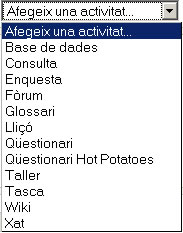
\includegraphics{img/MoodleActivitat.jpg}
\caption[List caption]{Llista de mòduls d'activitat per afegir.}
\label{fig:MoodleActivitat}
\end{flushleft}
\end{figure}
Moodle disposa d'activitats d'aprenentatge diverses que podeu afegir als vostres cursos (Figura ~\ref{fig:MoodleActivitat}).\\
La comunicació i la co\l.laboració entre els estudiants es pot produir utilitzant els xats i els fòrums. Els missatges permeten converses bidireccionals entre dos participants d'un curs. També poden treballat de manera co\l.laborativa editant de manera conjunta un wiki, una manera exce\l.lent per tal que els estudiants treballin plegats fent un projecte conjunt.\\ 
Les consultes ens permeten recollir l'opinió dels participants sobre un tema concret. També podem crear glossaris de paraules o termes clau i fins i tot permetre que els estudiants creïn les entrades (i avaluar-les). Les bases de dades, disponibles a partir de la versió 1.6, també es poden utilitzar amb aquest objectiu.\\
Els estudiants ens poden trametre els seus treballs mitjançant les tasques, que poden escriure directament en línia o bé mitjançant un fitxer que prèviament han elaborat. Els tallers permeten també la tramesa de treballs que són, a més, revisats entre els estudiants. Els qüestionaris disposen de diferents tipus de preguntes (opció múltiple, aparellament,...) amb correcció automàtica. També podem incloure activitats que haguem elaborat amb el programa HotPotatoes i integrar les qualificacions que l'estudiant obté a la seva taula de qualificacions del curs.\\ 
Les enquestes ja vénen predefinides, i poden ser útils per a convidar a la reflexió i conèixer la concepció de l'aprenentatge dels estudiants.\\ 
Però, a més, hi ha tot un seguit d'activitats no estàndard que no es troben al programa oficial de Moodle però que es poden insta\l.lar fàcilment. Entre elles podem destacar les activitats JClic o el mòdul de Quaderns Virtuals.\\ 
Aquests són amb molt els mòduls més importants, i es troben al directori $"$mod$"$. Per defecte hi ha set mòduls: Tasca, Consulta, Fòrum, Glossari, Qüestionari, Recurs i Enquesta. Cada mòdul està en un subdirectori separat i consisteix amb els següents elements obligatoris (més els scripts extra que són únics per a cada mòdul): \\
\begin{itemize}
\item mod.html: un formulari per establir o actualitzar una instància d'aquest mòdul 
\item version.php: defineix alguna meta-informació i proporciona codi d'actualització 
\item icon.gif: una icona de 16x16 per al mòdul 
\item db/: bolcats SQL de totes les taules i dades requerides de una base de dades (per a cada tipus de base de dades) 
\item index.php: una pàgina per representar la llista de totes les instàncies en un curs 
\item view.php: una pàgina per veure una instància en particular 
\item lib.php: qualsevol/totes les funcions definides per al mòdul haurien d'ésser aqui. 
\end{itemize}
Si el mòdul es diu $"$andromina$"$, llavors les funcions requerides inclouen: 
\begin{itemize}
\item andromina\_add\_instance() - codi per afegir una nova instància d'andromina 
\item andromina\_update\_instance() - codi per actualitzar una instància existent 
\item andromina\_delete\_instance() - codi per esborrar una instància 
\item andromina\_user\_outline() - donada una instància, retorna un resum d'na contribució d'un usuari 
\item andromina\_user\_complete() - donada una instància, imprimeix detalls sobre la contibució d'un usuari 
\end{itemize}
Altres funcions interessants però no obligatòries són: 
\begin{itemize}
\item andromina\_delete\_course() - per esborrar tot el que sigui necessàr després d'esborrar totes les instàncies d'un curs 
\item andromina\_process\_options() - per pre-processar la informació dels ajustaments de la instància 
\end{itemize}
Per evitar possibles conflictes, qualsevol de les funcions d'un mòdul haurà de ser nombrada començant amb andromina\_ (el nom del mòdul més un guió baix) i qualsevol constant que definexi vostè haurà de començar amb ANDROMINA\_ 
\begin{itemize}
\item config.html - (opcional) un formulari per ajustar les preferències globals del mòdul 
\end{itemize}
Finalment, cada mòdul tindrà alguns fitxers d'idioma que contenen cadenes per aquest mòdul. Llegeixi més avall.\\ 
IMPORTANT: Al crear un nou mòdul, el nom del mateix haurà de ser una paraula senzilla, amb anglès, que no inclogui números o altres caràcters especials. També haurà d'assegurar-se de que el seu mòdul proporciona suport per algunes característiques com grups, metacursos i copies de seguretat i restauració.\\
\subsubsection{Recursos}
\begin{figure}[H] %Here overriding the specifications of Latex good placement
\begin{flushleft}
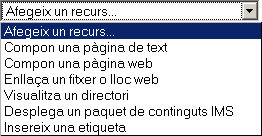
\includegraphics{img/MoodleRecurs.png}
\caption[List caption]{Llista de recursos disponibles.} 
\label{fig:MoodleRecurs}
\end{flushleft}
\end{figure}
Moodle disposa de diversos recursos que ens permeten posar qualsevol tipus de contingut en format digital a l'abast dels estudiants. Per tal d'afegir-los, amb l'edició activada, hem de seleccionar l'opció corresponent del menú (Figura ~\ref{fig:MoodleRecurs}) $"$Afegeix un recurs$"$. 
Una Pàgina de text és un recurs senzill que consisteix en una pàgina escrita en text sense format (en principi, tot i que accepta etiquetes html). Les pàgines de text són molt ràpides de fer i, tot i que no permeten donar format al text d'una manera senzilla, poden ser una bona opció per a escriure informacions curtes o instruccions breus. Si la informació que voleu donar als estudiants requereix un cert format del text amb títols, taules, imatges,... és millor que utilitzeu el recurs Composa una pàgina web, que posarà al vostre abanst un editor del tipus WYSIWYG. 
Els recursos poden tenir formats molt diversos. En aquest cas hem d'utilitzar l'opció Enllaçar un fitxer o lloc web o bé posar a l'abast dels estudiants els fitxers que hem pujat a un directori del curs mitjançant el recurs Visualitza un directori. Si disposeu d'un paquet de contingut IMS podeu utilitzar el recurs Desplega un paquet de contingut IMS. 
Les etiquetes poden ser molt útils per a mostrar informació o instruccions. També ens permeten afegir imatges i altres fitxers multimèdia a les diferents seccions del curs de manera que siguin visibles directament a la pàgina principal del curs. 
\subsubsection{Blocs}
\begin{figure}[H] %Here overriding the specifications of Latex good placement
\begin{flushleft}
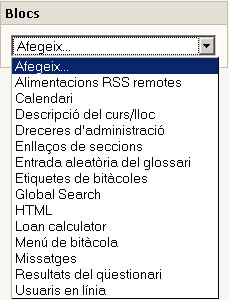
\includegraphics{img/MoodleBloc.jpg}
\caption[List caption]{Llista de blocs disponibles per ser afegits.} 
\label{fig:MoodleBloc} 
\end{flushleft}
\end{figure}
Les pàgines principals d'un curs contenen, generalment, blocs a les bandes esquerra i dreta, amb una columna central que mostra els continguts del curs. Amb l'edició activada es poden afegir, esborrar o amagar blocs, moure'ls amunt i avall i d'esquerra a dreta o vice-versa. La imatge mostra els blocs que podem afegir al curs: $"$Usuaris en línia$"$, $"$Missatges$"$, $"$Calendari$"$,... (Figura ~\ref{fig:MoodleBloc})
Una llista de més de 16 tipus diferents de blocs pot proveir informació o funcionalitats addicionals per als professors i estudiants. A la dreta es mostren els blocs estàndard que venen amb Moodle. Hi ha molts més blocs no estàndard desenvolupats per Moodlers que un administrador pot insta\l.lar i afegir a aquesta llista. 
Un professor amb drets d'editor tindrà també un bloc d'administració. Aquest bloc té submenús per a la gestió del curs: còpia de seguretat i restauració, inscripcions, format, informes, qualificacions, registres d'activitat, fitxers i altres eines útils. 
\section{Timetable Block}
Els blocs poden ser aplicats en quant a disponibilitat per tot un curs o per tot el lloc Moodle en sí.\\
Timetable Block, está destinat a ser utilitzat en cursos del centre que a part de tenir la part  on-line també realitzen classes de periodicitat semanal en llocs físics.\\
Per tant, en aquest bloc seràn configurables tant les hores lectives com les aules de les que disposa el centre o institució per l'e\l.laboració de les classes. \\
Un administrador del lloc, que coneixi les hores en que el centre fa classes haurà de crear aquestes hores en la configuració del bloc, aixi com també les aules de que disposà el centre.\\
Cada curs, en molts centres considerats com assignatures, es podrà dividir en diversos grups.\\
D'aquests grups en hi han, a nivell lògic, de dos tipus: els grups comuns i els grups “normals”. \\
Els grups normals són exclusius entre sí, és a dir, si un alumne està apuntat a un dels grups no pot ser-hi en un altre. En canvi els grups comuns poden conviure amb els grups normals en un curs però apuntar-s'hi no exclourà a l'alumne de cap altre grup.\\
Per exemplificar-ho amb un cas concret, un curs podria tenir un grup comú on el professor podria donar els conceptes teòrics en un aula amb prou capacitat per tots els alumnes que hi estessin apuntats i dos grups on els alumnes es repartirien per poder posar en pràctica aquests conceptes però degut a les capacitats de les aules en un grup no podrien accedir-hi tots els alumnes que si poden anar a les classes del grup comú.\\
Els professors que imparteixin les classes coneixedors de quina manera es repartiran les classes i els grups hauràn de crear per cada curs els grups i assignar-los-hi les hores de classe i les aules creades per l'Administrador.\\
Els alumnes podràn consultar aquests horaris i apuntar-s'hi als grups si s'escau.\\
Per últim es podrà comprovar l'assistència dels estudiants a les classes ja que s'emmagatzema un registre de les classes realitzades fins el moment de la visualització i es mostra mitjançant un creuament amb el registres que té el sistema Moodle amb els accessos dels usuaris i desde quina IP han estat realitzats.\\
\chapter{Especificació funcional – Primera revisió}
Aquest capítol recull la informació necessària a partir de la qual, es podria començar a desenvolupar el mòdul. En un primer moment no és va tenir en compte la possibilitat que el professorat pogués controlar l'assistència dels alumnes i tampoc contempla les decissions que podrien ser derivades de possibles problemes durant la programació del bloc.
\section{Casos d'ús}
S’adjunta imatge (Figures ~\ref{fig:UseCases-Administrator-1r}, ~\ref{fig:UseCases-Teacher-1r} i ~\ref{fig:UseCases-Student-1r}). Hi hauran tres rols per aquesta aplicació:
\subsection{Administrador}
		\begin{figure}[H] %Here overriding the specifications of Latex good placement
		\begin{center}
		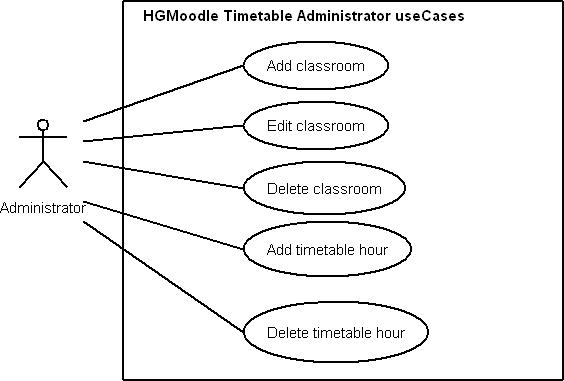
\includegraphics[width=14cm,keepaspectratio]{img/UseCases-Administrator-1r.jpg}
		\caption[List caption]{Casos d'ús per l'administrador.}
		\label{fig:UseCases-Administrator-1r}
		\end{center}
		\end{figure}
Encarregat de gestionar (crear,editar,esborrar) les aules.\\
El fet de gestionar les aules implica tenir-hi assignat per cadascuna d’elles com a mínim un identificador. També seria possible tenir com a atribut la capacitat de l’aula.\\
L'altra parametrització que farà l'administrador serà introduir les hores lectives al llarg del dia i els dies lectius de la setmana.\\
\subsection{Professor}
		\begin{figure}[H] %Here overriding the specifications of Latex good placement
		\begin{center}
		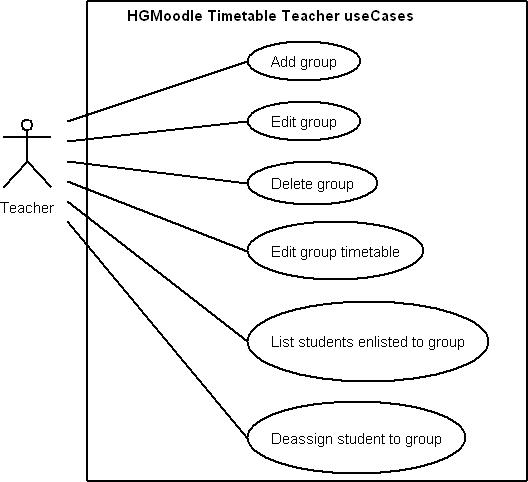
\includegraphics[width=14cm,keepaspectratio]{img/UseCases-Teacher-1r.jpg}
		\caption[List caption]{Casos d'ús per al professor.}
		\label{fig:UseCases-Teacher-1r}
		\end{center}
		\end{figure}
Encarregat de gestionar els grups.\\ 
Els grups tindran com a mínim un identificador, així com també el numero d’alumnes assignats per cada grup. Establir un horari  serà el cas en que el professor li haurà d’assignar un horari i una aula disponibles per la seva classe. Tindrà també l’opció de permetre o no als alumnes canviar-se de grup.\\
Per ultim podra veure el llistat d'alumnes apuntat a cada grup i podrà desassignar-lo si cal.\\
\subsection{Alumne}
		\begin{figure}[H] %Here overriding the specifications of Latex good placement
		\begin{center}
		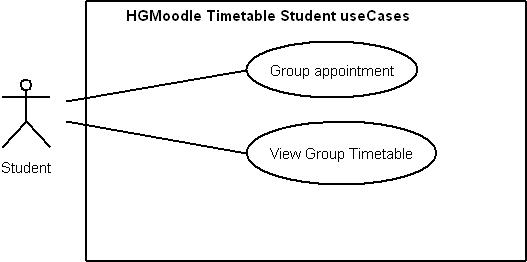
\includegraphics[width=14cm,keepaspectratio]{img/UseCases-Student-1r.jpg}
		\caption[List caption]{Casos d'ús per a l'estudiant.}
		\label{fig:UseCases-Student-1r}
		\end{center}
		\end{figure}
Únicament tenen el cas de apuntar-s'hi a un grup dels creats. Si ja està apuntat tindrà la possibilitat de visualitzar l'horari del grup al qual s'ha assignat i canviar de grup si el professor permet aquesta acció.

\section{Entitat-Relació}

En els següents subapartats es mostra una enumeració de les entitats que intervenen dins el sistema (secció \ref{entitats-1r}, pàgina \pageref{entitats-1r}) i la relació que hi ha entre elles (secció \ref{relacions-1r}, pàgina \pageref{relacions-1r}).
\subsection{Entitats}\label{entitats-1r}

\fbox{
\begin{minipage}{6.4cm}
{\bfseries Grup}\\
Identificador\\
N\'umero d'alumnes\\
\end{minipage}
}
\     \
\hfill
\fbox{
\begin{minipage}{6.4cm}
{\bfseries Timetable}\\
Identificador\\
Identificador Curs\\
\end{minipage}
}
\     \ \\ \     \ \\ \     \ \\
\fbox{
\begin{minipage}{6.4cm}
{\bfseries Hores v\`alides}\\
Hora d'inici\\
Hora de fi\\
\end{minipage}
}
\     \
\hfill
\fbox{
\begin{minipage}{6.4cm}
{\bfseries Horari}\\
Hora inici\\
Hora fi\\
Dia setmanal\\
Identificador de grup\\
Identificador de aula\\
Identificador Curs\\
\end{minipage}
}
\     \ \\ \     \ \\ \     \ \\
\fbox{
\begin{minipage}{6.4cm}
{\bfseries Professor\_Grup}\\
Identificador Professor\\
Identificador Grup\\
\end{minipage}
}
\     \
\hfill
\fbox{
\begin{minipage}{6.4cm}
{\bfseries Aula}\\
Identificador\\
Capacitat\\
\end{minipage}
}
\     \ \\ \     \ \\ \     \ \\
\fbox{
\begin{minipage}{6.4cm}
{\bfseries Alumne\_Grup}\\
Identificador Alumne\\
Identificador Grup\\
\end{minipage}
}
\     \
\hfill
\fbox{
\begin{minipage}{6.4cm}
{\bfseries Dies lectius}\\
Nom del dia setmanal\\
\end{minipage}
}
%\     \ \\ \     \ \\ \     \ \\
\subsection{Relacions}\label{relacions-1r}
		\begin{figure}[H] %Here overriding the specifications of Latex good placement
		\begin{center}
		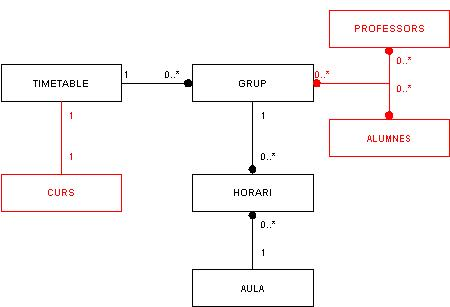
\includegraphics[width=14cm,keepaspectratio]{img/DiagramaRelacions-1r.jpg}
		\caption[List caption]{Diagrama de relacions entre les entitats. En vermell entitats ja existents a Moodle.}
		\label{fig:DiagramaRelacions-1r}
		\end{center}
		\end{figure}
Un grup en un horari, està situat en una aula. A una aula, en un horari determinat només hi haurà com a màxim un grup (o cap). Un grup repetirà a una aula n cops.\\
Cada assignació tindrà una durada, és a dir, tindrà una data d’inici i una data de fi.\\
Es considera que cada grup a una hora determinada i un dia setmanal  determinat estarà situat en una aula (que sempre serà la mateixa). Això vol dir, que durant una setmana en diferents dies de la setmana i en una hora determinada d’aquest dia de la setmana un grup estarà a l’aula que te assignada. És a dir, un professor assignarà una aula, i independentment d’aquesta assignació el grup tindrà un horari setmanal.\\
Professor i Alumne i Curs són entitats que són gestionades pel Moodle, s’haurà de veure de quina manera s’obtenen aquestes dades, però no les gestionarà aquesta aplicació.\\
Cada grup es gestionat per algun o alguns professors (o cap).Cada alumne pertany a un grup (o cap).
\section{Esquema bàsic de la base de dades}
Diagrama extret de la base de dades, per representar explícitament les taules i els camps necessàris i les relacions entre aquestes taules.
		\begin{figure}[H] %Here overriding the specifications of Latex good placement
		\begin{center}
		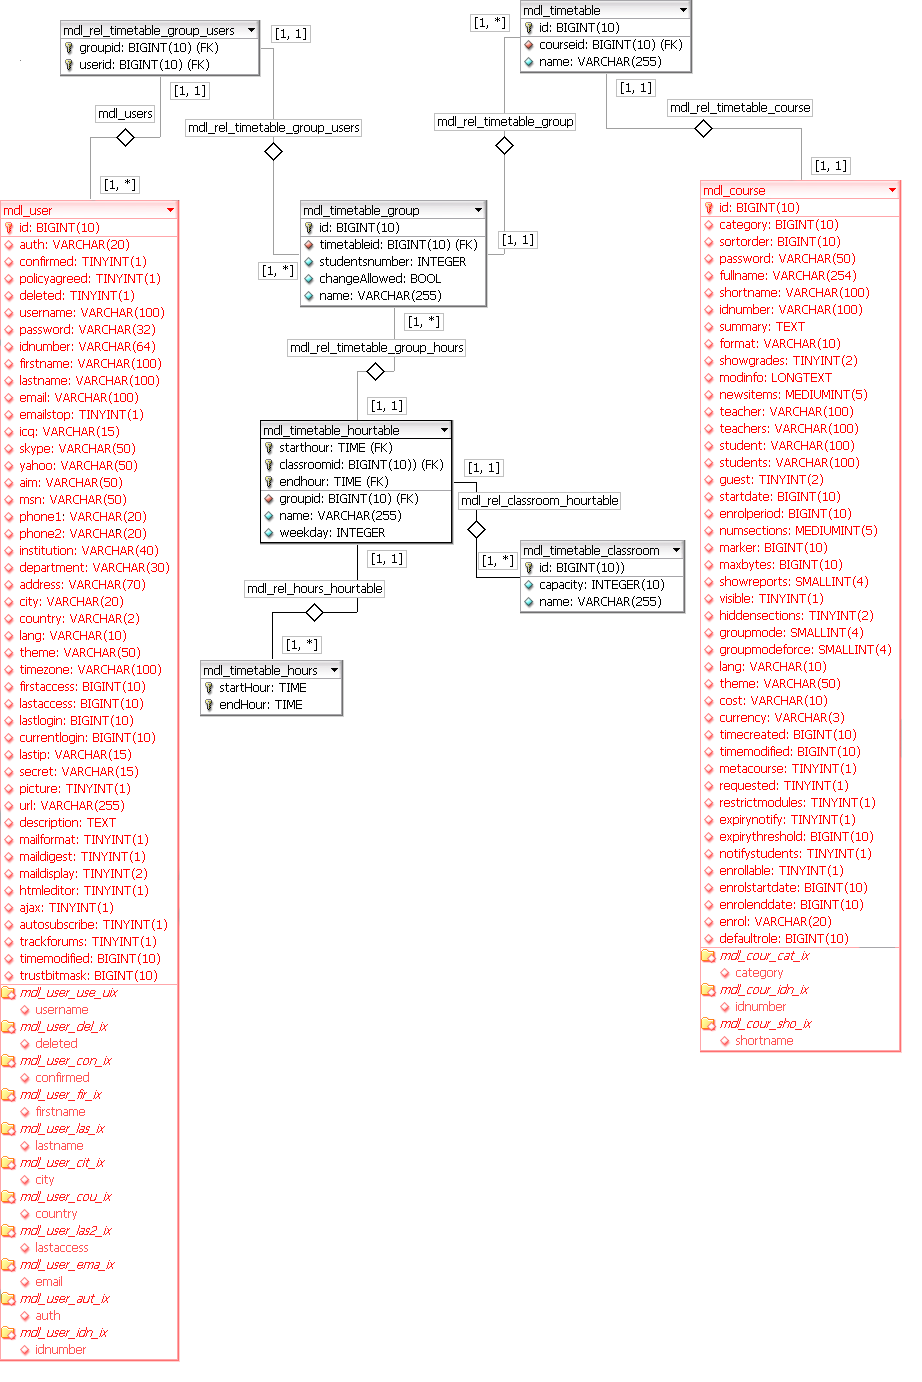
\includegraphics[width=0.90\textwidth,keepaspectratio]{img/DiagramaBBDD-1r.png}
		\caption[List caption]{Esquema de la base de dades. En vermell taules de Moodle.}
		\label{fig:DiagramaBBDD-1r}
		\end{center}
		\end{figure}
\section{Fitxer xmldb per la creació de taules}\label{xmldb-1r}
Tal com s'explica en la secció \ref{AnalisiBasededades} (pàgina \pageref{AnalisiBasededades}) aquest és el fitxer que necessita Moodle per crear les taules necessàries sense haver de creat scripts especialitzats per cadascún dels sistemes gestors de base de dades en els que es vulgui fer compatible el mòdul o bloc.\\
És tracta, doncs, d'un fitxer XML que serveix com capa d'abstracció entre el desenvolupament i la base de dades.
\begin{lstlisting}[style=XML,caption=Fitxer xmldb install.xml per la creació de les taules]
<?xml version="1.0" encoding="UTF-8" ?>
<XMLDB PATH="blocks/timetable/db" VERSION="20070922" COMMENT="XMLDB file for Moodle blocks/timetable"
    xmlns:xsi="http://www.w3.org/2001/XMLSchema-instance"
    xsi:noNamespaceSchemaLocation="../../../lib/xmldb/xmldb.xsd">
  <TABLES>
    <TABLE NAME="timetable_hours" COMMENT="timetable_hours table retrofitted from MySQL" NEXT="timetable_classroom">
      <FIELDS>
        <FIELD NAME="starthour" TYPE="time" LENGTH="small" NOTNULL="true" SEQUENCE="false" ENUM="false" NEXT="endhour"/>
        <FIELD NAME="endhour" TYPE="time" LENGTH="small" NOTNULL="true" SEQUENCE="false" ENUM="false" PREVIOUS="starthour"/>
      </FIELDS>
      <KEYS>
        <KEY NAME="primary" TYPE="primary" FIELDS="starthour, endhour" COMMENT="Primary key for timetable_hours"/>
      </KEYS>
    </TABLE>
    <TABLE NAME="timetable_classroom" COMMENT="timetable_classroom table retrofitted from MySQL" PREVIOUS="timetable_hours" NEXT="timetable">
      <FIELDS>
        <FIELD NAME="id" TYPE="int" LENGTH="10" NOTNULL="true" UNSIGNED="true" SEQUENCE="true" ENUM="false" NEXT="capacity"/>
        <FIELD NAME="capacity" TYPE="int" LENGTH="10" NOTNULL="true" UNSIGNED="true" SEQUENCE="false" ENUM="false" PREVIOUS="id" NEXT="name"/>
        <FIELD NAME="name" TYPE="char" LENGTH="255" NOTNULL="true" SEQUENCE="false" ENUM="false" PREVIOUS="capacity"/>
      </FIELDS>
      <KEYS>
        <KEY NAME="primary" TYPE="primary" FIELDS="id" COMMENT="Primary key for timetable_classroom"/>
      </KEYS>
    </TABLE>
    <TABLE NAME="timetable" COMMENT="timetable table retrofitted from MySQL" PREVIOUS="timetable_classroom" NEXT="timetable_group">
      <FIELDS>
        <FIELD NAME="id" TYPE="int" LENGTH="10" NOTNULL="true" UNSIGNED="true" SEQUENCE="true" ENUM="false" NEXT="courseid"/>
        <FIELD NAME="courseid" TYPE="int" LENGTH="10" NOTNULL="true" UNSIGNED="false" SEQUENCE="false" ENUM="false" PREVIOUS="id" NEXT="name"/>
        <FIELD NAME="name" TYPE="char" LENGTH="255" NOTNULL="false" SEQUENCE="false" ENUM="false" PREVIOUS="courseid"/>
      </FIELDS>
      <KEYS>
        <KEY NAME="primary" TYPE="primary" FIELDS="id" COMMENT="Primary key for timetable" NEXT="timetablecourseid" />
		<KEY NAME="timetablecourseid" TYPE="foreign" FIELDS="courseid" REFTABLE="course" REFFIELDS="id" PREVIOUS="primary" />
      </KEYS>
      <INDEXES>
        <INDEX NAME="courseid" UNIQUE="false" FIELDS="courseid"/>
      </INDEXES>
    </TABLE>
    <TABLE NAME="timetable_group" COMMENT="timetable_group table retrofitted from MySQL" PREVIOUS="timetable" NEXT="timetable_users">
      <FIELDS>
        <FIELD NAME="id" TYPE="int" LENGTH="10" NOTNULL="true" UNSIGNED="true" SEQUENCE="true" ENUM="false" NEXT="timetableid"/>
        <FIELD NAME="timetableid" TYPE="int" LENGTH="10" NOTNULL="true" UNSIGNED="false" SEQUENCE="false" ENUM="false" PREVIOUS="id" NEXT="studentsnumber"/>
        <FIELD NAME="studentsnumber" TYPE="int" LENGTH="10" NOTNULL="false" UNSIGNED="true" SEQUENCE="false" ENUM="false" PREVIOUS="timetableid" NEXT="changeallowed"/>
        <FIELD NAME="changeallowed" TYPE="int" LENGTH="1" NOTNULL="false" UNSIGNED="false" SEQUENCE="false" ENUM="false" PREVIOUS="studentsnumber" NEXT="name"/>
        <FIELD NAME="name" TYPE="char" LENGTH="255" NOTNULL="false" SEQUENCE="false" ENUM="false" PREVIOUS="changeallowed"/>
      </FIELDS>
      <KEYS>
        <KEY NAME="primary" TYPE="primary" FIELDS="id" COMMENT="Primary key for timetable_group" NEXT="grouptimetableid"/>
		<KEY NAME="grouptimetableid" TYPE="foreign" FIELDS="timetableid" REFTABLE="timetable" REFFIELDS="id" PREVIOUS="primary" />
      </KEYS>
      <INDEXES>
        <INDEX NAME="timetableid" UNIQUE="false" FIELDS="timetableid"/>
      </INDEXES>
    </TABLE>
    <TABLE NAME="timetable_users" COMMENT="timetable_users table retrofitted from MySQL" PREVIOUS="timetable_group" NEXT="timetable_hourtable">
      <FIELDS>
        <FIELD NAME="groupid" TYPE="int" LENGTH="10" NOTNULL="true" UNSIGNED="false" SEQUENCE="false" ENUM="false" NEXT="userid"/>
        <FIELD NAME="userid" TYPE="int" LENGTH="10" NOTNULL="true" UNSIGNED="false" SEQUENCE="false" ENUM="false" PREVIOUS="groupid"/>
      </FIELDS>
      <KEYS>
        <KEY NAME="primary" TYPE="primary" FIELDS="groupid, userid" COMMENT="Primary key for timetable_users" NEXT="usergroupid"/>
		<KEY NAME="usergroupid" TYPE="foreign" FIELDS="groupid" REFTABLE="timetable_group" REFFIELDS="id" PREVIOUS="primary" NEXT="useruserid" />
		<KEY NAME="useruserid" TYPE="foreign" FIELDS="userid" REFTABLE="users" REFFIELDS="id" PREVIOUS="usergroupid" />
      </KEYS>
      <INDEXES>
        <INDEX NAME="userid" UNIQUE="false" FIELDS="userid"/>
      </INDEXES>
    </TABLE>
    <TABLE NAME="timetable_hourtable" COMMENT="timetable_hourtable table retrofitted from MySQL" PREVIOUS="timetable_users">
      <FIELDS>
        <FIELD NAME="starthour" TYPE="text" LENGTH="small" NOTNULL="true" SEQUENCE="false" ENUM="false" NEXT="weekday"/>
        <FIELD NAME="weekday" TYPE="char" LENGTH="1" NOTNULL="true" SEQUENCE="false" ENUM="false" PREVIOUS="starthour" NEXT="classroomid"/>
        <FIELD NAME="classroomid" TYPE="int" LENGTH="10" NOTNULL="true" UNSIGNED="false" SEQUENCE="false" ENUM="false" PREVIOUS="weekday" NEXT="endhour"/>
        <FIELD NAME="endhour" TYPE="text" LENGTH="small" NOTNULL="true" SEQUENCE="false" ENUM="false" PREVIOUS="classroomid" NEXT="groupid"/>
        <FIELD NAME="groupid" TYPE="int" LENGTH="10" NOTNULL="true" UNSIGNED="false" SEQUENCE="false" ENUM="false" PREVIOUS="endhour" NEXT="name"/>
        <FIELD NAME="name" TYPE="char" LENGTH="255" NOTNULL="false" SEQUENCE="false" ENUM="false" PREVIOUS="groupid"/>
      </FIELDS>
      <KEYS>
        <KEY NAME="primary" TYPE="primary" FIELDS="starthour, weekday, groupid, classroomid, endhour" COMMENT="Primary key for timetable_hourtable" NEXT="starthourendhour" />
		<KEY NAME="starthourendhour" TYPE="foreign" FIELDS="starthour,endhour" REFTABLE="timetable_hours" REFFIELDS="starthour,endhour" PREVIOUS="primary" NEXT="hourtableclassroomid"/>
		<KEY NAME="hourtableclassroomid" TYPE="foreign" FIELDS="classroomid" REFTABLE="timetable_classroom" REFFIELDS="id" PREVIOUS="starthourendhour" NEXT="hourtablegroupid" />
		<KEY NAME="hourtablegroupid" TYPE="foreign" FIELDS="groupid" REFTABLE="timetable_group" REFFIELDS="id" PREVIOUS="hourtableclassroomid"/>
      </KEYS>
      <INDEXES>
        <INDEX NAME="classroomid" UNIQUE="false" FIELDS="classroomid" NEXT="starthour"/>
        <INDEX NAME="starthour" UNIQUE="false" FIELDS="starthour, endhour" PREVIOUS="classroomid" NEXT="groupid"/>
        <INDEX NAME="groupid" UNIQUE="false" FIELDS="groupid" PREVIOUS="starthour"/>
      </INDEXES>
    </TABLE>
  </TABLES>
</XMLDB>

\end{lstlisting}
\section{Diagrama d'estats}
La manera d'interactuar de l'usuari dependrà del seu rol i segons aquest les operacions que podrà realitzar cada usuari seràn diferents. Per tant podem interpretar el següent diagrama (Figura ~\ref{fig:DiagramaEstats-1r}) com a visió global del funcionament del sistema.
		\begin{figure}[H] %Here overriding the specifications of Latex good placement
		\begin{center}
		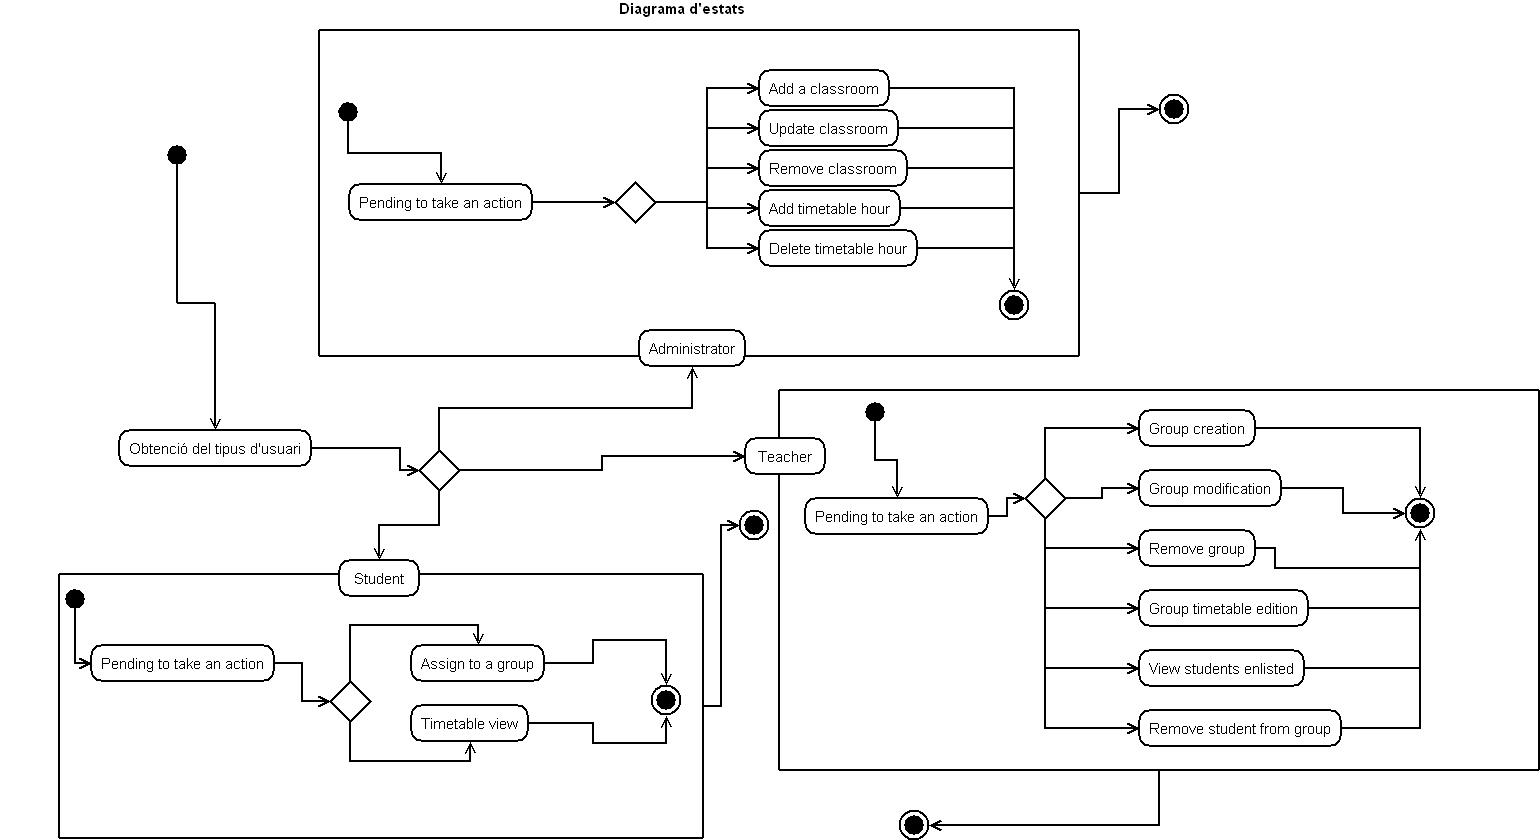
\includegraphics[width=14cm,keepaspectratio]{img/DiagramaEstats-1r.jpg}
		\caption[List caption]{Diagrama de estats del sistema.}
		\label{fig:DiagramaEstats-1r}
		\end{center}
		\end{figure}
\section{Interfície d'usuari}
Les pantalles amb les que els usuaris interaccionaran amb el sistema seran aproximadament així, ja que es tracta d'un primera aproximació al que podria ser la interfície d'usuari
\subsection{Administrador}
Administrador, interfície (Figura ~\ref{fig:Administrator-Timetable}) per gestionar aules, creació, modificació i eliminació. 
		\begin{figure}[H] %Here overriding the specifications of Latex good placement
		\begin{center}
		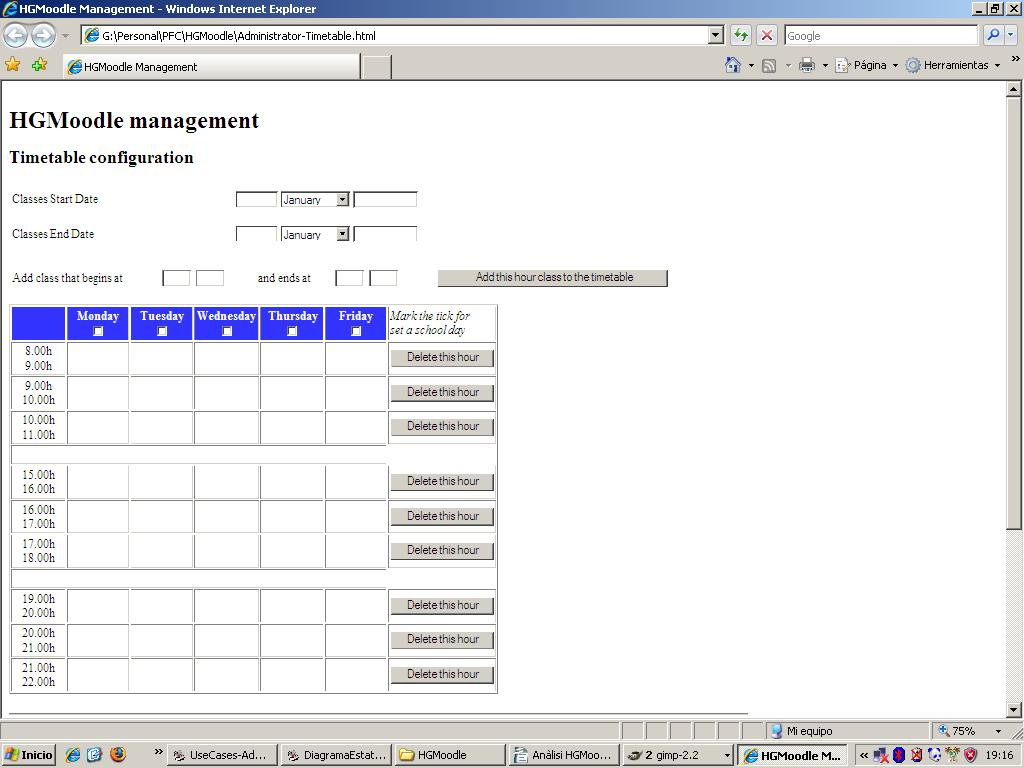
\includegraphics[width=12cm,height=10cm]{img/Administrator-Timetable.jpg}
		\caption[List caption]{Interfície per gestionar aules.}
		\label{fig:Administrator-Timetable}
		\end{center}
		\end{figure}
Interfície (Figura ~\ref{fig:Administrator-Timetable-2}) per manegar les hores lectives i dies lectius del centre i diversos parametres de configuració.
		\begin{figure}[H] %Here overriding the specifications of Latex good placement
		\begin{center}
		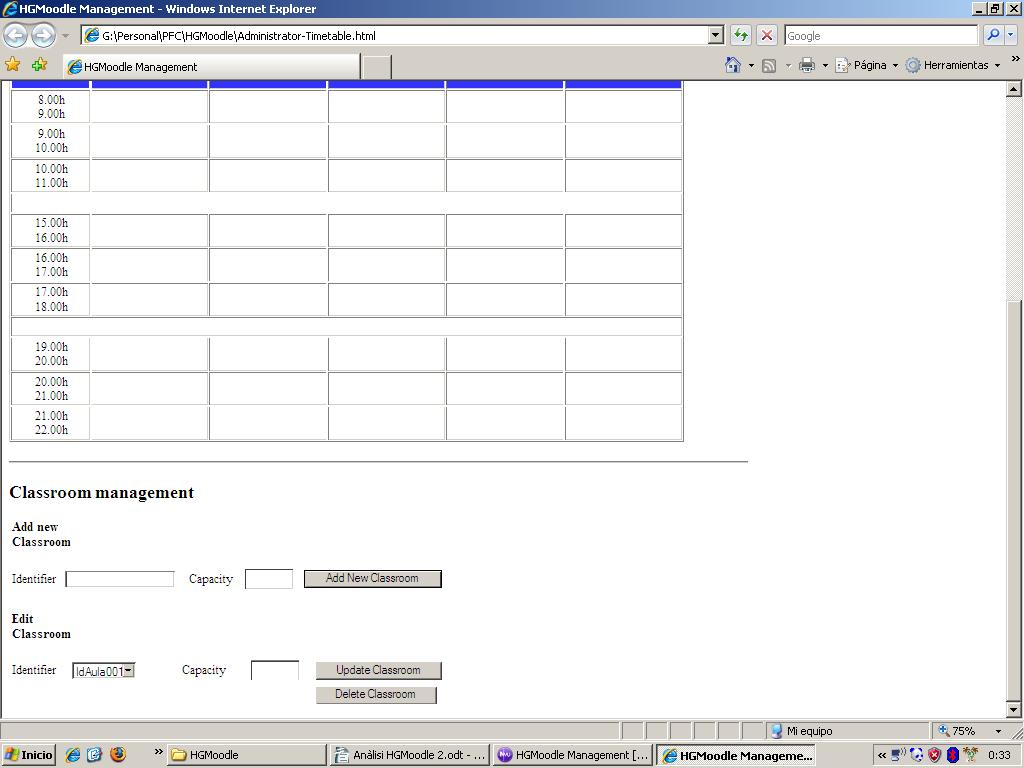
\includegraphics[width=12cm,height=10cm]{img/Administrator-Timetable-2.jpg}
		\caption[List caption]{Interfície per gestionar aules.}
		\label{fig:Administrator-Timetable-2}
		\end{center}
		\end{figure}

\subsection{Professor}
Professor, interfície (Figura ~\ref{fig:Teacher-Timetable}) per assignar horaris i aules a grups i manegar grups. 
		\begin{figure}[H] %Here overriding the specifications of Latex good placement
		\begin{center}
		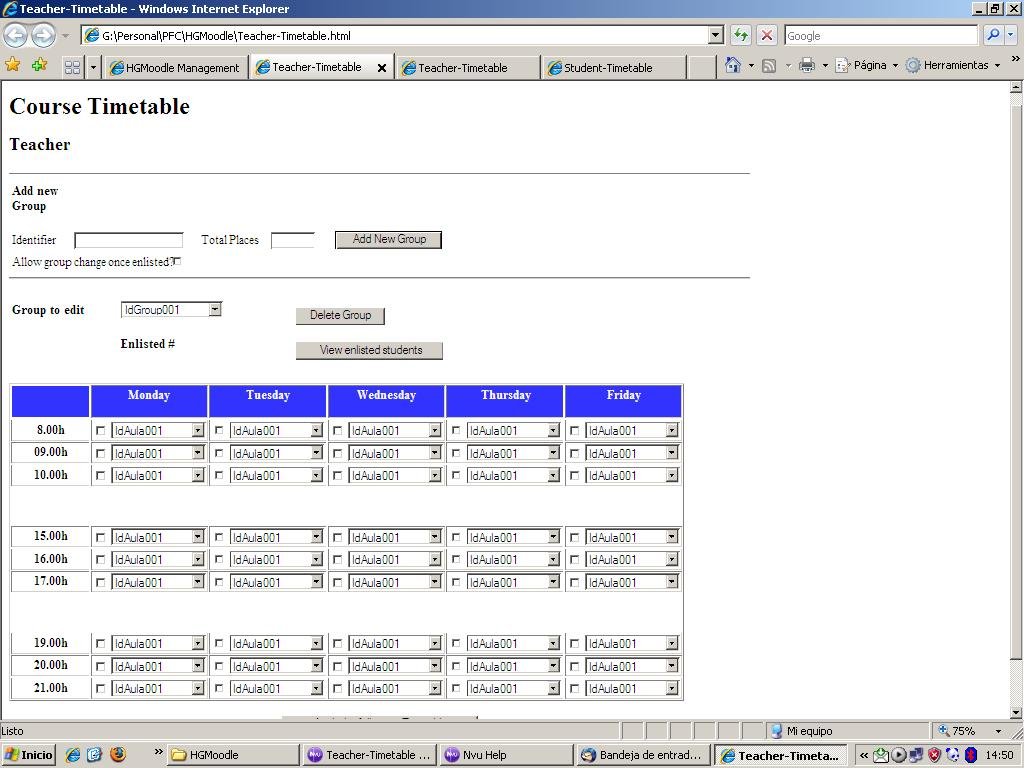
\includegraphics[width=12cm,height=10cm]{img/Teacher-Timetable.jpg}
		\caption[List caption]{Interfície per gestionar horaris de grups.}
		\label{fig:Teacher-Timetable}
		\end{center}
		\end{figure}
Professor, visualització (Figura ~\ref{fig:Teacher-Timetable-2}) dels alumnes apuntats al grup i opció de desassignació.
		\begin{figure}[H] %Here overriding the specifications of Latex good placement
		\begin{center}
		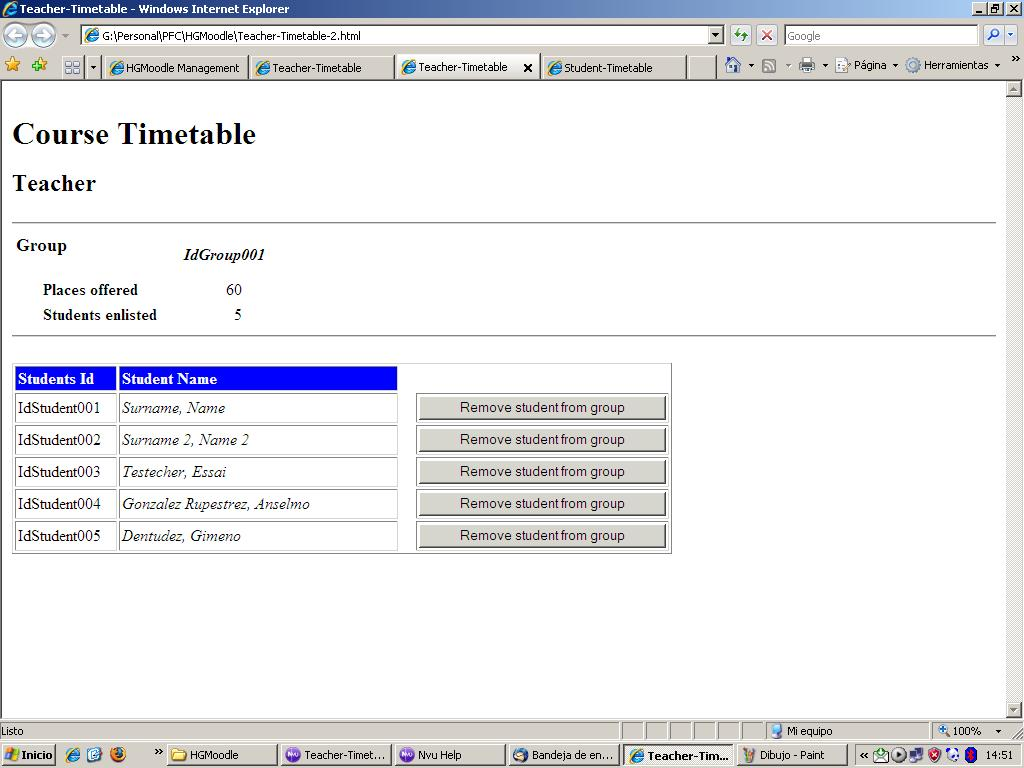
\includegraphics[width=12cm,height=10cm]{img/Teacher-Timetable-2.jpg}
		\caption[List caption]{Visualització llistat d\'alumnes.}
		\label{fig:Teacher-Timetable-2}
		\end{center}
		\end{figure}
\subsection{Alumne}
Alumne, interfície (Figura ~\ref{fig:Student-Timetable}) per apuntar-se als grups.
		\begin{figure}[H] %Here overriding the specifications of Latex good placement
		\begin{center}
		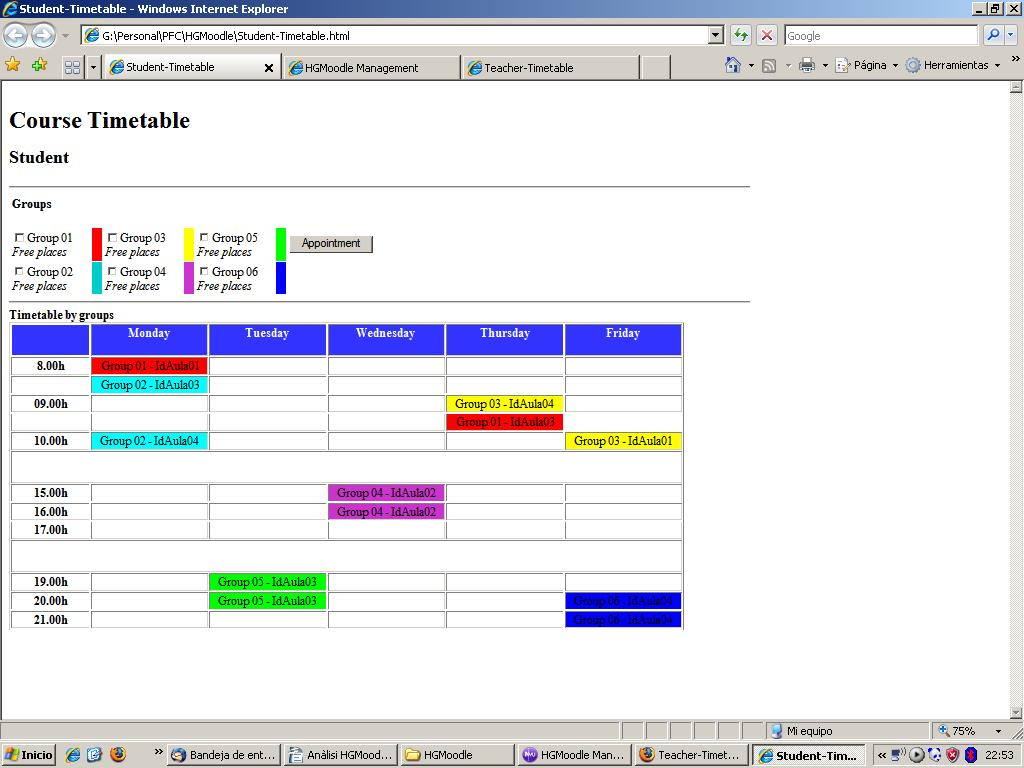
\includegraphics[width=12cm,height=10cm]{img/Student-Timetable.jpg}
		\caption[List caption]{Interfície per apuntar-se a grups.}
		\label{fig:Student-Timetable}
		\end{center}
		\end{figure}
\chapter{Especificació funcional – Revisió final}
Aquest capítol recull la informació necessària a partir de la qual, es podria començar a desenvolupar el mòdul. En aquest cas ja estàn contemplades totes les decissions posteriors al plantejament inicial com ara el control de l'assistència dels alumnes per part dels professors o els canvis en les decissions de disseny que haguessin pogut ser produides degut a problemes durant la fase de desenvolupament.\\
És a dir, en aquest capítol trobem la informació necessària per poder començar el desenvolupament del block en cas que s'hagués de tornar a implementar de nou, tenint en compte els problemes que s'han trobat a l'hora de desenvolupar-lo.
\section{Casos d'ús}
S’adjunta imatge (Figures ~\ref{fig:UseCases-Administrator-rf}, ~\ref{fig:UseCases-Teacher-rf} i ~\ref{fig:UseCases-Student-rf}). Hi hauran tres rols per aquesta aplicació:
\subsection{Administrador}
		\begin{figure}[H] %Here overriding the specifications of Latex good placement
		\begin{center}
		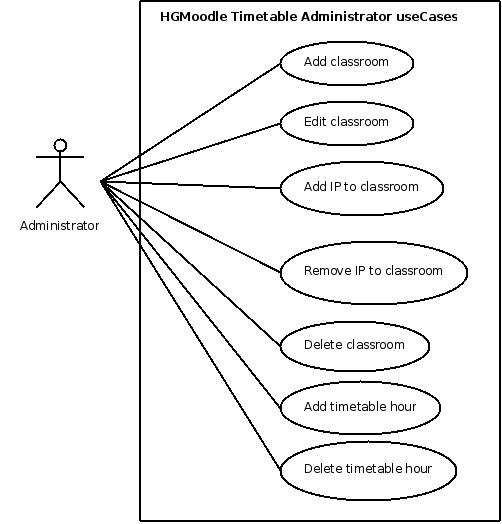
\includegraphics[width=14cm,keepaspectratio]{img/UseCases-Administrator-rf.jpg}
		\caption[List caption]{Casos d'ús per a l'administrador.}
		\label{fig:UseCases-Administrator-rf}
		\end{center}
		\end{figure}
Encarregat de gestionar (crear,editar,esborrar) les aules.\\  
El fet de gestionar les aules implica tenir-hi assignat per cadascuna d’elles com a mínim un identificador. També seria possible tenir com a atribut la capacitat de l’aula.\\
L'altra parametrització que farà l'administrador serà introduir les hores lectives al llarg del dia i els dies lectius de la setmana.\\
Per últim l'administrador es qui gestiona les adreces IP vàlides i s'encarrega d'associar (o des associar) aquestes adreces a cadascuna de les aules físiques.\\
\subsection{Professor}
		\begin{figure}[H] %Here overriding the specifications of Latex good placement
		\begin{center}
		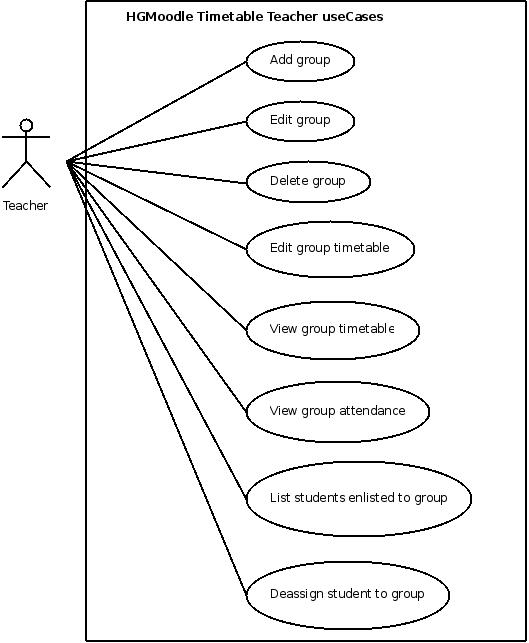
\includegraphics[width=14cm,keepaspectratio]{img/UseCases-Teacher-rf.jpg}
		\caption[List caption]{Casos d'ús per al professor.}
		\label{fig:UseCases-Teacher-rf}
		\end{center}
		\end{figure}
Encarregat de gestionar els grups. \\
Els grups tindran com a mínim un identificador, així com també el numero d’alumnes assignats per cada grup. Establir un horari  serà el cas en que el professor li haurà d’assignar un horari i una aula disponibles per la seva classe. Tindrà també l’opció de permetre o no als alumnes canviar-se de grup.\\
També podrà veure el llistat d'alumnes apuntat a cada grup i podrà des assignar-lo si cal.\\
Per últim els professors tenen la possibilitat d'observar els accessos al sistema Moodle en cada moment que hi ha hagut cadascúna de les classes i comprovar si ha estat un accès des d'una adreça vàlida, de les associades a l'aula per l'administrador. Això li permetrà confirmar l'assistència dels alumnes a les classes.\\
\subsection{Alumne}
		\begin{figure}[H] %Here overriding the specifications of Latex good placement
		\begin{center}
		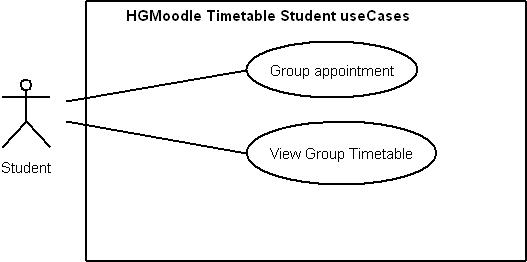
\includegraphics[width=14cm,keepaspectratio]{img/UseCases-Student-rf.jpg}
		\caption[List caption]{Casos d'ús per a l'estudiant.}
		\label{fig:UseCases-Student-rf}
		\end{center}
		\end{figure}
Únicament tenen el cas de apuntar-s’hi a un grup dels creats. Si ja està apuntat tindrà la possibilitat de visualitzar l'horari del grup al qual s'ha assignat i canviar de grup si el professor permet aquesta acció.\\
\section{Entitat-Relació}
En els següents subapartats es mostra una enumeració de les entitats que intervenen dins el sistema (secció \ref{entitats-rf}, pàgina \pageref{entitats-rf}) i la relació que hi ha entre elles (secció \ref{relacions-rf}, pàgina \pageref{relacions-rf}).
\subsection{Entitats}\label{entitats-rf}
A continuació hi ha una representació de la idea de les entitats que s'hauràn de gestionar amb el sistema.\\\	\\
\fbox{
\begin{minipage}{6.4cm}
{\bfseries Grup}\\
Identificador\\
N\'umero d'alumnes\\
\end{minipage}
}
\     \
\hfill
\fbox{
\begin{minipage}{6.4cm}
{\bfseries Timetable}\\
Identificador\\
Identificador Curs\\
\end{minipage}
}
\     \ \\ \     \ \\ \     \ \\
\fbox{
\begin{minipage}{6.4cm}
{\bfseries Hores v\`alides}\\
Hora d'inici\\
Hora de fi\\
\end{minipage}
}
\     \
\hfill
\fbox{
\begin{minipage}{6.4cm}
{\bfseries Horari}\\
Hora inici\\
Hora fi\\
Dia setmanal\\
Identificador de grup\\
Identificador de aula\\
Identificador Curs\\
\end{minipage}
}
\     \ \\ \     \ \\ \     \ \\
\fbox{
\begin{minipage}{6.4cm}
{\bfseries Professor\_Grup}\\
Identificador Professor\\
Identificador Grup\\
\end{minipage}
}
\     \
\hfill
\fbox{
\begin{minipage}{6.4cm}
{\bfseries Aula}\\
Identificador\\
Capacitat\\
\end{minipage}
}
\     \ \\ \     \ \\ \     \ \\
\fbox{
\begin{minipage}{6.4cm}
{\bfseries Alumne\_Grup}\\
Identificador Alumne\\
Identificador Grup\\
\end{minipage}
}
\     \
\hfill
\fbox{
\begin{minipage}{6.4cm}
{\bfseries Dies lectius}\\
Nom del dia setmanal\\
\end{minipage}
}
\     \ \\ \     \ \\ \     \ \\
\fbox{
\begin{minipage}{6.4cm}
{\bfseries Adreça\_IP}\\
Adreça IP\\
Identificador Aula\\
\end{minipage}
}
\     \
\hfill
\fbox{
\begin{minipage}{6.4cm}
{\bfseries Històric de Horari}\\
Data
Hora inici\\
Hora fi\\
Dia setmanal\\
Identificador de grup\\
Identificador de aula\\
Identificador Curs\\
Llista Adreces IP vàlides per data i aula de la classe\\
\end{minipage}
}
\subsection{Relacions}\label{relacions-rf}
		\begin{figure}[H] %Here overriding the specifications of Latex good placement
		\begin{center}
		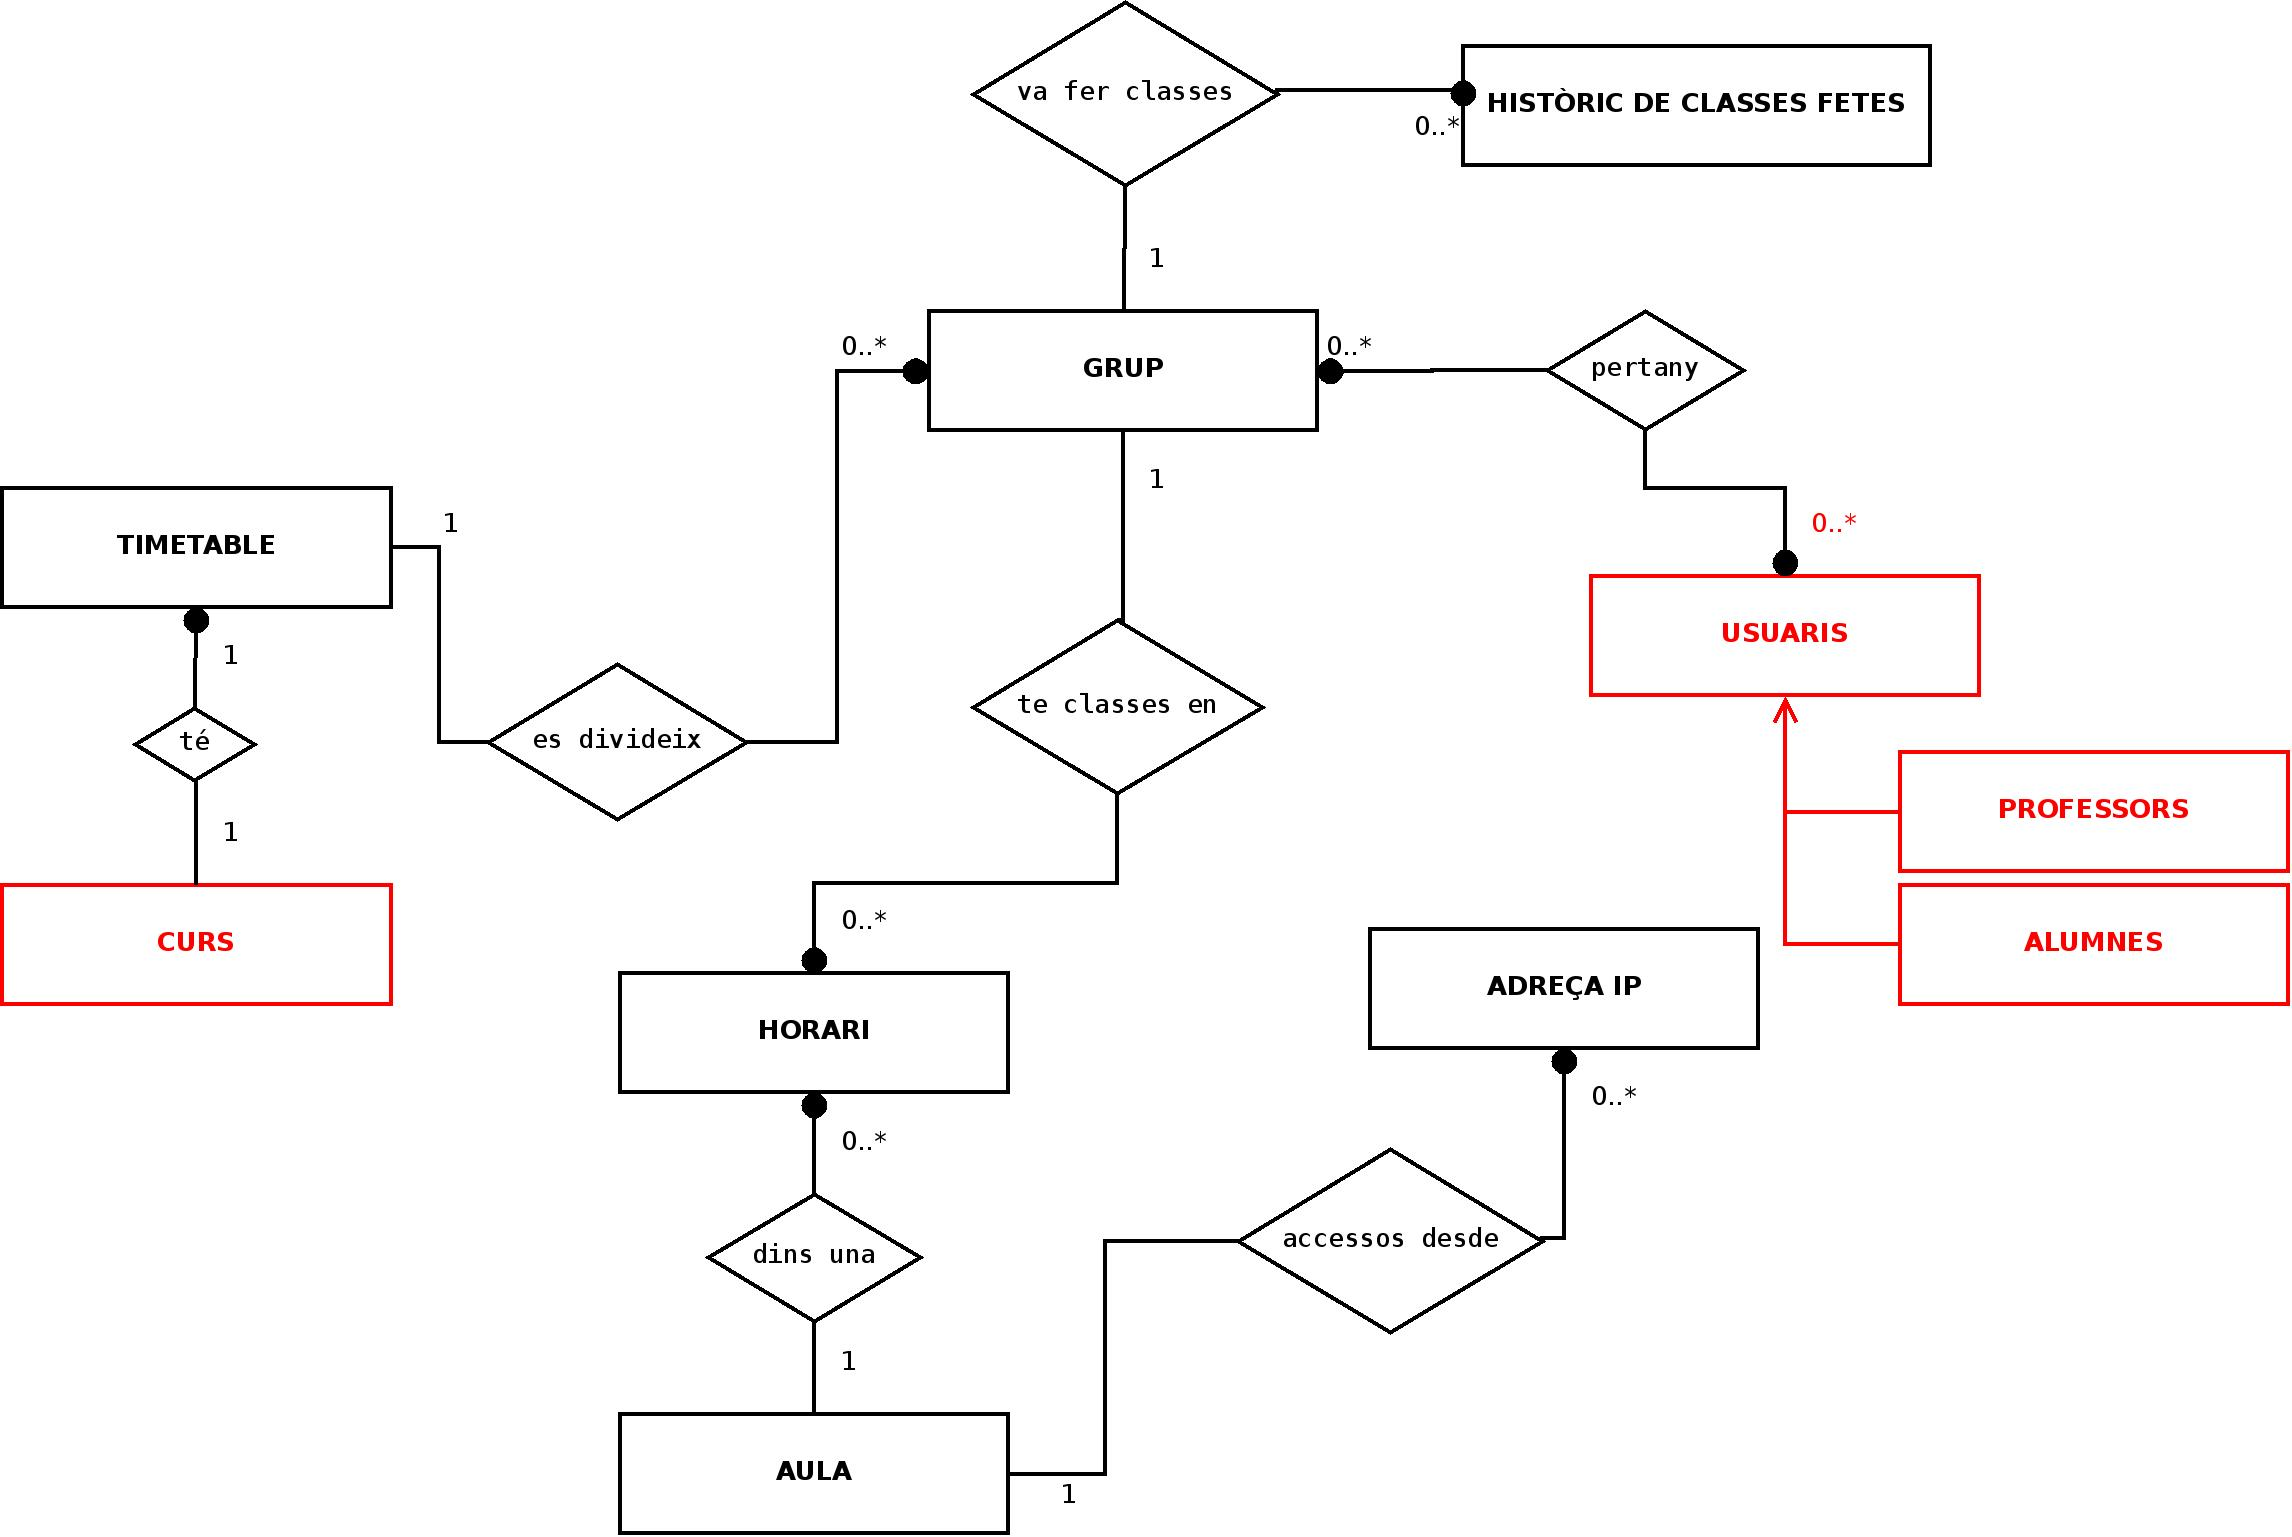
\includegraphics[width=14cm,keepaspectratio]{img/DiagramaRelacions-rf.jpg}
		\caption[List caption]{Diagrama de relacions entre les entitats. En vermell entitats ja existents a Moodle.}
		\label{fig:DiagramaRelacions-rf}
		\end{center}
		\end{figure}
Un grup en un horari, està situat en una aula. A una aula, en un horari determinat només hi haurà com a màxim un grup (o cap). Un grup repetirà a una aula n cops.\\
Cada assignació tindrà una durada, és a dir, tindrà una data d’inici i una data de fi.\\
Es considera que cada grup a una hora determinada i un dia setmanal  determinat estarà situat en una aula (que sempre serà la mateixa). Això vol dir, que durant una setmana en diferents dies de la setmana i en una hora determinada d’aquest dia de la setmana un grup estarà a l’aula que te assignada. És a dir, un professor assignarà una aula, i independentment d’aquesta assignació el grup tindrà un horari setmanal.\\
Totes les classes realitzades per cada grup s'aniran enregistrant a un històric de classes per grup per poder creuar  aquestes dades amb les dades dels accessos pròpies ja del sistema Moodle.\\
Cada aula té unes adreces IP considerades vàlides, cada aula pot tenir assignades varies adreces IP (o cap), una adreça IP pot ser assignada a moltes aules (o cap).\\
Professor i Alumne i Curs són entitats que són gestionades pel Moodle, s’haurà de veure de quina manera s’obtenen aquestes dades, però no les gestionarà aquesta aplicació.\\
Cada grup es gestionat per algun o alguns professors (o cap).Cada alumne pertany a un grup (o cap).\\
\section{Esquema bàsic de la base de dades}
Diagrama extret de la base de dades, per representar explícitament les taules i els camps necessàris i les relacions entre aquestes taules.
		\begin{figure}[H] %Here overriding the specifications of Latex good placement
		\begin{center}
		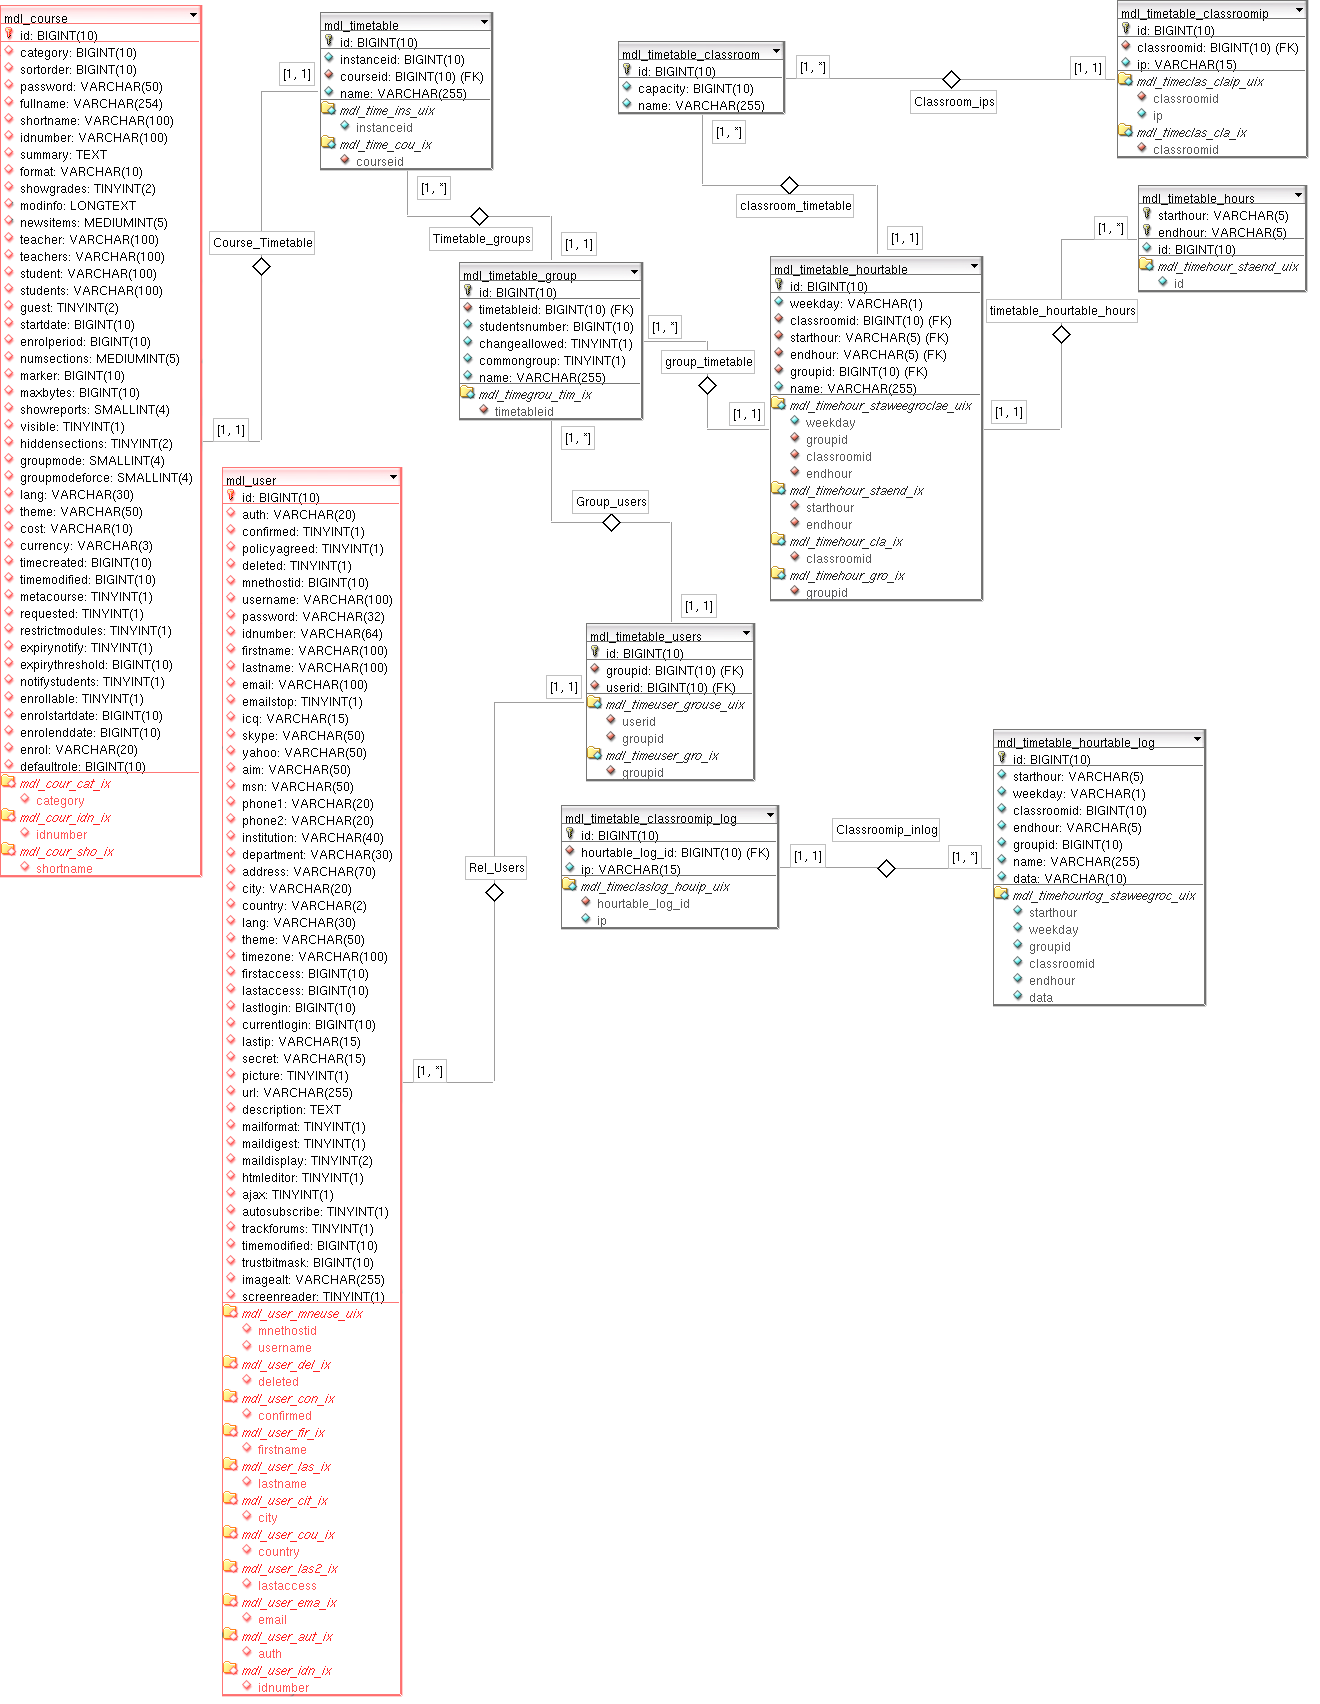
\includegraphics[width=0.90\textwidth,keepaspectratio]{img/DiagramaBBDD-rf.png}
		\caption[List caption]{Esquema de la base de dades. En vermell taules de Moodle.}
		\label{fig:DiagramaBBDD-rf}
		\end{center}
		\end{figure}
\section{Fitxer xmldb per la creació de taules}\label{xmldb-rf}
Tal com s'explica en la secció \ref{AnalisiBasededades} (pàgina \pageref{AnalisiBasededades}) aquest és el fitxer que necessita Moodle per crear les taules necessàries sense haver de creat scripts especialitzats per cadascún dels sistemes gestors de base de dades en els que es vulgui fer compatible el mòdul o bloc.\\
És tracta, doncs, d'un fitxer XML que serveix com capa d'abstracció entre el desenvolupament i la base de dades.
\begin{lstlisting}[style=XML, caption=Fitxer xmldb install.xml per la creació de les taules]
<?xml version="1.0" encoding="UTF-8" ?> 
<XMLDB PATH="blocks/timetable/db" VERSION="20080423" COMMENT="XMLDB file for Moodle blocks/timetable" 
    xmlns:xsi="http://www.w3.org/2001/XMLSchema-instance" 
    xsi:noNamespaceSchemaLocation="../../../lib/xmldb/xmldb.xsd" 
> 
  <TABLES> 
    <TABLE NAME="timetable_hours" COMMENT="timetable_hours table retrofitted from MySQL" NEXT="timetable_classroom"> 
      <FIELDS> 
        <FIELD NAME="id" TYPE="int" LENGTH="10" NOTNULL="true" UNSIGNED="true" SEQUENCE="true" ENUM="false" NEXT="starthour"/> 
		<FIELD NAME="starthour" TYPE="char" LENGTH="5" NOTNULL="true" SEQUENCE="false" ENUM="false" NEXT="endhour" PREVIOUS="id" /> 
        <FIELD NAME="endhour" TYPE="char" LENGTH="5" NOTNULL="true" SEQUENCE="false" ENUM="false" PREVIOUS="starthour"/> 
      </FIELDS> 
      <KEYS> 
		<KEY NAME="primary" TYPE="primary" FIELDS="id" COMMENT="Key for id for timetable_hours" NEXT="starthourendhour"/>  
        <KEY NAME="starthourendhour" TYPE="unique" FIELDS="starthour, endhour" COMMENT="Primary key for timetable_hours" PREVIOUS="primary" /> 
      </KEYS> 
    </TABLE> 
    <TABLE NAME="timetable_classroom" COMMENT="timetable_classroom table retrofitted from MySQL" PREVIOUS="timetable_hours" NEXT="timetable"> 
      <FIELDS> 
        <FIELD NAME="id" TYPE="int" LENGTH="10" NOTNULL="true" UNSIGNED="true" SEQUENCE="true" ENUM="false" NEXT="capacity"/> 
        <FIELD NAME="capacity" TYPE="int" LENGTH="10" NOTNULL="true" UNSIGNED="true" SEQUENCE="false" ENUM="false" PREVIOUS="id" NEXT="name"/> 
        <FIELD NAME="name" TYPE="char" LENGTH="255" NOTNULL="true" SEQUENCE="false" ENUM="false" PREVIOUS="capacity"/> 
      </FIELDS> 
      <KEYS> 
        <KEY NAME="primary" TYPE="primary" FIELDS="id" COMMENT="Primary key for timetable_classroom"  /> 
      </KEYS> 
    </TABLE> 
    <TABLE NAME="timetable" COMMENT="timetable table retrofitted from MySQL" PREVIOUS="timetable_classroom" NEXT="timetable_group"> 
      <FIELDS> 
        <FIELD NAME="id" TYPE="int" LENGTH="10" NOTNULL="true" UNSIGNED="true" ENUM="false" SEQUENCE="true" NEXT="instanceid"/> 
		<FIELD NAME="instanceid" TYPE="int" LENGTH="10" NOTNULL="true" UNSIGNED="true" ENUM="false" SEQUENCE="false" PREVIOUS="id" NEXT="courseid"/> 
        <FIELD NAME="courseid" TYPE="int" LENGTH="10" NOTNULL="true" UNSIGNED="false" SEQUENCE="false" ENUM="false" PREVIOUS="instanceid" NEXT="name"/> 
        <FIELD NAME="name" TYPE="char" LENGTH="255" NOTNULL="false" SEQUENCE="false" ENUM="false" PREVIOUS="courseid"/> 
      </FIELDS> 
      <KEYS> 
	    <KEY NAME="primary" TYPE="primary" FIELDS="id" COMMENT="Primary key for timetable" NEXT="timetablecourseid" /> 
		<KEY NAME="timetablecourseid" TYPE="foreign" FIELDS="courseid" REFTABLE="course" REFFIELDS="id" PREVIOUS="primary" NEXT="instanceid" /> 
		<KEY NAME="instanceid" TYPE="unique" FIELDS="instanceid" COMMENT="Instance key for timetable"  PREVIOUS="timetablecourseid"/> 
      </KEYS> 
      <!--INDEXES> 
        <INDEX NAME="courseid" UNIQUE="false" FIELDS="courseid"/> 
      </INDEXES--> 
    </TABLE> 
    <TABLE NAME="timetable_group" COMMENT="timetable_group table retrofitted from MySQL" PREVIOUS="timetable" NEXT="timetable_users"> 
      <FIELDS> 
        <FIELD NAME="id" TYPE="int" LENGTH="10" NOTNULL="true" UNSIGNED="true" SEQUENCE="true" ENUM="false" NEXT="timetableid"/> 
        <FIELD NAME="timetableid" TYPE="int" LENGTH="10" NOTNULL="true" UNSIGNED="false" SEQUENCE="false" ENUM="false" PREVIOUS="id" NEXT="studentsnumber"/> 
        <FIELD NAME="studentsnumber" TYPE="int" LENGTH="10" NOTNULL="false" UNSIGNED="true" SEQUENCE="false" ENUM="false" PREVIOUS="timetableid" NEXT="changeallowed"/> 
        <FIELD NAME="changeallowed" TYPE="int" LENGTH="1" NOTNULL="false" UNSIGNED="false" SEQUENCE="false" ENUM="false" PREVIOUS="studentsnumber" NEXT="commongroup"/> 
        <FIELD NAME="commongroup" TYPE="int" LENGTH="1" NOTNULL="false" UNSIGNED="false" SEQUENCE="false" ENUM="false" PREVIOUS="changeallowed" NEXT="name"/> 
        <FIELD NAME="name" TYPE="char" LENGTH="255" NOTNULL="false" SEQUENCE="false" ENUM="false" PREVIOUS="commongroup"/> 
      </FIELDS> 
      <KEYS> 
        <KEY NAME="primary" TYPE="primary" FIELDS="id" COMMENT="Primary key for timetable_group" NEXT="grouptimetableid"/> 
		<KEY NAME="grouptimetableid" TYPE="foreign" FIELDS="timetableid" REFTABLE="timetable" REFFIELDS="id" PREVIOUS="primary" /> 
      </KEYS> 
      <!--INDEXES> 
        <INDEX NAME="timetableid" UNIQUE="false" FIELDS="timetableid"/> 
      </INDEXES--> 
    </TABLE> 
    <TABLE NAME="timetable_users" COMMENT="timetable_users table retrofitted from MySQL" PREVIOUS="timetable_group" NEXT="timetable_hourtable"> 
      <FIELDS> 
	    <FIELD NAME="id" TYPE="int" LENGTH="10" NOTNULL="true" UNSIGNED="true" SEQUENCE="true" ENUM="false" NEXT="groupid"/>  
        <FIELD NAME="groupid" TYPE="int" LENGTH="10" NOTNULL="true" UNSIGNED="false" SEQUENCE="false" ENUM="false" NEXT="userid" PREVIOUS="id"/> 
        <FIELD NAME="userid" TYPE="int" LENGTH="10" NOTNULL="true" UNSIGNED="false" SEQUENCE="false" ENUM="false" PREVIOUS="groupid"/> 
      </FIELDS> 
      <KEYS> 
		<KEY NAME="primary" TYPE="primary" FIELDS="id" COMMENT="Key for id for timetable_hours" NEXT="groupiduserid"/>    
        <KEY NAME="groupiduserid" TYPE="unique" FIELDS="groupid, userid" COMMENT="Primary key for timetable_users" NEXT="usergroupid" PREVIOUS="primary"/> 
		<KEY NAME="usergroupid" TYPE="foreign" FIELDS="groupid" REFTABLE="timetable_group" REFFIELDS="id" PREVIOUS="groupiduserid" NEXT="useruserid" /> 
		<KEY NAME="useruserid" TYPE="foreign" FIELDS="userid" REFTABLE="users" REFFIELDS="id" PREVIOUS="usergroupid" /> 
      </KEYS> 
      <!--INDEXES> 
        <INDEX NAME="userid" UNIQUE="false" FIELDS="userid"/> 
      </INDEXES--> 
    </TABLE> 
    <TABLE NAME="timetable_hourtable" COMMENT="timetable_hourtable table retrofitted from MySQL" PREVIOUS="timetable_users" NEXT="timetable_classroomip"> 
      <FIELDS> 
         <FIELD NAME="id" TYPE="int" LENGTH="10" NOTNULL="true" UNSIGNED="true" SEQUENCE="true" ENUM="false" NEXT="starthour"/> 
		<FIELD NAME="starthour" TYPE="char" LENGTH="5" NOTNULL="true" SEQUENCE="false" ENUM="false" NEXT="weekday" PREVIOUS="id" /> 
        <FIELD NAME="weekday" TYPE="char" LENGTH="1" NOTNULL="true" SEQUENCE="false" ENUM="false" PREVIOUS="starthour" NEXT="classroomid"/> 
        <FIELD NAME="classroomid" TYPE="int" LENGTH="10" NOTNULL="true" UNSIGNED="false" SEQUENCE="false" ENUM="false" PREVIOUS="weekday" NEXT="endhour"/> 
        <FIELD NAME="endhour" TYPE="char" LENGTH="5" NOTNULL="true" SEQUENCE="false" ENUM="false" PREVIOUS="classroomid" NEXT="groupid"/> 
        <FIELD NAME="groupid" TYPE="int" LENGTH="10" NOTNULL="true" UNSIGNED="false" SEQUENCE="false" ENUM="false" PREVIOUS="endhour" NEXT="name"/> 
        <FIELD NAME="name" TYPE="char" LENGTH="255" NOTNULL="false" SEQUENCE="false" ENUM="false" PREVIOUS="groupid"/> 
      </FIELDS> 
      <KEYS> 
		<KEY NAME="primary" TYPE="primary" FIELDS="id" COMMENT="Key for id for timetable_hours" NEXT="swgce"/>    
        <KEY NAME="swgce" TYPE="unique" FIELDS="starthour, weekday, groupid, classroomid, endhour" COMMENT="Primary key for timetable_hourtable" NEXT="starthourendhour" PREVIOUS="primary"/> 
		<KEY NAME="starthourendhour" TYPE="foreign" FIELDS="starthour,endhour" REFTABLE="timetable_hours" REFFIELDS="starthour,endhour" PREVIOUS="swgce" NEXT="hourtableclassroomid"/> 
		<KEY NAME="hourtableclassroomid" TYPE="foreign" FIELDS="classroomid" REFTABLE="timetable_classroom" REFFIELDS="id" PREVIOUS="starthourendhour" NEXT="hourtablegroupid" /> 
		<KEY NAME="hourtablegroupid" TYPE="foreign" FIELDS="groupid" REFTABLE="timetable_group" REFFIELDS="id" PREVIOUS="hourtableclassroomid"/> 
      </KEYS> 
      <!--INDEXES> 
        <INDEX NAME="classroomid" UNIQUE="false" FIELDS="classroomid" NEXT="starthour"/> 
        <INDEX NAME="starthour" UNIQUE="false" FIELDS="starthour, endhour" PREVIOUS="classroomid" NEXT="groupid"/> 
        <INDEX NAME="groupid" UNIQUE="false" FIELDS="groupid" PREVIOUS="starthour"/> 
      </INDEXES--> 
    </TABLE> 
	<TABLE NAME="timetable_classroomip" COMMENT="timetable_classroomip" PREVIOUS="timetable_hourtable" NEXT="timetable_hourtable_log" > 
		<FIELDS> 
		    <FIELD NAME="id" TYPE="int" LENGTH="10" NOTNULL="true" UNSIGNED="true" SEQUENCE="true" ENUM="false" NEXT="classroomid"/> 
			<FIELD NAME="classroomid" TYPE="int" LENGTH="10" NOTNULL="true" UNSIGNED="true" SEQUENCE="false" ENUM="false" NEXT="ip" PREVIOUS="id"/> 
			<FIELD NAME="ip" TYPE="char" LENGTH="15" NOTNULL="true" UNSIGNED="true" SEQUENCE="false" ENUM="false" PREVIOUS="classroomid"/> 
		</FIELDS> 
		<KEYS> 
			<KEY NAME="primary" TYPE="primary" FIELDS="id" COMMENT="Key for id for timetable_hours" NEXT="classroomidip"/>  
			<KEY NAME="classroomidip" TYPE="unique" FIELDS="classroomid,ip" NEXT="classroomipclassroom" PREVIOUS="primary"/> 
			<KEY NAME="classroomipclassroom" TYPE="foreign" FIELDS="classroomid" REFTABLE="timetable_classroom" REFFIELDS="id" PREVIOUS="classroomidip" /> 
		</KEYS> 
	</TABLE> 
	<TABLE NAME="timetable_hourtable_log" COMMENT="timetable_hourtable_log" PREVIOUS="timetable_classroomip" NEXT="timetable_classroomip_log" > 
		<FIELDS> 
			<FIELD NAME="id" TYPE="int" LENGTH="10" NOTNULL="true" UNSIGNED="true" SEQUENCE="true" ENUM="false" NEXT="starthour"/> 
			<FIELD NAME="starthour" TYPE="char" LENGTH="5" NOTNULL="true" SEQUENCE="false" ENUM="false" NEXT="weekday" PREVIOUS="id" /> 
        <FIELD NAME="weekday" TYPE="char" LENGTH="1" NOTNULL="true" SEQUENCE="false" ENUM="false" PREVIOUS="starthour" NEXT="classroomid"/> 
        <FIELD NAME="classroomid" TYPE="int" LENGTH="10" NOTNULL="true" UNSIGNED="false" SEQUENCE="false" ENUM="false" PREVIOUS="weekday" NEXT="endhour"/> 
        <FIELD NAME="endhour" TYPE="char" LENGTH="5" NOTNULL="true" SEQUENCE="false" ENUM="false" PREVIOUS="classroomid" NEXT="groupid"/> 
        <FIELD NAME="groupid" TYPE="int" LENGTH="10" NOTNULL="true" UNSIGNED="false" SEQUENCE="false" ENUM="false" PREVIOUS="endhour" NEXT="name"/> 
        <FIELD NAME="name" TYPE="char" LENGTH="255" NOTNULL="false" SEQUENCE="false" ENUM="false" PREVIOUS="groupid" NEXT="data"/> 
		<FIELD NAME="data" TYPE="char" LENGTH="10" NOTNULL="true" SEQUENCE="false" ENUM="false" PREVIOUS="name" /> 
      </FIELDS> 
		    <KEYS> 
				<KEY NAME="primary" TYPE="primary" FIELDS="id" COMMENT="Key for id for timetable_hours" NEXT="swgced"/>   
				<KEY NAME="swgced" TYPE="unique" FIELDS="starthour, weekday, groupid, classroomid, endhour,data" COMMENT="Primary key for timetable_hourtable"  PREVIOUS="primary"/> 
			</KEYS> 
	</TABLE> 
	<TABLE NAME="timetable_classroomip_log" COMMENT="timetable_classroomip_log" PREVIOUS="timetable_hourtable_log"> 
		<FIELDS> 
			<FIELD NAME="id" TYPE="int" LENGTH="10" NOTNULL="true" UNSIGNED="true" SEQUENCE="true" ENUM="false" NEXT="hourtable_log_id"/> 
			<FIELD NAME="hourtable_log_id" TYPE="int" LENGTH="10" NOTNULL="true" UNSIGNED="false" SEQUENCE="false" ENUM="false" PREVIOUS="id" NEXT="ip"/> 
			<FIELD NAME="ip" TYPE="char" LENGTH="15" NOTNULL="true" UNSIGNED="true" SEQUENCE="false" ENUM="false" PREVIOUS="hourtable_log_id"/> 
		</FIELDS> 
		<KEYS> 
				<KEY NAME="primary" TYPE="primary" FIELDS="id" COMMENT="Key for id for timetable_hours" NEXT="hliip"/>   
				<KEY NAME="hliip" TYPE="unique" FIELDS="hourtable_log_id,ip" COMMENT="Primary key for timetable_classroom"  PREVIOUS="primary"/> 
		</KEYS> 
	</TABLE> 
  </TABLES> 
</XMLDB>
\end{lstlisting}
\section{Diagrama d'estats}
La manera d'interaccionar de l'usuari dependrà del seu rol i segons aquest les operacions que podrà realitzar cada usuari seran diferents. Per tant podem interpretar el següent diagrama (Figura ~\ref{fig:DiagramaEstats-rf}) com a visió global del funcionament del sistema.
		\begin{figure}[H] %Here overriding the specifications of Latex good placement
		\begin{center}
		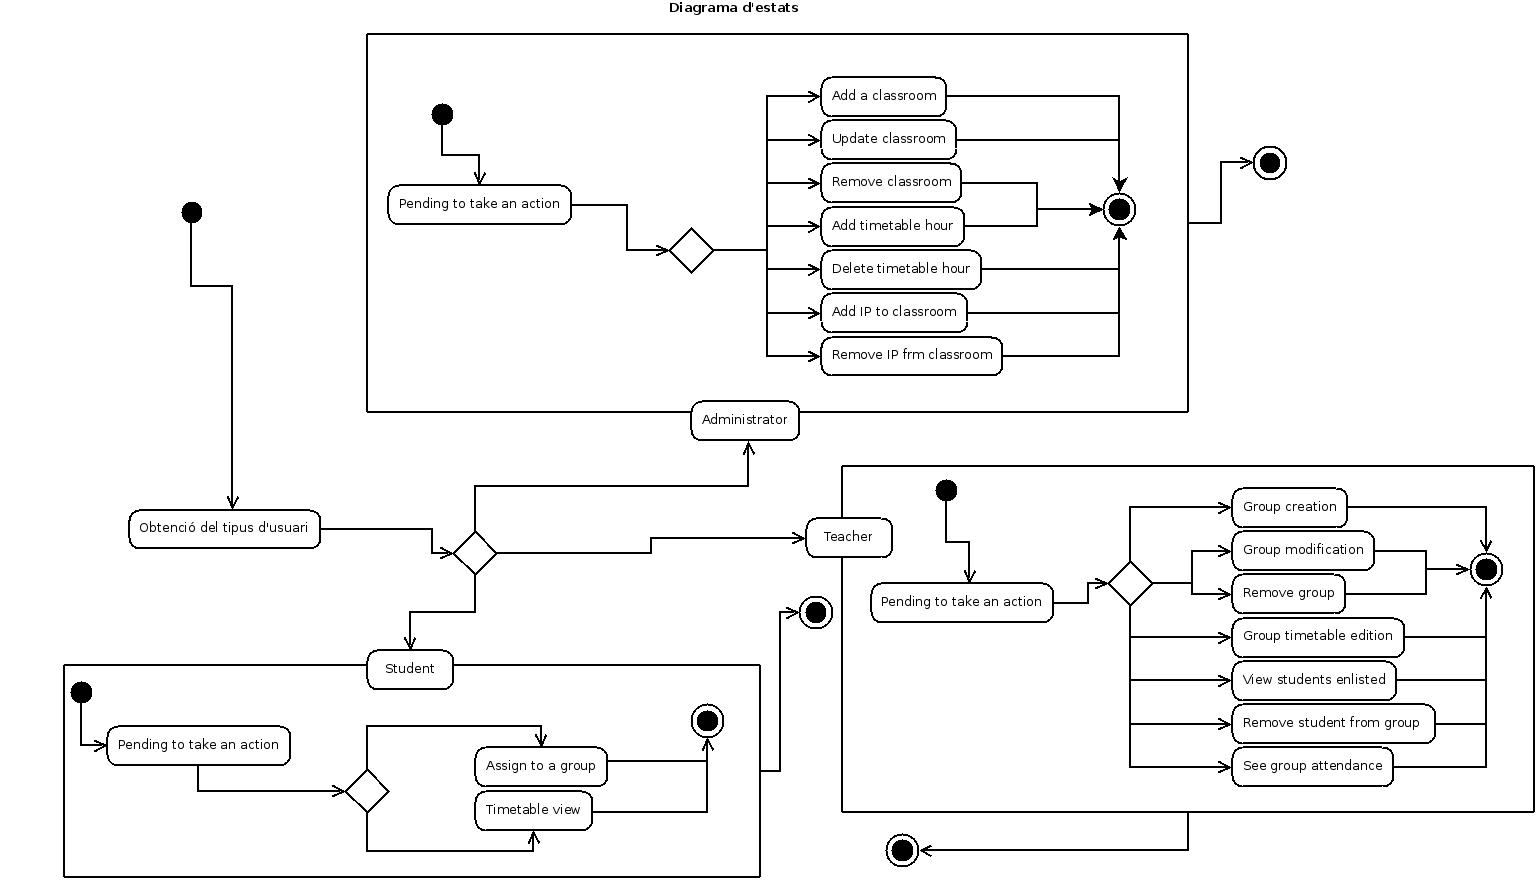
\includegraphics[width=14cm,keepaspectratio]{img/DiagramaEstats-rf.jpg}
		\caption[List caption]{Diagrama de estats del sistema.}
		\label{fig:DiagramaEstats-rf}
		\end{center}
		\end{figure}
\section{Interfície d'usuari}
Al capítol sobre el Manual de l'usuari d'aquesta documentació es trobaràn totes i cadascúna de les pantalles finals del sistema detallades.
\chapter{Evolució del projecte i decissions de disseny}
En aquest capítol es descriu la evolució que ha tingut el projecte aixi com també es descriuen els problemes que s'han anat trobant i com s'han resolt. 
Per comparar es mostren també dos diagrames de Gantt, un amb la previsió i idea inicial de com es repartiria la feina del projecte i un de final amb el que ha estat realment la evolució d'aquest amb les variacions que els problemes han provocat. 
\section{Previsió de l'evolució del projecte}
Inicialment es tenia prevista una evolució del projecte com segueix (Figura ~\ref{fig:GanttProject}).
		\begin{figure}[H] %Here overriding the specifications of Latex good placement
		\begin{center}
		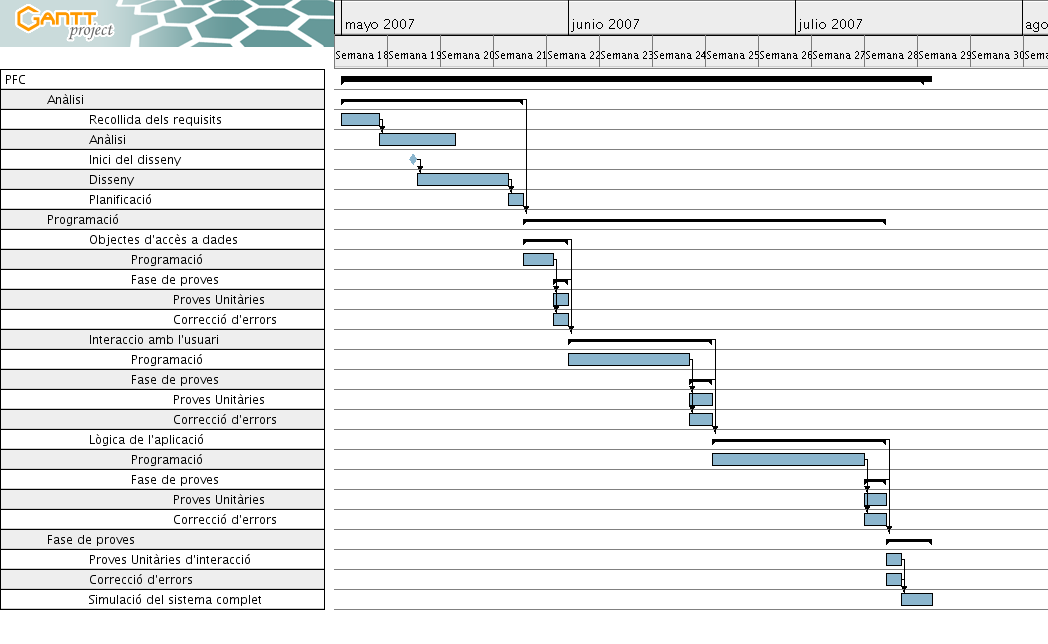
\includegraphics[width=0.90\textwidth,keepaspectratio]{img/GanttProject.png}
		\caption[List caption]{Previsió de l'evolució del projecte. Les unitats representades per les columnes són setmanes de treball.}
		\label{fig:GanttProject}
		\end{center}
		\end{figure}
\section{Evolució del projecte}
Partint de l'idea inicial del projecte, en aquesta secció presentem l'evolució real que ha tingut el projecte, els problemes trobats i les resolucions d'aquests problemes.
\subsection{Anàlisi}
En aquest moment del projecte es van plasmar els requisits essencials del projecte com eren la gestió de les aules, de les hores lectives, dels grups i dels horaris d'aquests grups per a cada curs.
Realment senzills si s'observa la primera revisió de l'especificació funcional.\\
Es va tenir que decidir, i per tant entendre, la diferencia entre Mòdul d'activitat i Block de Moodle per determinar quin dels dos tipus de plugins s'hauria de implementar. Es pot veure la definició en la secció d'introducció on s'intenten definir tots dos.\\
Bàsicament la diferència rau en què els mòduls d'activitat serveixen per interactuar amb els estudiants mitjançant activitats a nivell de temari que han de realitzar mitjançant les quals els professors poden avaluar o fer un seguiment dels coneixements assolits pels alumnes mentre que els blocs serveixen per mostrar informació adicional sobre els cursos o l'entorn i per tant es va escollir el Block per idoneïtat amb l'ús. Per poder començar i tenir una guía per poder començar amb el desenvolupament del block es va seguir la guía de desenvolupament que podem trobar a la següent adreça \url{http://docs.moodle.org/en/Development:Blocks}.\\
Els següents subpunts defineixen com es van abordar i com s'implementen certes solucions mitjançant les eines que aporten la plataforma Moodle.\\
\subsubsection{Base de dades}\label{AnalisiBasededades}
En versions anteriors a la 1.7 la creació de les taules en bases de dades es feia mitjançant scripts SQL, tants scripts com per Sistemes Gestors de Bases de Dades es volia fer compatible el nou mòdul. A partir de la versió 1.7 es fa mitjançant fitxers xmldb, uns fitxers xml pensats per la creació de bases de dades (Veure secció \ref{annexxmldb}, pàgina \pageref{annexxmldb} ). Es redueix llavors la creació de les taules de la base de dades a un sol fitxer que el sistema Moodle interpreta per cadascúna de les base de dades amb les que pot treballar.
\begin{lstlisting}[style=SQL, caption=Sentències SQL equivalents al fitxer xmldb per la creació de les taules]
CREATE TABLE mdl_timetable ( 
  id bigint(10) unsigned NOT NULL auto_increment, 
  instanceid bigint(10) unsigned NOT NULL, 
  courseid bigint(10) NOT NULL, 
  `name` varchar(255) default NULL, 
  PRIMARY KEY  (id), 
  UNIQUE KEY mdl_time_ins_uix (instanceid), 
  KEY mdl_time_cou_ix (courseid) 
); 


CREATE TABLE mdl_timetable_classroom ( 
  id bigint(10) unsigned NOT NULL auto_increment, 
  capacity bigint(10) unsigned NOT NULL, 
  `name` varchar(255) NOT NULL default '', 
  PRIMARY KEY  (id) 
); 


CREATE TABLE mdl_timetable_classroomip ( 
  id bigint(10) unsigned NOT NULL auto_increment, 
  classroomid bigint(10) unsigned NOT NULL, 
  ip varchar(15) NOT NULL, 
  PRIMARY KEY  (id), 
  UNIQUE KEY mdl_timeclas_claip_uix (classroomid,ip), 
  KEY mdl_timeclas_cla_ix (classroomid) 
); 


CREATE TABLE mdl_timetable_classroomip_log ( 
  id bigint(10) unsigned NOT NULL auto_increment, 
  hourtable_log_id bigint(10) NOT NULL, 
  ip varchar(15) NOT NULL, 
  PRIMARY KEY  (id), 
  UNIQUE KEY mdl_timeclaslog_houip_uix (hourtable_log_id,ip) 
); 


CREATE TABLE mdl_timetable_group ( 
  id bigint(10) unsigned NOT NULL auto_increment, 
  timetableid bigint(10) NOT NULL, 
  studentsnumber bigint(10) unsigned default NULL, 
  changeallowed tinyint(1) default NULL, 
  commongroup tinyint(1) default NULL, 
  `name` varchar(255) default NULL, 
  PRIMARY KEY  (id), 
  KEY mdl_timegrou_tim_ix (timetableid) 
); 


CREATE TABLE mdl_timetable_hours ( 
  id bigint(10) unsigned NOT NULL auto_increment, 
  starthour varchar(5) NOT NULL, 
  endhour varchar(5) NOT NULL, 
  PRIMARY KEY  (id), 
  UNIQUE KEY mdl_timehour_staend_uix (starthour,endhour) 
); 


CREATE TABLE mdl_timetable_hourtable ( 
  id bigint(10) unsigned NOT NULL auto_increment, 
  starthour varchar(5) NOT NULL, 
  weekday varchar(1) NOT NULL, 
  classroomid bigint(10) NOT NULL, 
  endhour varchar(5) NOT NULL, 
  groupid bigint(10) NOT NULL, 
  `name` varchar(255) default NULL, 
  PRIMARY KEY  (id), 
  UNIQUE KEY mdl_timehour_staweegroclae_uix (starthour,weekday,groupid,classroomid,endhour), 
  KEY mdl_timehour_staend_ix (starthour,endhour), 
  KEY mdl_timehour_cla_ix (classroomid), 
  KEY mdl_timehour_gro_ix (groupid) 
); 


CREATE TABLE mdl_timetable_hourtable_log ( 
  id bigint(10) unsigned NOT NULL auto_increment, 
  starthour varchar(5) NOT NULL, 
  weekday varchar(1) NOT NULL, 
  classroomid bigint(10) NOT NULL, 
  endhour varchar(5) NOT NULL, 
  groupid bigint(10) NOT NULL, 
  `name` varchar(255) default NULL, 
  `data` varchar(10) NOT NULL, 
  PRIMARY KEY  (id), 
  UNIQUE KEY mdl_timehourlog_staweegroc_uix (starthour,weekday,groupid,classroomid,endhour,`data`) 
); 


CREATE TABLE mdl_timetable_users ( 
  id bigint(10) unsigned NOT NULL auto_increment, 
  groupid bigint(10) NOT NULL, 
  userid bigint(10) NOT NULL, 
  PRIMARY KEY  (id), 
  UNIQUE KEY mdl_timeuser_grouse_uix (groupid,userid), 
  KEY mdl_timeuser_gro_ix (groupid), 
  KEY mdl_timeuser_use_ix (userid) 
);
\end{lstlisting}
Les versions dels fitxers xmldb equivalents a aquest script SQL de creació de taules els podem trobar a ambdues especificacions funcionals (secció \ref{xmldb-1r}, pàgina \pageref{xmldb-1r}  i secció \ref{xmldb-rf}, pàgina \pageref{xmldb-rf} )
\subsubsection{Rols d'usuari}\label{AnalisiRolsdUsuari}
El identificador d'usuari i l'identificador de course s’obtindran del sistema. 
Es informació que s’obtindrà de Moodle, de les taules d’usuari i de curs respectivament. 
Obtenció de la informació dels usuaris 
A tenir en compte els camps següents (extret de la pròpia base de dades):
\begin{center}
   \begin{tabular}{| l | l |}
     \hline \multicolumn{2}{|>{\columncolor[gray]{.8}}c|}{mdl\_user}\\
     \hline \rowcolor[gray]{.5}Camp & Tipus\\
     \hline \multicolumn{2}{|c|}{(...)}\\ 
     \hline id & bigint(10)\\ 
     \hline \multicolumn{2}{|c|}{(...)}\\
	  \hline username & varchar(100)\\ 
	  \hline	firstname & varchar(100)\\ 
	  \hline lastname & varchar(100)\\ 
     \hline \multicolumn{2}{|c|}{(...)}\\
	  \hline
   \end{tabular}
\end{center}

Els valors dels usuaris s'obtenen a partir de una de les variables globals de Moodle \$USER (Veure secció \ref{annexvariablesglobals}, pàgina \pageref{annexvariablesglobals} )

El model d'interacció dependrà del tipus d'usuari, que Moodle determina a través dels rols. Per determinar en cada moment quin tipus d'usuari és el  que entra al 	sistema es pot consultar el seu rol mitjançant les funcions:
\begin{center}
   \begin{tabular}{l}
		isadmin()\\
		isteacher()\\
		isstudent()\\
   \end{tabular}
\end{center}
Un exemple de la seva utilització:
\begin{lstlisting}[style=PHP, caption=Exemple de comprovació de rol d'usuari en versions de Moodle anteriors a la 1.7,escapechar=\%]
require_login($courseid);
if (isteacher($courseid) && confirm_sesskey($sesskey))
{ 
/*Accions (validaci%\color{gray45}ó%, confirmaci%\color{gray45}ó%, guardar a bbdd, etc., depenent de la p%\color{gray45}à%gina que sigui)*/
}else{
/*Redirigeixo a p%\color{gray45}à%gina del curs*/
}  
\end{lstlisting}

Això però es feia aixi en versions de Moodle anterios a la 1.7. Per permetre una millor flexibilitat en la definició dels rols això ha canviat i en la documentació d'aquesta nova versió s'especifica un nou funcionament per definir funcionalitats depenent del rol (Veure secció \ref{annexrols}, pàgina \pageref{annexrols} ). Així, ara si es vol definir una funcionalitat accessible o no depenent del rol es defineix el nom de la funcionalitat i per cadascún dels rols el nivell de seguretat que se li vol dónar i al codificar es farà ús de la funció \textsl{has\_capability}

Aqui hi ha un exemple de la nova manera d'obtenir els rols per un millor enteniment:
\begin{lstlisting}[style=PHP, caption=Fitxer access.db]
<?php

$mod_prueba_capabilities = array(

'mod/prueba:mostrar_hola_profesor' => array(

'captype' => 'write',
'contextlevel' => CONTEXT_MODULE,
'legacy' => array(
'editingteacher' => CAP_PROHIBIT,
'coursecreator' => CAP_PROHIBIT,
'teacher' => CAP_ALLOW,
'student' => CAP_PROHIBIT,
'admin' => CAP_PROHIBIT
)
),

'mod/prueba:mostrar_hola_alumno' => array(

'captype' => 'write',
'contextlevel' => CONTEXT_MODULE,
'legacy' => array(
'teacher' => CAP_PROHIBIT,
'editingteacher' => CAP_PROHIBIT,
'coursecreator' => CAP_PROHIBIT,
'admin' => CAP_ALLOW,
'student' => CAP_PROHIBIT
)
)
);

?>
\end{lstlisting}
\begin{lstlisting}[style=PHP, caption=Fitxer view.php]
(...)
/// Print the main part of the page

$context = get_context_instance(CONTEXT_MODULE, $cm->id);

if (has_capability( 'mod/prueba:mostrar_hola_profesor', $context)) {
echo 'Hola profesor';
}
else if(has_capability('mod/prueba:mostrar_hola_alumno',$context)){ 
echo 'Hola alumno';
} 
\end{lstlisting}
\subsubsection{Interfície d'usuari}
Degut a que depenent dels rols assignats a l'usuari pot realitzar diferents funcionalitats del bloc, s'han implementat les pantalles mitjançant un sistema de pestanyes, on en cadascúna d'elles s'hi pot realitzar la funcionalitat corresponent. Per cada usuari només es mostraran les pestanyes les cuals permeten l'accès a la funcionalitat aplicada al rol. \\
En la primera revisió de l'especificació funcional hi ha un apartat per la interfície d'usuari on hi han uns primers esboços del que es volia presentar per a cada pantalla. \\
En la revisió final de l'especificació funcional no hi ha un apartat concret per a la interfície d'usuari ja que en el capítol dedicat al manual de l'usuari es detallen totes i cadascúna de les pantalles que s'han implementat finalment.\\
\subsubsection{Disseny. Model implementat.}
Per evitar que el codi es dividis únicament en fitxers .php, on cadascún d'ells tingués tota la lògica i els elements de representació per pantalla 	mitjançant un codi poc estructurat i que fós dificil de seguir s'ha dissenyat un sistema que permet simular un senzill sistema amb el patró Model-Vista-Controlador (Figura ~\ref{fig:DiagramaMyMVC}) dins la estructura que Moodle obliga a seguir per implementar blocks. \\
Cadascúna de les accions que es poden prendre tenen un nom únic que la diferència de la resta. Aquest mateix nóm serà el que tindràn els fitxers .php que realment realitzen les operació per poder executar l'acció, i el nom del fitxer .html que finalment es qui mostra els resultats.\\
		\begin{figure}[H] %Here overriding the specifications of Latex good placement
		\begin{center}
		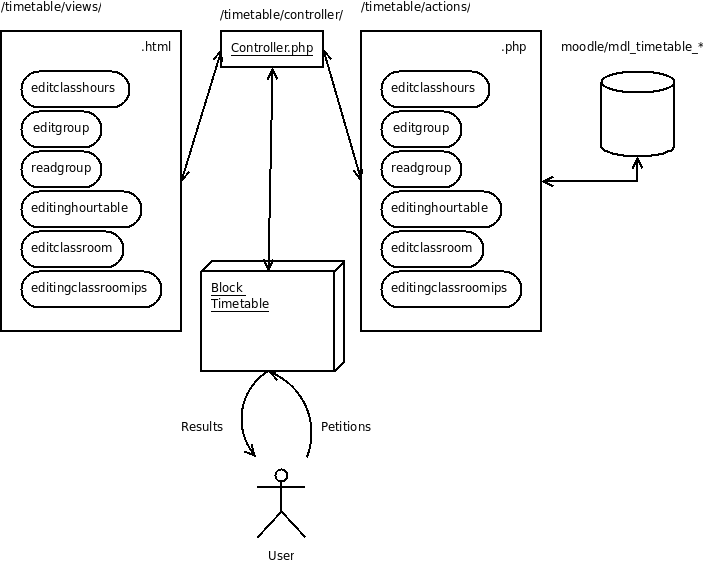
\includegraphics[width=0.90\textwidth,keepaspectratio]{img/DiagramaMyMVC.png}
		\caption[List caption]{Esquema del model d'implementació.}
		\label{fig:DiagramaMyMVC}
		\end{center}
		\end{figure}

\subsubsection{Control de l'assistència}
Es va concretar posteriorment que faria falta també una opció per al professorat per poder controlar l'assistència dels alumnes a les classes.\\
El sistema Moodle ja emmagatzema les dades d'accès a l'entorn en una taula anomenada mdl\_log, on es guarda l'usuari, el moment en que realitza l'acció, l'acció que ha realitzat i l'adreça IP desde que s'ha realitzat. Per tant només faria falta creuar aquestes dades amb les hores de classe de cada grup, per mostrar per cadascún d'ells si l'accès s'ha produit desde una adreça IP de les quals l'administrador sap que serà una adreça de l'aula en que es realitza aquella hora de classe.\\
El problema que hi ha es que les classes són elements vius que es poden canviar en qualsevol moment del curs de manera que la taula on s'emmagatzemen les dades de les classes per cada grup no serveix per creuar les dades amb els registres de la taula mdl\_log. Per tant, s'ha d'utilitzar una taula (timetable\_hourtable\_log) per enregistrar l'històric de les classes que ja s'han efectuat, ja que si hi ha programada una classe per algun dia concret de la setmana i just abans es canvia aquesta no ha d'apareixer a la taula històrica perquè aquesta classe no s'ha arribat a solucionar.\\
Per cadascúna de les classes emmagatzemades en l'històric també ens interessa saber quines adreces IP eren vàlides en aquell moment per aquella aula, ja que també poden ser modificades. Això ho emmagatzemarem a la taula (timetable\_classroomip\_log). \\
La solució que s'ha emprat es utilitzant un recurs que ens facilita Moodle \url{http://docs.moodle.org/es/Cron}. \\
Quan s'implementen els mòduls o els blocs hi ha l'opció d'implementar una funció que serà executada quan es faci una crida a \url{http://servidorexemple.com/moodle/admin/cron.php}. Aquesta funció és en el cas dels mòduls una funció nommodul\_cron() dins el fitxer nommodul/lib.php i en el cas dels blocks una funció cron() dins el fitxer nomblock/block\_nomblock.php. Es pot consultar això dins la documentació de Moodle a la següent adreça \url{http://docs.moodle.org/en/Cron#Script_overview}.\\
Per tant, tal com diu la documentació de Moodle, s'haurà de programar una visita al script del Cron però si es vol que realment funcioni aquest script per emmagatzemar les classes realitzades correctament, és molt important que s'assegui que aquest script s'executa almenys un cop durant el moment en que s'estigui realitzant la classe.\\
\subsubsection{Flexibilitat amb la configuració del calendari de Moodle}
Moodle permet configurar el primer dia de la setmana i els dies que es consideren cap de setmana desde la secció calendari,a l'apartat Aparença de l'Administració del lloc (Figura ~\ref{fig:AdministracioCalendari}).\\
		\begin{figure}[H] %Here overriding the specifications of Latex good placement
		\begin{center}
		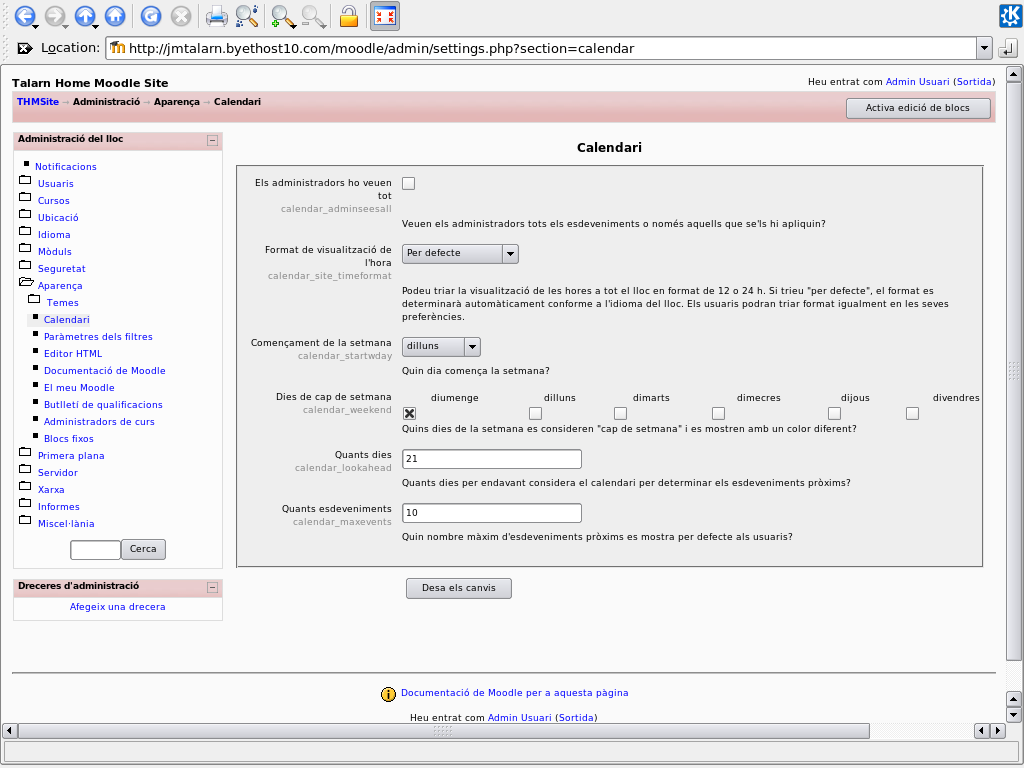
\includegraphics[width=12cm,height=10cm]{img/AdministracioCalendari.png}
		\caption[List caption]{Administració del lloc, Aparença, Calendari.}
		\label{fig:AdministracioCalendari}
		\end{center}
		\end{figure}
Aquest block està construit de manera que sempre consulta amb Moodle aquestes dades mitjançant les facilitats que ens proporciona la llibreria calendar.
\begin{lstlisting}[style=PHP,caption=Importació de la llibreria PHP necessària per manegar les  dades del calendari.]
	require_once($CFG->dirroot.'/calendar/lib.php');  
\end{lstlisting}
Per tant qualsevol canvi en qualsevol moment serà considerat a l'hora de representar els horaris dels alumnes.\\	
En el codi s'utilitza la següent iteració per recorrer els dies de la setmana i treballar amb ells amb l'ordre que s'ha establert a la configuració de Moodle.
\begin{lstlisting}[style=PHP,caption=Iteració per recorrer i processar els dies de la setmana en l'ordre definit per la configuració.]
	for($i = $display->minwday; $i <= $display->maxwday; ++$i)
\end{lstlisting}
Dins la llibreria del calendar aquests objecte \$display defineix els seus atributs minwday i maxwday com segueix:
\begin{lstlisting}[style=PHP,caption=calendar\textbackslash lib.php Definició del objecte display.]
    $display = &New stdClass;
    $display->minwday = get_user_preferences('calendar_startwday', CALENDAR_STARTING_WEEKDAY);
    $display->maxwday = $display->minwday + 6;
\end{lstlisting}
Per comprovar si es tracta d'un dia de cap de setmana s'utilitza la següent instrucció
\begin{lstlisting}[style=PHP,caption=Iteració per recorrer i processar els dies de la setmana en l'ordre definit per la configuració.]
	if(CALENDAR_WEEKEND & (1 << ($i % 7))) 
\end{lstlisting}
Aquesta constant CALENDAR\_WEEKEND es definida aixi:
\begin{lstlisting}[style=PHP,caption=calendar\textbackslash lib.php Definició de la constant CALENDAR\_WEEKEND.]
// This is a packed bitfield: day X is "weekend" if $field & (1 << X) is true
// Default value = 65 = 64 + 1 = 2^6 + 2^0 = Saturday & Sunday
define('CALENDAR_DEFAULT_WEEKEND',            65);
\end{lstlisting}
I per obtenir el literal associat al valor del dia setmanal s'utilitza la crida habitual per obtenir literals el fitxer de llenguatge apropiat. 
\begin{lstlisting}[style=PHP,caption=Crida per obtenir els literals per als noms dels dies de la setmana]
get_string($CALENDARDAYS[$i % 7], 'calendar')
\end{lstlisting}

\subsubsection{Internacionalització i ajuda}
Timetable ha estat traduït o almenys s'ha intentat que els literals i els fitxers d'ajuda siguin comprensibles en els següents idiomes: català, castellà, anglès i francès.\\
Moodle està pensat per poder ser utilitzat i traduït al màxim nombre de llengües possibles.\\ 
Qualsevol persona pot col·laborar en aquestes traduccions o fer petites modificacions per a ús local tal i com s'indica a la següent adreça \url{http://docs.moodle.org/ca/Traducci%C3%B3}.\\
En aquesta pàgina també indica com, a banda de col·laborar amb els traduccions en paquets de llenguatge generals de Moodle, col·laborar també amb les traduccions de mòduls i plugins de tercers. 
Aquestes instruccions serveixen per crear també els fitxers d'idioma per a nous mòduls i plugins.\\
Al mateix temps, però, s'han afegit també uns fitxers d'ajuda en format html i les seves traduccions. 
Per què siguin accessibles amb les mateixes condicions que la resta de fitxers d'ajuda del sistema, aquest contingut s'ha de copiar a la carpeta lang/XX\_utf8/help/nomdelbloc/  però de Moodle en comptes de la pròpia del component. on XX\_utf8 és el llenguatge éscollit per la traducció i nomdelbloc és el nom del bloc, en el nostre cas ca, es, en i fr per els idiomes i timetable com a nom.
Copiant aquests fitxers d'ajuda a la ruta especificada ens permet poder cridar-los amb la funció helpbutton, mostrant-se amb l'idioma corresponent.
\begin{lstlisting}[style=PHP,caption=Crida als fitxers d'ajuda on \$currenttab és el nom del fitxer.]
helpbutton($currenttab, get_string('help', 'block_timetable'), "timetable", true, true);
\end{lstlisting}
Aquesta instrucció obre la informació de l'ajuda en una finestra apart, què és el comportament habitual a l'hora de mostrar l'ajuda dins de Moodle.

\subsubsection{Versió de Moodle}\label{VersioMoodle}	
Al moment de començar aquest projecte no és volia fixar una versió mínima de Moodle però les millores i la solventació d'alguns defectes, gràcies a les col·laboracions dels desenvolupadors en algunes de les progressives versions versions han obligat a fixar una versió mínima.
En un principi és va començar a desenvolupar amb la versió 1.6 de Moodle.
A l'hora de consultar informació de com crear les taules de la base de dades, es va consultar la informació existent sobre la creació del fitxer xmldb () (Secció \ref{AnalisiBasededades}, pàgina \pageref{AnalisiBasededades} ). Es va escollir que la creació de la base de dades es faria amb aquest fitxer.\\
També, al consultar com es gestionen els rols a Moodle. És va trobar la documentació referent al tema de la versió 1.7 en la que comenta que s'utilitza un fitxer php per gestionar els permisos dels rols d'usuari (Secció \ref{AnalisiRolsdUsuari}, pàgina \pageref{AnalisiRolsdUsuari}).
Al escollir aquesta manera de gestionar aquests factors es va fixar per el moment la versió 1.7 de Moodle.
Més endavavant, durant el desenvolupament del projecte es va trobar un problema amb el registre d'usuaris, adreça IP i moment en que es realitzen les accions sobre el sistema  que es va sol·lucionar a la versió 1.8 de Moodle (Secció \ref{DesenvolupamentFuncioTime}, pàgina \pageref{DesenvolupamentFuncioTime}). Aquest problema afectava directament el projecte i es va forçar a versió mínima la 1.8 de Moodle.

\subsection{Programació}
\subsubsection{Objectes d'accès a dades}
En un principi es va pensar que s'hauria d'implementar una capa per facilitar l'accès a les dades, mitjançant unes classes que accedirien a la base de dades per recuperar cadascuna de les instàncies necessàries per gestionar les dades.
Moodle en aquest cas ens facilita les coses i ja incorpora les funcions necessàries per recuperar dades de la base de dades i mapejar-les sobre objectes amb camps corresponents a les columnes amb el mateix nom. En cas de recuperar de la base de dades un conjunt de registres i no només un de sol aquestes funcions ja recuperen una array d'aquests objectes.
Dins la llibreria dmllib.php podem trobar totes les funcions necessàries per poder accedir a la base de dades d'una manera transparent al usuari (Veure secció \ref{annexaccesdades}, pàgina \pageref{annexaccesdades} ).

\subsubsection{Interacció amb l'usuari i Lògica de l'aplicació}
A l'hora de seguir amb la implementació de l'aplicació  es va canviar el plantejament inicial realitzat en la previsió inicial (Figura ~\ref{fig:GanttProject}) del desenvolupament del projecte de implementar primer tota la part d'interacció amb l'usuari i després tota la lògica de la aplicació per el desenvolupament de cadascúna de les accions que es poden realitzar. 
És a dir, en comptes de subdividir la tasca de la programació amb subtasques per la lògica i subtasques per l'interfície es va optar per subdividir-ho amb subtasques per cadascúna de les accions que es poden prendre dins el sistema. Tal com mostra el diagrama (Figura ~\ref{fig:GanttProjectProgramacio}) de la següent manera:
		\begin{figure}[H] %Here overriding the specifications of Latex good placement
		\begin{center}
		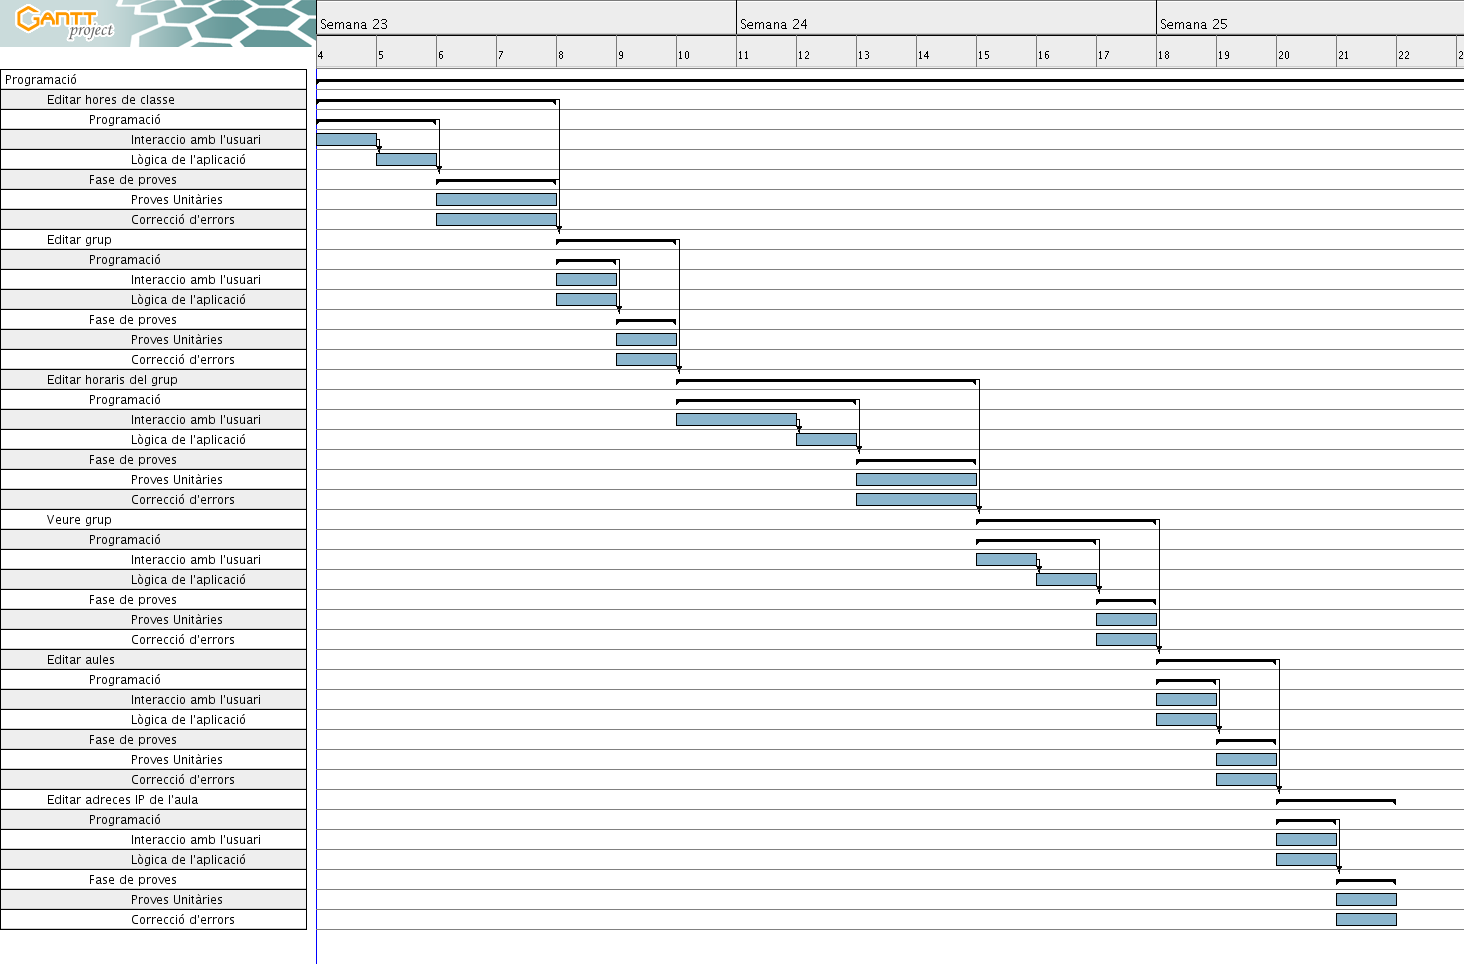
\includegraphics[width=0.90\textwidth,keepaspectratio]{img/GanttProjectProgramacio.png}
		\caption[List caption]{Evolució en el desenvolupament de la programació del projecte.}
		\label{fig:GanttProjectProgramacio}
		\end{center}
		\end{figure}

\subsection{Fase de proves. Problemes i resolució.}
Tant en la fase de proves (fase final de la planificació), com en cadascúna de les subfases de Proves unitàries dins el desenvolupament, a part d'errors comuns de programació, s'han anat trobat diferent problemes, i s'han solucionat tal com s'esmenta en els apartats següents.
\subsubsection{Taules amb camp Id}
Un dels primers problemes en que varem trobar es que algunes de les taules com ara mdl\_timetable\_hourtable, on es guarden les hores de classe per cada dia de la setmana per cada grup, o la taula mdl\_timetable\_hours, on es guarden unicament les hores en que es fa classe, o la taula mdl\_timetable\_classroomip, on es guarda la relació entre les adreces IP vàlides i les aules corresponents; s'havien dissenyat sense un camp concret que ens servís d'identificador de clau primaria de la taula ja que no era un camp sol el que determinaria la clau primaria si no un conjunt (hora d'inici, dia de la setmana, identificador del grup i identificador de l'aula per mdl\_timetable\_hourtable, en mdl\_timetable\_hours unicament es guarda l'hora d'inici i la hora de fi per cada possible classe i la relació entre adreces IP i aules nomès hauria de guardar l'adreça IP i l'identificador de l'aula).
Això suposa un problema si s'utilitzen les funcions que dòna l'entorn ja que es suposa que totes les taules han de tenir un camp anomenat id, que serveixi de clau primària. 
Es pot trobar una discussió sobre el tema als forums de Moodle: \url{http://moodle.org/mod/forum/discuss.php?d=38183#p176751} 
\url{http://docs.moodle.org/en/IdColumnReasons} (Veure secció \ref{annexcampid}, pàgina \pageref{annexcampid} )
En els debat sobre el tema es fa referència a un paràmetre dins la funció per per indicar quina és el camp clau de la taula. Però tal com es pot observar en la pròpia definició d'aquesta funció és un parametre $"$obsolet$"$ i n'ignora el seu ús.

%\begin{lstlisting}[style=PHP]
\begin{tt}
\begin{center}
 	\begin{tabular}{| p{12cm} |}
	\hline
	\rowcolor[gray]{0.5}insert\_record(\$table, \$dataobject, \$returnid=true, \$primarykey='id') X-Ref\\
	Insert a record into a table and return the $"$id$"$ field if required\\
	\hline \\
	If the return ID isn't required, then this just reports success as true/false.\\
	\$dataobject is an object containing needed data\\
	\\
	param: string \$table The database table to be checked against.\\
	param: object \$dataobject A data object with values for one or more fields in the record\\
	param: bool \$returnid Should the id of the newly created record entry be returned? If this option is not requested then true/false is returned.\\
	param: string \$primarykey (obsolete) This is now forced to be 'id'. \\
	\hline
	\end{tabular}
\end{center}	
\end{tt}	
%\end{lstlisting}
Per tant s'ha hagut d'afegir a aquestes taules un camp anomenat id i declarar-lo com a clau primaria.

\subsubsection{Funció time() i zones horàries}\label{DesenvolupamentFuncioTime}
Per el desenvolupament del control de l'assistència es va crear un sistema que crea les dades de les classes realitzades amb les dades que ja emmagatzema Moodle a la taula mdl\_log.\\
Moodle guarda en aquesta taula la informació de les accions que es prenen sobre Moodle, l'adreça IP i el moment, un timestamp, en que es realitzen.\\
En les primeres proves això es va provar en un servidor montat en la mateixa màquina on es desenvolupava i es provava i no va suposar cap problema. 
Però més endavant és va provar en un servidor Moodle montat sobre un servidor de hosting gratuit situat a Nova York, mentre que la configuració de Moodle constava que el servidor havia de mostrar l'hora de fus hoari GMT +1. Aquesta diferència interferia en el camp time que s'emmagatzema a la taula mdl\_log, ja que la instrucció que obtenia el timestamp i l'emmagatzemava era errònia. \\
Aquest error i la seva resolució es pot veure com va ser discutit a la següent adreça \url{http://tracker.moodle.org/browse/MDL-13959} on es pot observar a part de l'error comentat com aclareix com s'han d'utilitzar les funcions per obtenir un timestamp correcte per al moment necessari (Veure secció \ref{annexfunciotime}, pàgina \pageref{annexfunciotime} ).\\

La resolució del problema amb la instrucció usergetdate() i els consells sobre la seva utilització ens porten a utilitzar-la com segueix:\\
\begin{lstlisting}[style=PHP]
	$now3 = usergetdate(time());
\end{lstlisting}
Aquesta instrucció ens serveix per obtenir l'hora del usuari administrador, que per una correcta execució no hauria de ser diferent de la configuració de Moodle.\\
\subsubsection{Visualització del registre d'assistència}
A la pantalla de visualització del control d'assistència dels alumnes per un grup, si els registres retornats de les classes realitzades per aquell grup eren una quantitat força alta, és a dir, que per aquell grup i les dates seleccionades hi havien força classes realitzades, les dades marxaven de la finestra, obligant a l'usuari a utilitzar la barra de desplaçament horitzontal del navegador web, perdent de vista aixi la resta de dades del grup, com ara la llista de alumnes o les dates en que s'ha fet la consulta.\\
Per evitar això, per la representació de les dades s'ha obtat per jugar amb els estils de les capes dins de l'html forçant aixi que les dades si ocupen més espai que el reservat amb el <div>, aquesta capa mostri la barra de desplaçament i no sigui el navegador web el que la mostri.
\begin{lstlisting}[style=HTML, caption=codi de readgroup.html\, on es juga amb els estils de les capes per mostrar la barra de desplaçament horitzontal.]
 <div id="tablaLogs" >
 	<div id="Layer1" style="position:relative;float:left;">
 		<!-- Pinta una taula amb la llista d'usuaris-->
	</div>

	<div id="Layer1" style="position:relative;width:80%;overflow:auto;float:left;">
		<!-- Pinta la taula de la llista de classes, on les files seran els
			 accessos dels usuaris amb IP i les columnes les classes realizades--> 
   </div>
 </div> <!--TablaLogs"-->

\end{lstlisting}

\chapter{Guia d'insta\l.lació}
El procés d'insta\l.lació és l'habitual dels blocs de Moodle:\\ 
\url{http://moodle.org/mod/forum/discuss.php?d=38783},\\ 
\url{http://docs.moodle.org/en/Installing_contributed_modules_or_plugins}.\\
S'haurà de copiar la carpeta timetable dins la carpeta blocks allà on correspongui, segons la insta\l.lació de Moodle.
S'haurà d'accedir com l'usuari administrador del lloc (normalment admin) e insta\l.lar el bloc clicant a Notificacions dins el bloc d'Administració del lloc.\\
Posteriorment es mostrarà la informació corresponent a la correcta creació de les taules, tal com es mostra a les següents linies:
\begin{lstlisting}[style=SQL, caption=Resultat de la insta\l.lació del Block dins al sistema Moodle,escapechar=\%]
No warnings - Scroll to the continue button
timetable

(mysql): SHOW TABLES

(mysql): SHOW TABLES

(mysql): SHOW TABLES

(mysql): SHOW TABLES

(mysql): SHOW TABLES

(mysql): SHOW TABLES

(mysql): SHOW TABLES

(mysql): SHOW TABLES

(mysql): SHOW TABLES

(mysql): SHOW TABLES

(mysql): SHOW TABLES

(mysql): SHOW TABLES

(mysql): SHOW TABLES

(mysql): SHOW TABLES

(mysql): SHOW TABLES

(mysql): CREATE TABLE mdl_timetable_hours ( id BIGINT(10) unsigned NOT NULL auto_increment, starthour VARCHAR(5) NOT NULL DEFAULT '', endhour VARCHAR(5) NOT NULL DEFAULT '', CONSTRAINT PRIMARY KEY (id) )
%È%xit 

(mysql): ALTER TABLE mdl_timetable_hours COMMENT='timetable_hours table retrofitted from MySQL'
%È%xit

(mysql): CREATE UNIQUE INDEX mdl_timehour_staend_uix ON mdl_timetable_hours (starthour, endhour)
%È%xit

(mysql): CREATE TABLE mdl_timetable_classroom ( id BIGINT(10) unsigned NOT NULL auto_increment, capacity BIGINT(10) unsigned NOT NULL, name VARCHAR(255) NOT NULL DEFAULT '', CONSTRAINT PRIMARY KEY (id) )
%È%xit

(mysql): ALTER TABLE mdl_timetable_classroom COMMENT='timetable_classroom table retrofitted from MySQL'
%È%xit

(mysql): CREATE TABLE mdl_timetable ( id BIGINT(10) unsigned NOT NULL auto_increment, instanceid BIGINT(10) unsigned NOT NULL, courseid BIGINT(10) NOT NULL, name VARCHAR(255) DEFAULT NULL, CONSTRAINT PRIMARY KEY (id) )
%È%xit

(mysql): ALTER TABLE mdl_timetable COMMENT='timetable table retrofitted from MySQL'
%È%xit

(mysql): CREATE INDEX mdl_time_cou_ix ON mdl_timetable (courseid)
%È%xit

(mysql): CREATE UNIQUE INDEX mdl_time_ins_uix ON mdl_timetable (instanceid)
%È%xit

(mysql): CREATE TABLE mdl_timetable_group ( id BIGINT(10) unsigned NOT NULL auto_increment, timetableid BIGINT(10) NOT NULL, studentsnumber BIGINT(10) unsigned DEFAULT NULL, changeallowed TINYINT(1) DEFAULT NULL, commongroup TINYINT(1) DEFAULT NULL, name VARCHAR(255) DEFAULT NULL, CONSTRAINT PRIMARY KEY (id) )
%È%xit

(mysql): ALTER TABLE mdl_timetable_group COMMENT='timetable_group table retrofitted from MySQL'
%È%xit

(mysql): CREATE INDEX mdl_timegrou_tim_ix ON mdl_timetable_group (timetableid)
%È%xit

(mysql): CREATE TABLE mdl_timetable_users ( id BIGINT(10) unsigned NOT NULL auto_increment, groupid BIGINT(10) NOT NULL, userid BIGINT(10) NOT NULL, CONSTRAINT PRIMARY KEY (id) )
%È%xit

(mysql): ALTER TABLE mdl_timetable_users COMMENT='timetable_users table retrofitted from MySQL'
%È%xit

(mysql): CREATE UNIQUE INDEX mdl_timeuser_grouse_uix ON mdl_timetable_users (groupid, userid)
%È%xit

(mysql): CREATE INDEX mdl_timeuser_gro_ix ON mdl_timetable_users (groupid)
%È%xit

(mysql): CREATE INDEX mdl_timeuser_use_ix ON mdl_timetable_users (userid)
%È%xit

(mysql): CREATE TABLE mdl_timetable_hourtable ( id BIGINT(10) unsigned NOT NULL auto_increment, starthour VARCHAR(5) NOT NULL DEFAULT '', weekday VARCHAR(1) NOT NULL DEFAULT '', classroomid BIGINT(10) NOT NULL, endhour VARCHAR(5) NOT NULL DEFAULT '', groupid BIGINT(10) NOT NULL, name VARCHAR(255) DEFAULT NULL, CONSTRAINT PRIMARY KEY (id) )
%È%xit

(mysql): ALTER TABLE mdl_timetable_hourtable COMMENT='timetable_hourtable table retrofitted from MySQL'
%È%xit

(mysql): CREATE UNIQUE INDEX mdl_timehour_staweegroclae_uix ON mdl_timetable_hourtable (starthour, weekday, groupid, classroomid, endhour)
%È%xit

(mysql): CREATE INDEX mdl_timehour_staend_ix ON mdl_timetable_hourtable (starthour, endhour)
%È%xit

(mysql): CREATE INDEX mdl_timehour_cla_ix ON mdl_timetable_hourtable (classroomid)
%È%xit

(mysql): CREATE INDEX mdl_timehour_gro_ix ON mdl_timetable_hourtable (groupid)
%È%xit

(mysql): CREATE TABLE mdl_timetable_classroomip ( id BIGINT(10) unsigned NOT NULL auto_increment, classroomid BIGINT(10) unsigned NOT NULL, ip VARCHAR(15) NOT NULL DEFAULT '', CONSTRAINT PRIMARY KEY (id) )
%È%xit

(mysql): ALTER TABLE mdl_timetable_classroomip COMMENT='timetable_classroomip'
%È%xit

(mysql): CREATE UNIQUE INDEX mdl_timeclas_claip_uix ON mdl_timetable_classroomip (classroomid, ip)
%È%xit

(mysql): CREATE INDEX mdl_timeclas_cla_ix ON mdl_timetable_classroomip (classroomid)
%È%xit

(mysql): CREATE TABLE mdl_timetable_hourtable_log ( id BIGINT(10) unsigned NOT NULL auto_increment, starthour VARCHAR(5) NOT NULL DEFAULT '', weekday VARCHAR(1) NOT NULL DEFAULT '', classroomid BIGINT(10) NOT NULL, endhour VARCHAR(5) NOT NULL DEFAULT '', groupid BIGINT(10) NOT NULL, name VARCHAR(255) DEFAULT NULL, data VARCHAR(10) NOT NULL DEFAULT '', CONSTRAINT PRIMARY KEY (id) )
%È%xit

(mysql): ALTER TABLE mdl_timetable_hourtable_log COMMENT='timetable_hourtable_log
%È%xit

(mysql): CREATE UNIQUE INDEX mdl_timehourlog_staweegroc_uix ON mdl_timetable_hourtable_log (starthour, weekday, groupid, classroomid, endhour, data)
%È%xit

(mysql): CREATE TABLE mdl_timetable_classroomip_log ( id BIGINT(10) unsigned NOT NULL auto_increment, hourtable_log_id BIGINT(10) NOT NULL, ip VARCHAR(15) NOT NULL DEFAULT '', CONSTRAINT PRIMARY KEY (id) )
%È%xit

(mysql): ALTER TABLE mdl_timetable_classroomip_log COMMENT='timetable_classroomip_log'
%È%xit

(mysql): CREATE UNIQUE INDEX mdl_timeclaslog_houip_uix ON mdl_timetable_classroomip_log (hourtable_log_id, ip)
%\color{gray45}È%xit

S'han configurat correctament les taules Horari
\end{lstlisting}
Per últim si es vol accedir als fitxers d'ajuda, per qualsevol dels idiomes amb els quals s'han escrit aquests, i per simplificar aquest últim pas, s'haurà de copiar el contingut de la carpeta moodle/blocks/timetable/lang dins la carpeta moodle/lang sobreescrivint si s'escaigués els fitxers existents.\\
També és necessari que el cron s'estigui executant, configurat tal com indica la documentació de Moodle \url{http://docs.moodle.org/es/Cron}. La configuració és l'habitual però s'haurà de tenir en compte que si es vol que es guardi l'històric de 	classes realitzades el cron s'haurà d'executar almenys un cop durant la classe.\\
\begin{otherlanguage}{spanish}
\begin{quote}
La carga de este script no es muy alta, así que un intervalo de 5 minutos es razonable generalmente, pero si esto le preocupa, puede ampliar el periodo de tiempo a 15 minutos o incluso 30 minutos. Es mejor no establecer un intervalo de tiempo demasiado largo, ya que el retrasar el envío de mensajes de correo puede reducir la actividad del curso.
\end{quote}
\end{otherlanguage}
La documentació considera que 5 minuts es raonable, i es una bona configuració ja que es molt improbable que es programi una classe  de duració igual o inferior a 5 minuts. Tot i això si fos el cas de que s'haguessin programat classes de duració tant curta, només caldria reduir el temps entre execucions del cron perquè s'executes almenys un cop durant la classe.
Per saber quin és el funcionament del bloc consulteu el capítol de Manual d'usuari.
\chapter{Manual d'usuari}
\section{Introducció}
A partir de la visualització inicial del bloc, la pantalla es divideix aproximadament 	com segueix.
Cadascún dels usuaris, depenent del seu rol, tindrà accès a unes o altres opcions:\\
\begin{itemize}
\item Rol administrador (Figura ~\ref{fig:BlocProfileAdmin} i Figura ~\ref{fig:TabAdmin}):\\
\begin{figure}[H] %Here overriding the specifications of Latex good placement
\begin{center}
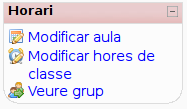
\includegraphics{img/BlocProfileAdmin.png}
\caption[List caption]{Aspecte del bloc per al rol administrador}
\label{fig:BlocProfileAdmin}
\end{center}
\end{figure}
\begin{figure}[H] %Here overriding the specifications of Latex good placement
\begin{center}
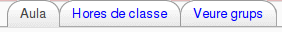
\includegraphics{img/TabAdmin.png}
\caption[List caption]{Pestanyes vistes per al rol administrador}
\label{fig:TabAdmin}
\end{center}
\end{figure}
\item Rol professor (Figura ~\ref{fig:BlocProfileTeacher} i Figura ~\ref{fig:TabTeacher}):\\
\begin{figure}[H] %Here overriding the specifications of Latex good placement
\begin{center}
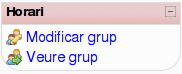
\includegraphics{img/BlocProfileTeacher.png}
\caption[List caption]{Aspecte del bloc per al rol professor}
\label{fig:BlocProfileTeacher}
\end{center}
\end{figure}

\begin{figure}[H] %Here overriding the specifications of Latex good placement
\begin{center}

\includegraphics{img/TabTeacher.png}
\caption[List caption]{Pestanyes vistes per al rol professor}
\label{fig:TabTeacher}
\end{center}
\end{figure}
\item Rol alumne (Figura ~\ref{fig:BlocProfileStudent} i Figura ~\ref{fig:TabStudent}):\\
\begin{figure}[H] %Here overriding the specifications of Latex good placement
\begin{center}
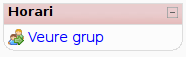
\includegraphics{img/BlocProfileStudent.png}
\caption[List caption]{Aspecte del bloc per al rol estudiant}
\label{fig:BlocProfileStudent}
\end{center}
\end{figure}
\begin{figure}[H] %Here overriding the specifications of Latex good placement
\begin{center}

\includegraphics{img/TabStudent.png}
\caption[List caption]{Pestanyes vistes per al rol estudiant}
\label{fig:TabStudent}
\end{center}
\end{figure}
\end{itemize}
Desde qualsevol de les pestanyes, a la dreta d'aquestes, es pot accedir a l'ajuda (Figura ~\ref{fig:WhereHelp}), 	un resum sense el detall gràfic d'aquest document Manual de l'usuari.
\begin{figure}[H] %Here overriding the specifications of Latex good placement
\begin{center}
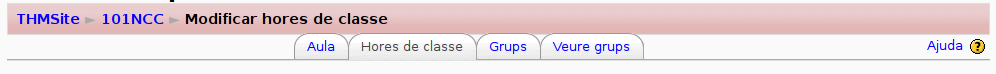
\includegraphics[width=0.90\textwidth,keepaspectratio]{img/WhereHelp.png}
\caption[List caption]{Situació de l'accès a l'ajuda}
\label{fig:WhereHelp}
\end{center}
\end{figure}
Si l'usuari està apuntat a algun grup i aquest grup té classes programades es mostrarà la informació de la pròxima classe del usuari com indica la figura (Figura ~\ref{fig:BlocIniciNextClass})
\begin{figure}[H] %Here overriding the specifications of Latex good placement
\begin{center}
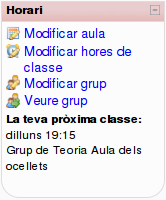
\includegraphics{img/BlocIniciNextClass.png}
\caption[List caption]{Si hi han classes programades per algun grup dels que està apuntat l'usuari es mostrarà la informació de la pròxima classe.}
\label{fig:BlocIniciNextClass}
\end{center}
\end{figure}

\section{Editant les aules}
Des d'aquesta pàgina (Figura ~\ref{fig:EditantAules}) pot afegir, modificar i eliminar les aules d'aquesta institució.
\begin{figure}[H] %Here overriding the specifications of Latex good placement
\begin{center}
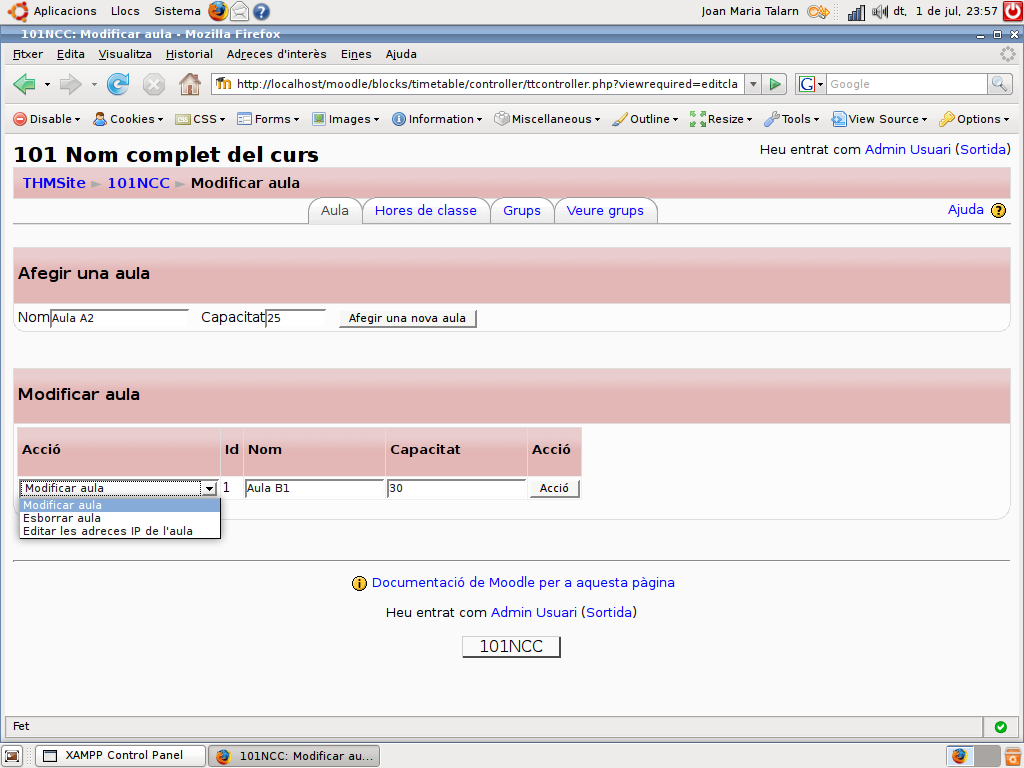
\includegraphics[height=10cm,width=12cm]{img/EditantAules.png}
\caption[List caption]{Pantalla per editar aules}
\label{fig:EditantAules}
\end{center}
\end{figure}

\begin{itemize}
\item\textbf{Afegir una aula} - des d'aquesta secció pot afegir una nova aula.
Només són necessaris dos paràmetres per afegir una nova aula:
	\begin{itemize}
	\item\textbf{nom} - el nom s'ultilitza per identificar cadascuna de les aules.
	\item\textbf{capacitat} - la màxima capacitat de les aules segons l'espai disponible.
	\end{itemize}
	
Si s'afegeix una aula i no s'ha introduït cap valor per la seva capacitat (Figura ~\ref{fig:AddAulaNoCapacity}), 
\begin{figure}[H] %Here overriding the specifications of Latex good placement
\begin{center}
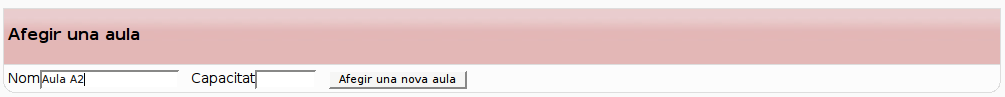
\includegraphics[width=16cm]{img/AddAulaNoCapacity.png}
\caption[List caption]{Afegint una aula sense indicar-hi la capacitat}
\label{fig:AddAulaNoCapacity}
\end{center}
\end{figure}

l'aula s'acaba afegint a la llista d'aules amb el valor 0 com a capacitat (Figura ~\ref{fig:AddAula0Capacity}).
\begin{figure}[H] %Here overriding the specifications of Latex good placement
\begin{center}
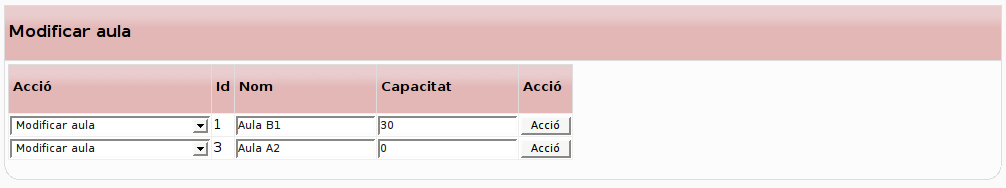
\includegraphics[width=16cm]{img/AddAula0Capacity.png}
\caption[List caption]{Aula creada amb capacitat 0}
\label{fig:AddAula0Capacity}
\end{center}
\end{figure}

I si s'afegeix una aula sense cap valor per al nom (Figura ~\ref{fig:AddAulaBlankName}), 
\begin{figure}[H] %Here overriding the specifications of Latex good placement
\begin{center}
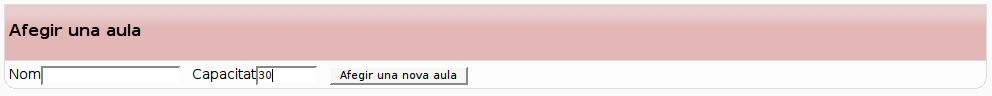
\includegraphics[width=16cm]{img/AddAulaBlankName.png}
\caption[List caption]{Afegir una aula sense indicar-hi cap nom}
\label{fig:AddAulaBlankName}
\end{center}
\end{figure}
l'aula s'acaba afegint sense cap valor al seu nom ja que s'identifica amb un identificador únic per a cada aula afegida (Figura ~\ref{fig:AddAulaNoName}).
\begin{figure}[H] %Here overriding the specifications of Latex good placement
\begin{center}
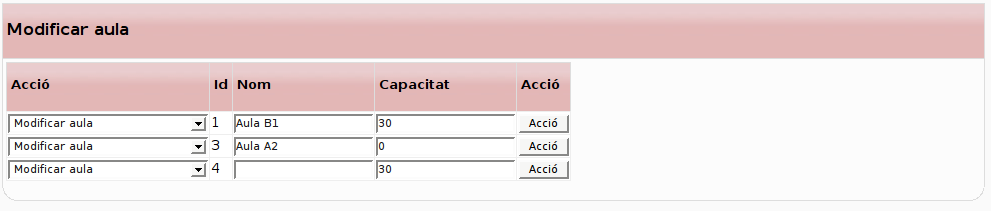
\includegraphics[width=16cm]{img/AddAulaNoName.png}
\caption[List caption]{Aula creada sense nom}
\label{fig:AddAulaNoName}
\end{center}
\end{figure}


\item\textbf{Editar aula} - des d'aquesta secció pot modificar o eliminar una aula que ja existeix.
Aquesta és una llista de totes les aules disponibles. Si no s'han afegit aules apareixerà un missatge mostrant que no hi han aules disponibles.
Es poden fer tres accions canviant el valor de la combo d'acció.
	\begin{itemize}
	\item\textbf{Actualitzar aula} - el nom i la capacitat poden ser modificats per cada fila de la llista però només pot ser actualitzat si aquesta acció és seleccionada a la combo d'acció i el botó d'acció és apretat.
	\item\textbf{Eliminar aula} - l'aula pot ser eliminada si aquesta acció és seleccionada i el botó d'acció és apretat. Una pantalla com la següent (Figura ~\ref{fig:EsborrarAula}) li demanarà que confirmi l'acció.
		\begin{figure}[H] %Here overriding the specifications of Latex good placement
		\begin{center}
		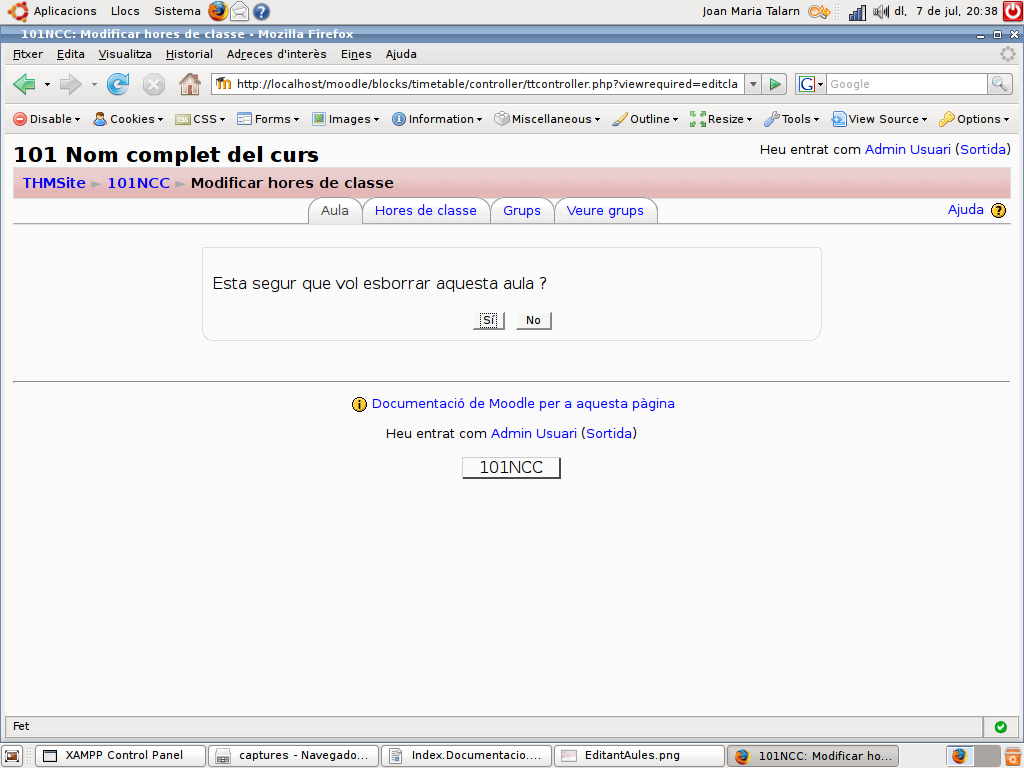
\includegraphics[height=10cm,width=12cm]{img/EsborrarAula.png}
		\caption[List caption]{Confirmació per esborrar una aula.}
		\label{fig:EsborrarAula}
		\end{center}
		\end{figure}
	\item\textbf{Editar les adreces IP de l'aula} - amb aquesta opció es podràn gestionar les adreces IP vàlides per cadascúna de les aules.
	\end{itemize}
	
\item\textbf{Editar les adreces IP de l'aula} - des d'aquesta secció se's capaç d'afegir un rang d'adreces IP utilitzades a l'aula (Figura ~\ref{fig:EditantAdrecesIP}). 
		\begin{figure}[H] %Here overriding the specifications of Latex good placement
		\begin{center}
		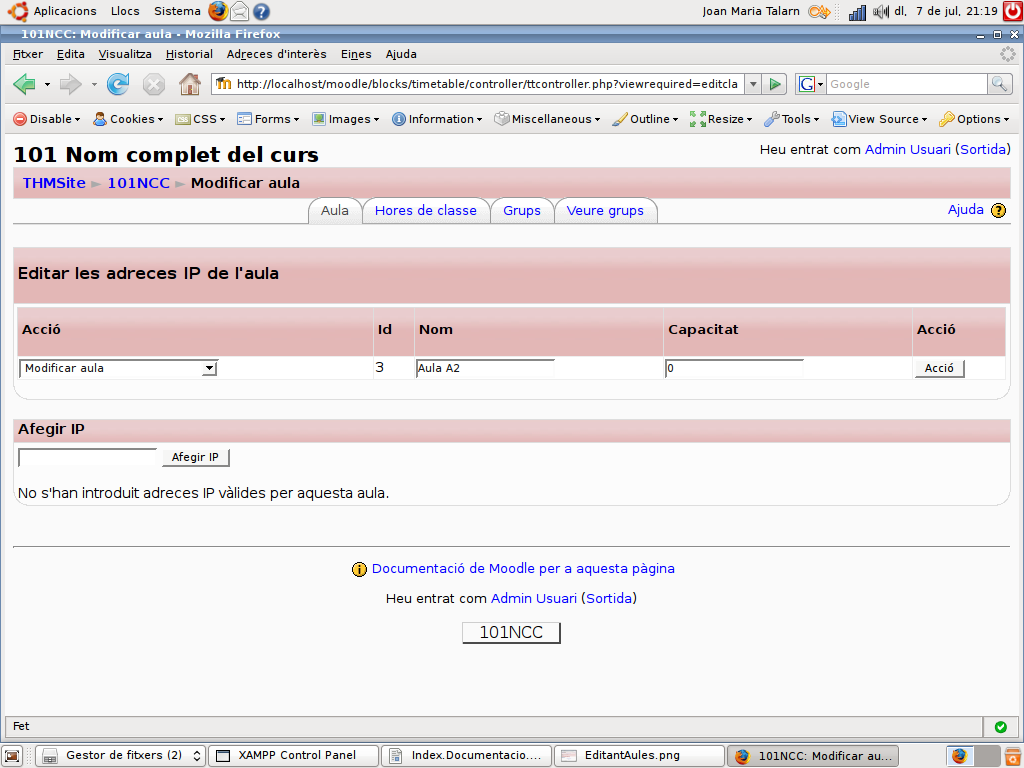
\includegraphics[height=10cm,width=12cm]{img/EditantAdrecesIP.png}
		\caption[List caption]{Pantalla per gestionar adreces IP vàlides per una aula.}
		\label{fig:EditantAdrecesIP}
		\end{center}
		\end{figure}
A la primera secció es poden prendre les mateixes accions que a la secció d'edició de aules però nomès per l'aula se\l.leccionada. A la segona secció és mostrada una llista de les adreces IP afegides (Si no s'han afegit adreces IP es mostrarà un text indicant-ho, com es pot veure a la Figura ~\ref{fig:IPNovalida}) i serà capaç d'afegir una IP al rang o esborrar-la. 
	\begin{itemize}
	\item\textbf{Afegir una IP} - una adreça IP pot ser afegida desde la primera secció d'aquesta segona secció, escrivint-la i prement el botó per Afegir IP. Si la IP no té un format correcte es mostrarà un missatge, tal i com mostra la següent imatge (Figura ~\ref{fig:IPNovalida}).
		\begin{figure}[H] %Here overriding the specifications of Latex good placement
		\begin{center}
		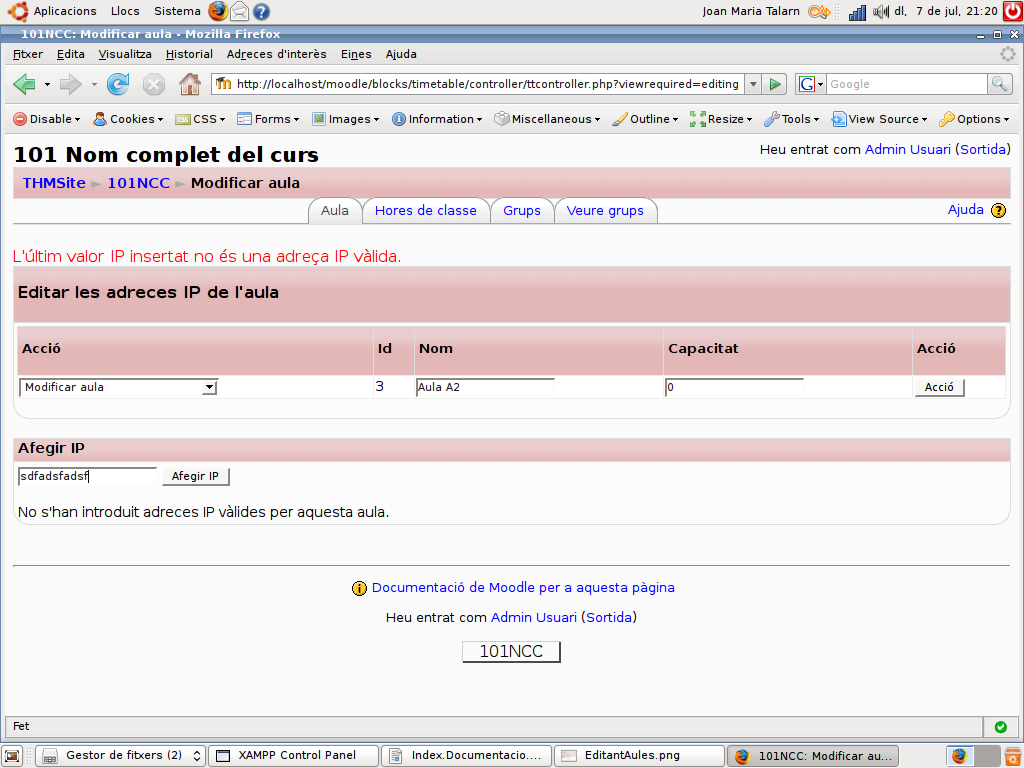
\includegraphics[height=10cm,width=12cm]{img/IPNovalida.png}
		\caption[List caption]{Missatge quan no s'han introduït adreces IP vàlides. El format per l'adreça IP ha de ser correcte.}
		\label{fig:IPNovalida}
		\end{center}
		\end{figure}
	\item\textbf{Esborrar una IP} - a sota de la secció reservada per afegir una IP es mostrat el rang d'adreces IP. Es pot esborrar cadascúna d'aquestes prement el botó per esborrar IP.
	\end{itemize}
\end{itemize}

\section{Editant hores de classe}
Des d'aquesta pàgina (Figura ~\ref{fig:Hourtable}) pot afegir i eliminar les hores de classe que aquesta institució està oferint.
		\begin{figure}[H] %Here overriding the specifications of Latex good placement
		\begin{center}
		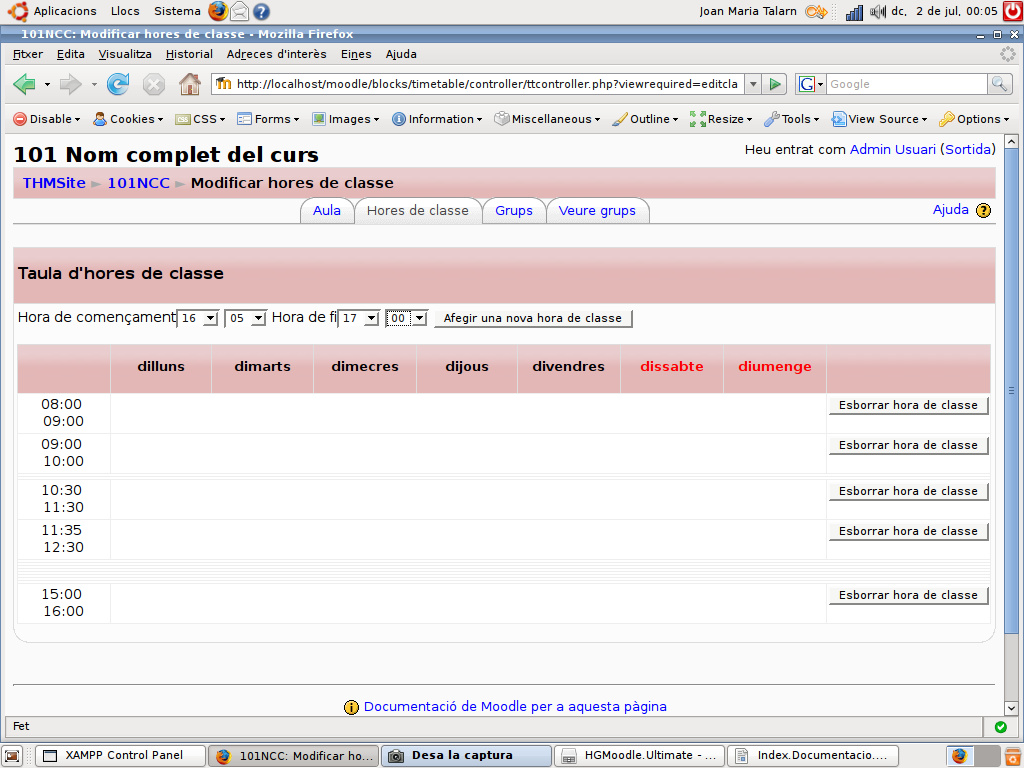
\includegraphics[height=10cm,width=12cm]{img/Hourtable.png}
		\caption[List caption]{Definició d'hores lectives.}
		\label{fig:Hourtable}
		\end{center}
		\end{figure}
\begin{itemize}
\item\textbf{Afegir una hora de classe} - des d'aquesta secció es pot afegir una nova hora de classe.
Ha d'introduir hora d'inici i hora final i clicar el botó Afegir una nova hora de classe i aquesta hora s'afegirà a la llista de baix.
Hora final ha de ser major que hora d'inici, sinó es mostrarà un missatge d'error a la part superior de les seccions tal i com mostra la següent imatge (Figura ~\ref{fig:HourtableError}).
		\begin{figure}[H] %Here overriding the specifications of Latex good placement
		\begin{center}
		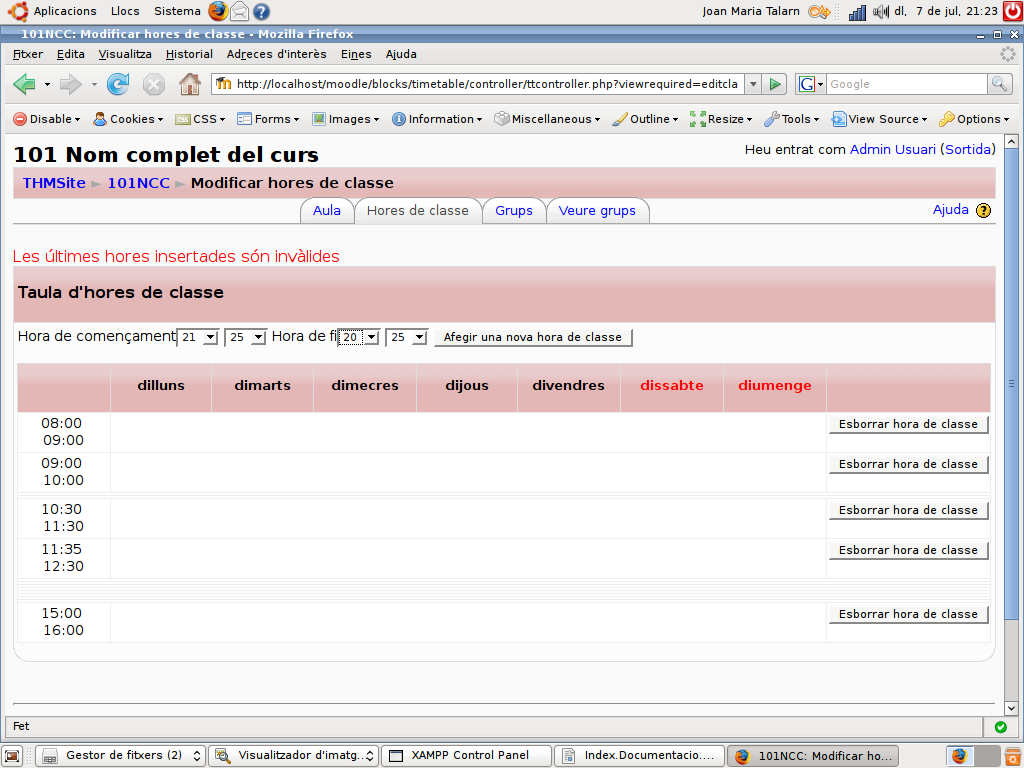
\includegraphics[height=10cm,width=12cm]{img/HourtableError.png}
		\caption[List caption]{Missatge d'error en cas que les hores introduides no siguin correctes.}
		\label{fig:HourtableError}
		\end{center}
		\end{figure}
Per espais de temps de vint minuts entre hores es mostrarà una línia blanca.
\item\textbf{Eliminar hora de classe} - A la part inferior de la secció per a afegir una hora de classe trobarà una llista ordenada de les hores de classe afegides, sinó es mostrarà un missatge que indicarà que no s'han afegit hores de classe.
Per cada fila hi ha un botó d'esborrar. Se li demanarà que confirmi l'acció d'esborrar mitjançant la següent pantalla (Figura ~\ref{fig:HourtableConfirm}):
		\begin{figure}[H] %Here overriding the specifications of Latex good placement
		\begin{center}
		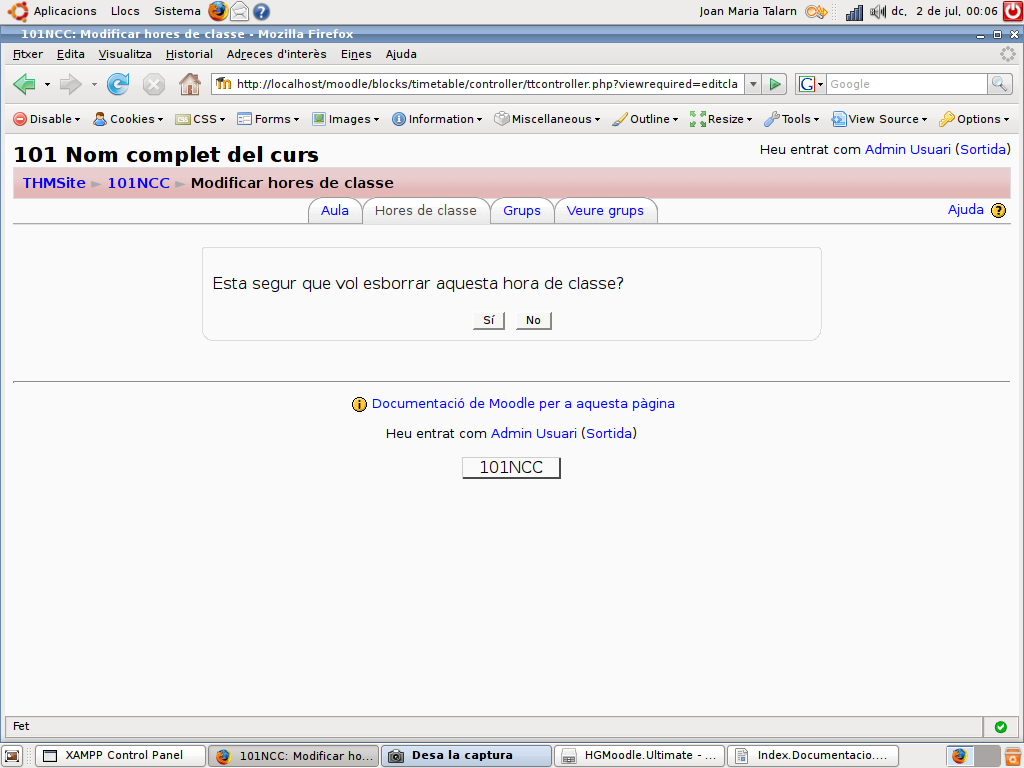
\includegraphics[height=10cm,width=12cm]{img/HourtableConfirm.png}
		\caption[List caption]{Petició de confirmació per esborrar una hora lectiva.}
		\label{fig:HourtableConfirm}
		\end{center}
		\end{figure}
\end{itemize}

\section{Editant Grups}
Des d'aquesta pàgina (Figura ~\ref{fig:EditantGrups}) es pot afegir, modificar i eliminar els grups i els seus horaris per cada curs d'aquesta institució.
		\begin{figure}[H] %Here overriding the specifications of Latex good placement
		\begin{center}
		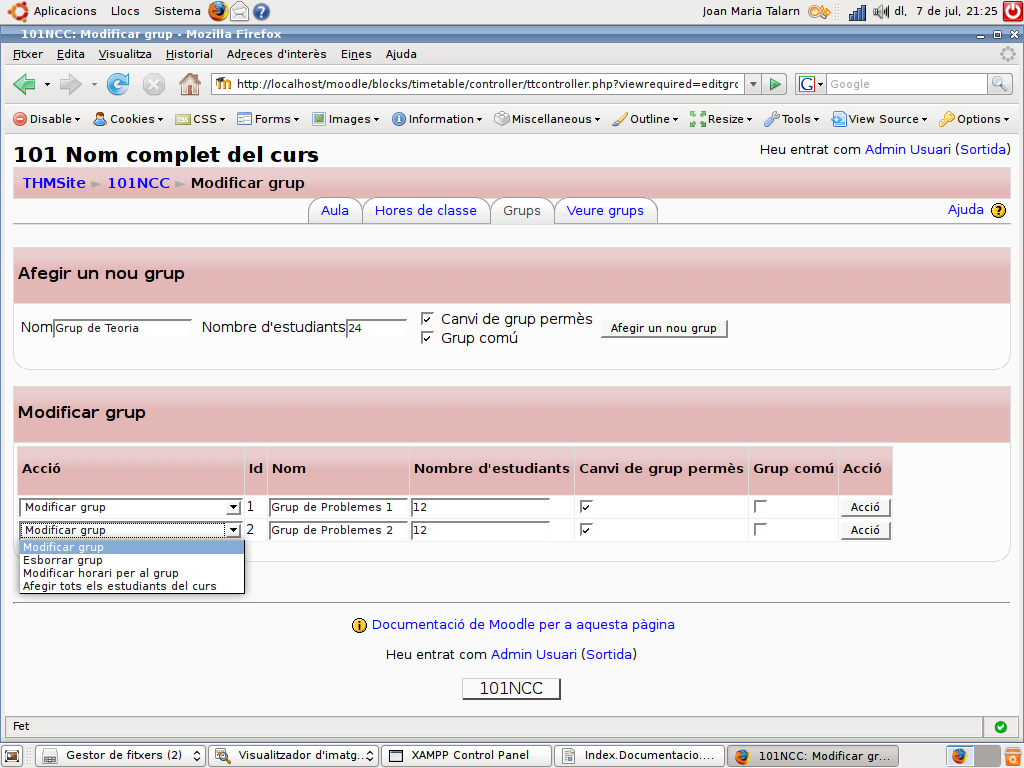
\includegraphics[height=10cm,width=12cm]{img/EditantGrups.png}
		\caption[List caption]{Pantalla per la gestió dels grups.}
		\label{fig:EditantGrups}
		\end{center}
		\end{figure}
\begin{itemize}
\item\textbf{Afegir un grup} - des d'aquesta secció pot afegir un nou grup apretant el botó Afegir un nou grup .
Els paràmetres necessaris per definir un grup són:
	\begin{itemize}
	\item\textbf{nom} - el nom s'utilitza per identificar un grup d'entre els altres grups.
	\item\textbf{número d'alumnes} - el número màxim d'alumnes permesos per apuntar-se al grup. Si s'omet aquest valor s'acaba creant el grup amb 0 places (Figura ~\ref{fig:EditantGrup0places}).
		\begin{figure}[H] %Here overriding the specifications of Latex good placement
		\begin{center}
		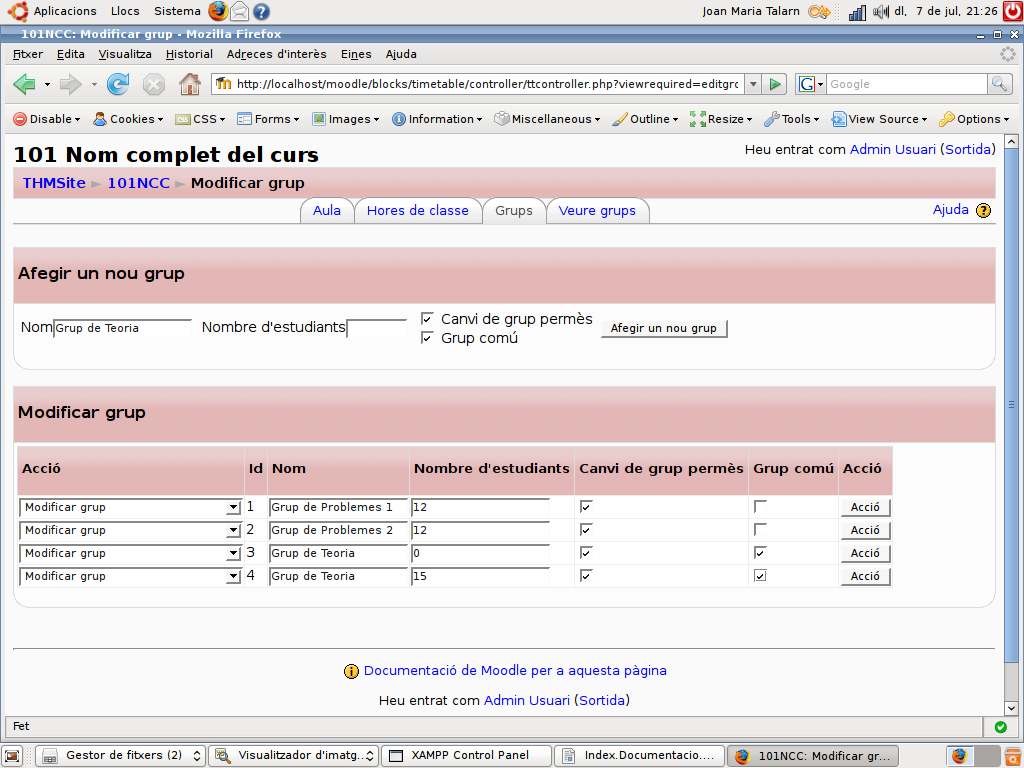
\includegraphics[height=10cm,width=12cm]{img/EditantGrup0places.png}
		\caption[List caption]{Ometent el paràmetre de número d'alumnes es crearà el grup amb 0 places.}
		\label{fig:EditantGrup0places}
		\end{center}
		\end{figure}
	\item\textbf{canvi de grup permès} - el professor pot decidir si un alumne pot esborrar-se del grup ell mateix o ha de ser el professor qui l'esborri del grup.
	\item\textbf{grup comú} – si un grup és comú, això permet poder-se apuntar a aquest grup mentres l'alumne pot ésser apuntat en algún altre.
	Per un grup no comú un usuari només pot apuntar-se en un d'ells, i si l'usuari escull apuntar-se a un altre grup serà esborrat del primer grup.
	\end{itemize}
	
\item\textbf{Editar grup} - des d'aquesta secció pot modificar o eliminar un grup que ja existeix.
Aquesta és una llista de tots els grups disponibles. Si no hi ha grups disponibles un missatge serà mostrat indicant-ho (Figura ~\ref{fig:EditantGrup}).
		\begin{figure}[H] %Here overriding the specifications of Latex good placement
		\begin{center}
		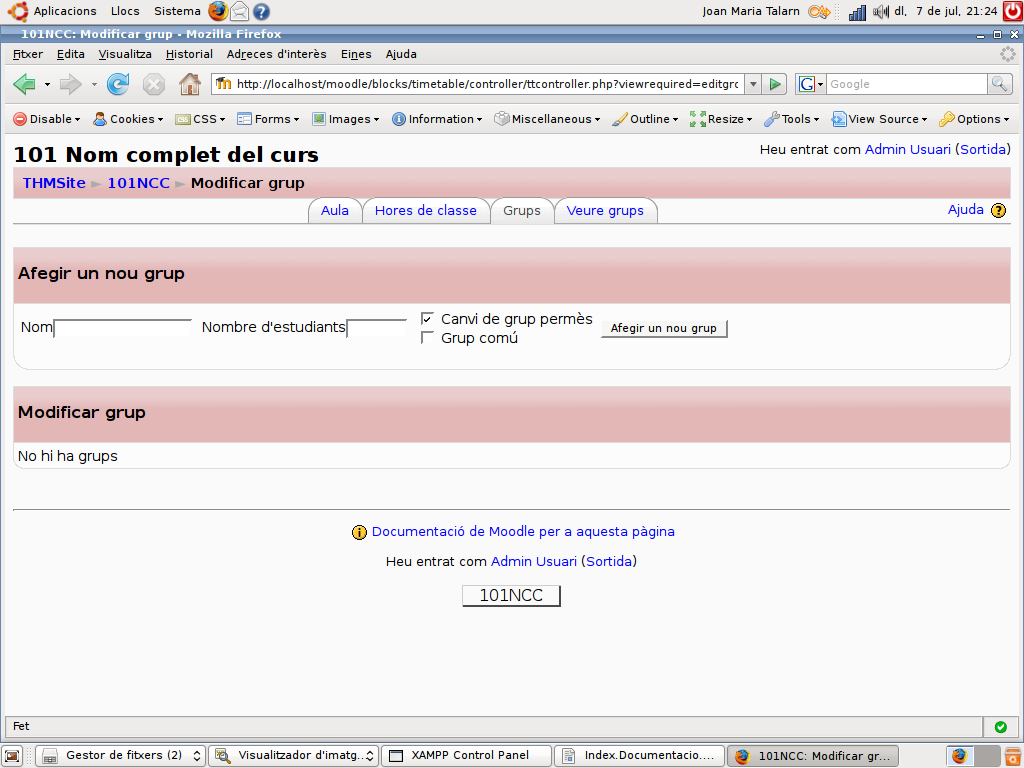
\includegraphics[height=10cm,width=12cm]{img/EditantGrup.png}
		\caption[List caption]{Pantalla per la gestió dels grups.}
		\label{fig:EditantGrup}
		\end{center}
		\end{figure}
Es poden pendre quatre tipus d'accions canviant el valor de la combo d'acció:
	\begin{itemize}
	\item\textbf{Actualitzar grup} - Els paràmetres nom, el número d'alumnes, canvi de grup permès i grup comú es poden modificar per cada fila de la llista però només poden ser actualitzats si aquesta acció és seleccionada a la combo d'acció i el botó d'acció és apretat.
	\item\textbf{Eliminar grup} - el grup pot ser eliminat si aquesta acció és seleccionada i el botó d'acció apretat. Un missatge li demanarà que confirmi l'acció (Figura ~\ref{fig:ConfirmDeleteGrup}).
		\begin{figure}[H] %Here overriding the specifications of Latex good placement
		\begin{center}
		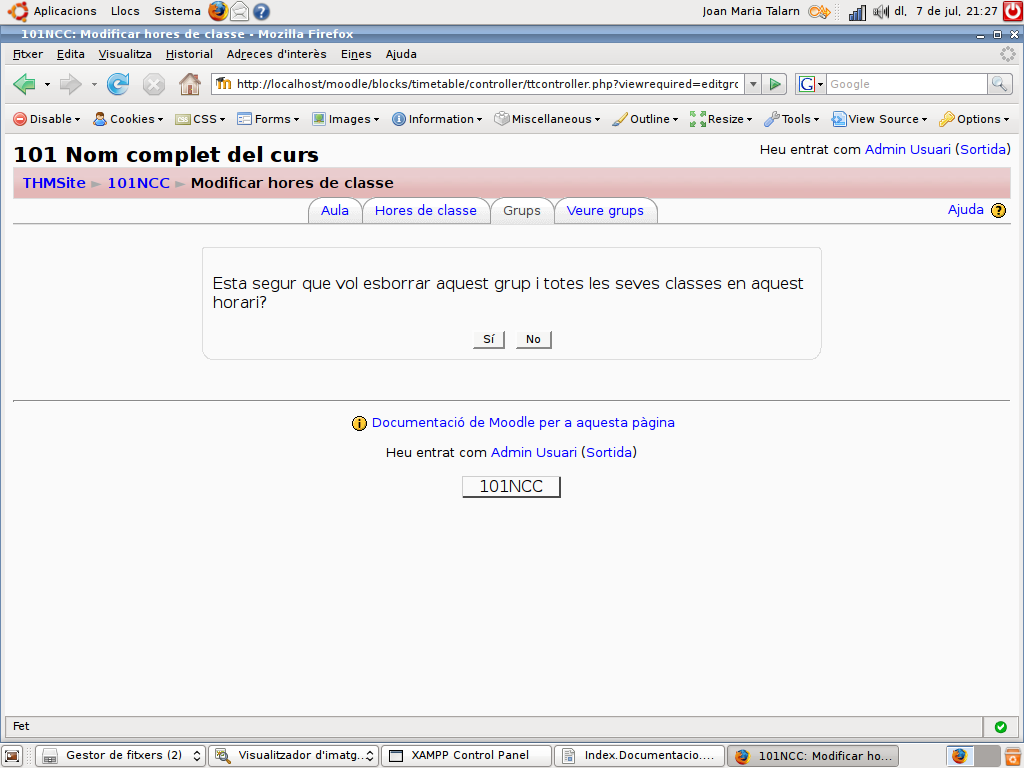
\includegraphics[height=10cm,width=12cm]{img/ConfirmDeleteGrup.png}
		\caption[List caption]{Confirmació per esborrar un grup.}
		\label{fig:ConfirmDeleteGrup}
		\end{center}
		\end{figure}
	\item\textbf{Afegir tots els estudiants del curs} - tots els alumnes del curs seran introduits a la llista un cop el botó d'acció sigui pressionat. Un missatge li demanarà que confirmi l'acció (Figura ~\ref{fig:EditantGrupConfirmAllStudentsIn}).
		\begin{figure}[H] %Here overriding the specifications of Latex good placement
		\begin{center}
		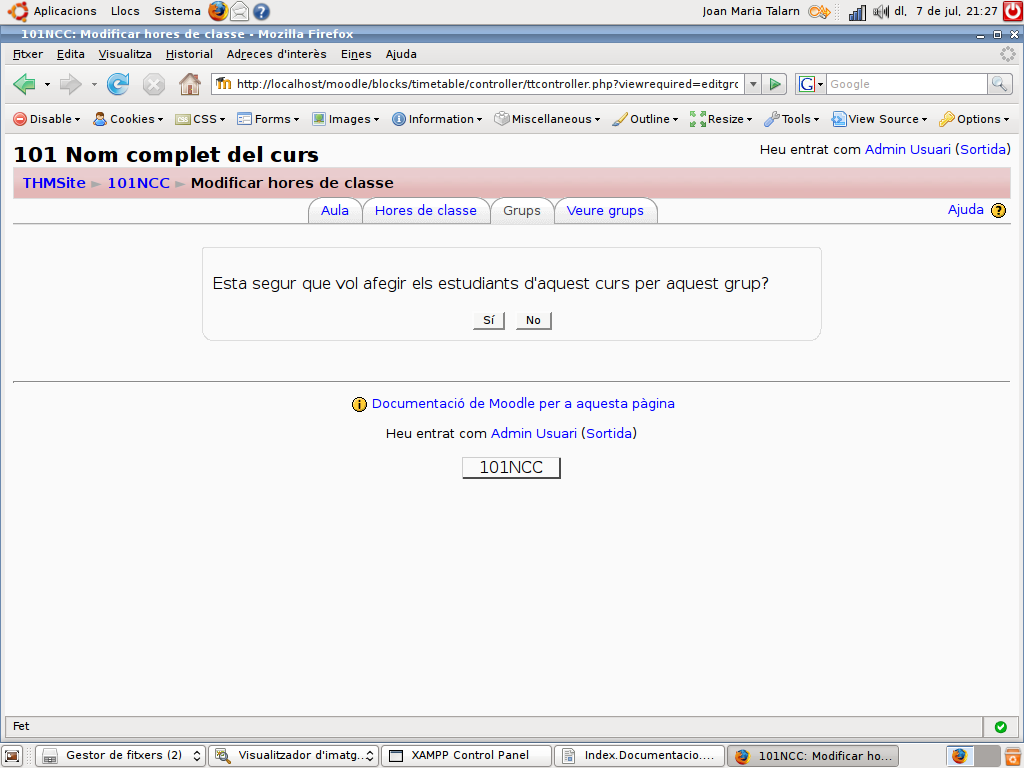
\includegraphics[height=10cm,width=12cm]{img/EditantGrupConfirmAllStudentsIn.png}
		\caption[List caption]{Confirmació per la incorporació de tots els alumnes del curs en aquest grup.}
		\label{fig:EditantGrupConfirmAllStudentsIn}
		\end{center}
		\end{figure}
	\item\textbf{Editar una taula d'hores del grup} - aquesta acció et porta a la pantalla d'edició de l'horari del grup.
	\end{itemize}
	
\item\textbf{Editar una taula d'hores del grup} - des d'aquesta secció (Figura ~\ref{fig:EditantHoresdelgrup}) pot modificar l'horari del grup seleccionat.
		\begin{figure}[H] %Here overriding the specifications of Latex good placement
		\begin{center}
		\includegraphics[height=10cm,width=12cm]{img/EditantHoresdelgrup.png}
		\caption[List caption]{Pantalla per a crear l'horari per cadascún dels grups.}
		\label{fig:EditantHoresdelgrup}
		\end{center}
		\end{figure}
A la primera secció pot fer les mateixes accions que a la secció d'Edició de grup però només pel grup seleccionat. A la segona secció hi ha una representació de la setmana ( dies de cap de setmana< en text vermell) és mostrat amb totes les hores que la institució està donant classes. Per cadascuna d'aquestes caselles es poden fer una d'aquestes dues accions:
	\begin{itemize}
	\item\textbf{Afegir} - Si aquesta acció és possible es motra una combo amb les aules disponibles a la institució per aquesta hora.
	Una classe pot ser afegida seleccionant l'aula apropiada i clicant l'icona afegir.
	Si la capacitat de l'aula és menor que el número d'alumnes que teniem previst un missatge d'alerta en color blau apareixerà a la secció superior i la classe serà afegida en text blau (Figura ~\ref{fig:ModificantHoresGrupAulaPetita}).
		\begin{figure}[H] %Here overriding the specifications of Latex good placement
		\begin{center}
		\includegraphics[height=10cm,width=12cm]{img/ModificantHoresGrupAulaPetita.png}
		\caption[List caption]{Missatge si l'aula té una capacitat menor que el nombre d'alumnes del grup assignat.}
		\label{fig:ModificantHoresGrupAulaPetita}
		\end{center}
		\end{figure}
	Si la classe és afegida en un dia considerat cap de setmana un missatge d'alerta en color blau apareixerà a la secció superior i la classe serà afegida en text blau (Figura ~\ref{fig:EditantHoresdeGrupCapdesetmana}).
		\begin{figure}[H] %Here overriding the specifications of Latex good placement
		\begin{center}
		\includegraphics[height=10cm,width=12cm]{img/EditantHoresdeGrupCapdesetmana.png}
		\caption[List caption]{Missatge si la classe és assignada en un dia considerat no lectiu pel centre.}
		\label{fig:EditantHoresdeGrupCapdesetmana}
		\end{center}
		\end{figure}
	Si passen tots dos casos alhora es mostren tots dos missatges alhora (Figura ~\ref{fig:ModifcarHoresGrupTotesduesadvertencies}).
		\begin{figure}[H] %Here overriding the specifications of Latex good placement
		\begin{center}
		\includegraphics[height=10cm,width=12cm]{img/ModifcarHoresGrupTotesduesadvertencies.png}
		\caption[List caption]{Missatge amb les dues advertències alhora.}
		\label{fig:ModifcarHoresGrupTotesduesadvertencies}
		\end{center}
		\end{figure}
	\item\textbf{Eliminar} - Si una classe va ser afegida la pot eliminar clicant la icona Eliminar.
	\end{itemize}
	
\end{itemize}

\section{Veient els grups}
Des d'aquesta pàgina (Figura ~\ref{fig:VeureGrup}) pot veure els alumnes apuntats al grup i l'horari del grup seleccionat.
		\begin{figure}[H] %Here overriding the specifications of Latex good placement
		\begin{center}
		\includegraphics[height=10cm,width=12cm]{img/VeureGrup.png}
		\caption[List caption]{Pantalla per a la visualització d'informació dels grups vista amb el rol d'administrador.}
		\label{fig:VeureGrup}
		\end{center}
		\end{figure}
Depenent del rol de l'usuari es veuen unes o altres accions a realitzar (Figura ~\ref{fig:VeureGrupRolStudent}):
		\begin{figure}[H] %Here overriding the specifications of Latex good placement
		\begin{center}
		\includegraphics[height=10cm,width=12cm]{img/VeureGrupRolStudent.png}
		\caption[List caption]{Pantalla per a la visualització d'informació dels grups vista amb el rol d'estudiant.}
		\label{fig:VeureGrupRolStudent}
		\end{center}
		\end{figure}
\begin{itemize}
\item\textbf{Veure el grup d'alumnes} - seleccionant un grup al combo i l'acció veure alumnes del grup veurà una llista de tots els alumnes apuntats (Figura ~\ref{fig:VeureGrupEstudiantsRolStudent}) sinó un missatge indicarà que no s'hi han apuntat alumnes (Figura ~\ref{fig:VeureGrupEstudiantsNingu}).
		\begin{figure}[H] %Here overriding the specifications of Latex good placement
		\begin{center}
		\includegraphics[height=10cm,width=12cm]{img/VeureGrupEstudiantsRolStudent.png}
		\caption[List caption]{Llistat dels alumnes apuntats al grup vist amb el rol d'estudiant.}
		\label{fig:VeureGrupEstudiantsRolStudent}
		\end{center}
		\end{figure}

		\begin{figure}[H] %Here overriding the specifications of Latex good placement
		\begin{center}
		\includegraphics[height=10cm,width=12cm]{img/VeureGrupEstudiantsNingu.png}
		\caption[List caption]{Missatge si no hi han alumnes apuntats al grup.}
		\label{fig:VeureGrupEstudiantsNingu}
		\end{center}
		\end{figure}

Si té permisos pot excloure l'alumne del grup (Figura ~\ref{fig:VeureGrupEstudiantsTotsalli}).
		\begin{figure}[H] %Here overriding the specifications of Latex good placement
		\begin{center}
		\includegraphics[height=10cm,width=12cm]{img/VeureGrupEstudiantsTotsalli.png}
		\caption[List caption]{Llistat dels alumnes apuntats al grup vist amb el rol d'administrador.}
		\label{fig:VeureGrupEstudiantsTotsalli}
		\end{center}
		\end{figure}

		\begin{figure}[H] %Here overriding the specifications of Latex good placement
		\begin{center}
		\includegraphics[height=10cm,width=12cm]{img/VeureGrupEsborrantUsuari.png}
		\caption[List caption]{Confirmació a l'hora de treure un alumne d'un grup.}
		\label{fig:VeureGrupEsborrantUsuari}
		\end{center}
		\end{figure}
		
\item\textbf{Veure la taula d'hores del grup} - seleccionant un grup al combo i l'acció veure la taula d'hores del grup veurà un horari pel grup seleccionat (Figura ~\ref{fig:VeureGrupsHorari}).
		\begin{figure}[H] %Here overriding the specifications of Latex good placement
		\begin{center}
		\includegraphics[height=10cm,width=12cm]{img/VeureGrupsHorari.png}
		\caption[List caption]{Visualització del horari pel grup amb l'opció d'apuntar-shi (Botó a la part superior dreta).}
		\label{fig:VeureGrupsHorari}
		\end{center}
		\end{figure}
Vostè es pot apuntar al grup seleccionat pulsant el botó a la part superior dreta del horari.
		\begin{figure}[H] %Here overriding the specifications of Latex good placement
		\begin{center}
		\includegraphics[height=10cm,width=12cm]{img/VeureGrupConfirmaApuntarse.png}
		\caption[List caption]{Confirmació a l'hora d'apuntar-se a un grup.}
		\label{fig:VeureGrupConfirmaApuntarse}
		\end{center}
		\end{figure}

Si ja s'ha apuntat al grup apareixerà un missatge indicant-ho al lloc del botó (Figura ~\ref{fig:VeureGrupJaMeapuntat}).
		\begin{figure}[H] %Here overriding the specifications of Latex good placement
		\begin{center}
		\includegraphics[height=10cm,width=12cm]{img/VeureGrupJaMeapuntat.png}
		\caption[List caption]{Visualització del horari pel grup al qual ja s'ha apuntat.}
		\label{fig:VeureGrupJaMeapuntat}
		\end{center}
		\end{figure}

\item\textbf{Veure l'assistència del grup} - seleccionant un grup a la combo i l'acció veure l'assistència del grup es veurà l'assistència dels estudiants apuntats al grup i la seva IP per cada cop que l'estudiant s'hagi connectat durant l'última setmana al lloc Moodle (Figura ~\ref{fig:VeureGrupsLogAssistenciaIPNoValidaIpValida}).
		\begin{figure}[H] %Here overriding the specifications of Latex good placement
		\begin{center}
		\includegraphics[height=10cm,width=12cm]{img/VeureGrupsLogAssistenciaIPNoValidaIpValida.png}
		\caption[List caption]{Visualització del horari pel grup al qual ja s'ha apuntat.}
		\label{fig:VeureGrupsLogAssistenciaIPNoValidaIpValida}
		\end{center}
		\end{figure}
Els professors poden canviar el rang de dates amb les combos de la part superior d'aquesta secció. 
Per cada classe per aquest grup es mostra la data,l'hora i el nom de la classe(l'id en cas d'omisió) i la llista d'estudiants en una vista de matriu.
Un missatge definit es mostrarà si no hi ha hagut connexió al lloc Moodle, la IP en vermell per una IP de connexió no vàlida al moment de la classe mostrada a la capçalera, i la IP en negre per una connexió correcta (assumint per connexió correcta una IP dins el rang de IPs vàlides per l'aula a l'hora que es va fer aquella  classe).
Si el interval no es correcte es mostrarà un missatge indicant-ho. Sino hi han hagut classes durant el període seleccionat es mostra un missatge indicant-ho (Figura ~\ref{fig:VeureGrupDatesNoValides}).
		\begin{figure}[H] %Here overriding the specifications of Latex good placement
		\begin{center}
		\includegraphics[height=10cm,width=12cm]{img/VeureGrupDatesNoValides.png}
		\caption[List caption]{Missatge d'error si el rang és invàlid (en vermell a la part superior) i missatge si entre les dates escollides no hi han hagut registres.}
		\label{fig:VeureGrupDatesNoValides}
		\end{center}
		\end{figure}
\end{itemize}

\chapter{Avaluacions} 
Durant el període de desenvolupament s'ha pogut comprovar que el bloc té un funcionament correcte sobre moltes plataformes i navegadors web. A continuació és detalla quins han estat aquests escenaris de proves, tant la part on ha estat insta\l.lat el servidor Moodle com en quins navegadors s'ha provat.
\section{Servidor}
Aquest bloc de Moodle es va començar a desenvolupar en un servidor local XAMPP sobre Windows XP.\\
\begin{quote}
XAMPP és un paquet de programari lliure que conté el servidor HTTP Apache, base de dades de MySQL i eines necessàries per utilitzar el PHP i el llenguatge de programació Perl. El programa es llança sota el GNU de Llicència Pública General i d'un servidor web, d'ús fàcil, capaç de servir pàgines dinàmiques. Actualment, XAMPP està disponible per a Windows, Linux, Solaris i Mac OS X (el X en el seu nom podria estar dret per a un qualsevol d'aquests sistemes operatius.
\end{quote}
XAMPP és pot obtenir d'aquesta url \url{http://www.apachefriends.org/en/xampp.html}.\\

Es van començar les proves i el desenvolupament amb la versió 1.7 de Moodle, i més tard tal com indica el capitol sobre la versió de Moodle necessària (Secció \ref{VersioMoodle}, pàgina \pageref{VersioMoodle} ) amb la versió 1.8, concretament amb la versió 1.8.7.\\
Localment s'ha provat, posteriorment, aquest bloc amb una versió de XAMPP corrent sobre Linux Ubuntu (Primer amb la versió 7.10 i després sobre la versió 8.4). Aquest servidor XAMPP és composat per:
\begin{itemize}
	\item Servidor Web Apache 2.2.8
	\item Servidor de Base de dades MySQL 5.0.51a
	\item PHP Versió 5.2.5 
\end{itemize}

Per continuar amb les proves i el desenvolupament es va passar a insta\l.lar, també primer la versió de Moodle 1.7 i posteriorment la 1.8 (Moodle 1.8.3 primer i Moodle 1.8.7 després) en un servidor de hosting gratuït amb les següents especificacions.
\begin{itemize}
	\item Sistema Operatiu Linux
	\item Servidor Web Apache Versió 2.2.10 (Unix)
	\item PHP Versió 5.2.6
	\item Servidor de Base de dades MySQL Version 5.0.51
\end{itemize}
Va ser en aquest servidor de hosting gratuït, situat a Nova York on es va descobrir el problema de la versió mínima (Secció \ref{DesenvolupamentFuncioTime}, pàgina \pageref{DesenvolupamentFuncioTime}). Aquest servidor es pot trobar a \url{http://jmtalarn.byethost10.com/moodle}.
\section{Client}
Per confirmar el correcte funcionament en el màxim nombre de clients, s'ha comprovat un funcionament correcte amb el següent llistat de navegadors web:
\begin{itemize}
	\item Internet Explorer 6 amb Windows XP
	\item Internet Explorer 7 amb Windows XP
	\item Firefox 2 amb Windows XP
	\item Firefox 3 amb Windows XP
	\item Safari amb Windows XP 
	\item Firefox 2 amb Ubuntu 7.10
	\item Firefox 2 amb Ubuntu 8.4
	\item Firefox 3 amb Ubuntu 8.4
	\item Konqueror amb Ubuntu 8.4 
\end{itemize}


\chapter{Conclusions}
Moodle és una servidor de continguts per a centres educatius, on, vist la experiència i sobre molts comentaris que es poden trobar als forums de Moodle, el seu èxit es deu principalment sobre la possibilitat d'instalar-ho en multiples plataformes sense masses complicacions.\\ 
Tanmateix, aquest projecte ha servit per comprovar que la principal avantatge del software lliure no recau en la seva gratuïtat, tot i que sí que es tracta d'una gran avantatge, sinó en la comunitat que l'envolta.\\
La comunitat Moodle, com moltes altres comunitats de software lliure, és una comunitat amb moltissima activitat i una gran quantitat de recursos disponibles per a consultar sobre qualsevol dels àmbits (insta\l.lació, desenvolupament, ús, etc.) que pot implicar l'implementació d'una so\l.lució Moodle mitjançant els fòrums, documents i seguiment d'incidències. \\
Tota aquesta informació està total o parcialment traduïda a moltissimes llengües, fet que també repercuteix en la seva amplia difusió ja que el fa accessible a molta gent.\\
És en aquesta comunitat d'on s'ha extret gairebé tot el suport per al desenvolupament d'aquest projecte.\\
Aquest desenvolupament ha servit principalment en veure quina pot ser la complexitat en el desenvolupament de les unitats de software. I com tota planificació de qualsevol projecte, encara que sigui molt importat i d'obligatorietat, pot ser afectada i modificada per múltiples factors i acabant desviant la previsió inicial; recursivament, una bona previsió serveix per preveure aquestes situacions o si més no, de quina manera poden ser corregides. 

\chapter{Annex. Extractes de la documentació utilitzada.}
En aquest capítol s'inclouen extractes de la documentació utilitzada per l'elaboració d'aquest bloc de Moodle. En aquest document es troben referències a aquest capítol per clarificar aquells punts on podria ser necessària una lectura del material utilitzat per la presa de decisions o resolució de problemes.
\section{Definint el fitxer xmldb}\label{annexxmldb}
\begin{otherlanguage}{english}
\begin{quote}

\begin{minipage}{10cm}
{\bfseries Development:XMLDB defining an XML structure}
\end{minipage}
\hfill
\begin{minipage}{2.51cm}
		\begin{figure}[H] %Here overriding the specifications of Latex good placement
		\begin{center}
		\includegraphics[width=2.51cm]{img/Moodle17.png}
		\label{fig:Moodle17}
		\end{center}
		\end{figure}

\end{minipage}
\\
{\bfseries Justification}\\
Before Moodle 1.7, all the DB install and upgrade was developed twice (once to handle MySQL installations and another to handle PostgreSQL installations). This approach, although working, has caused some headaches in the past, mainly because it was really difficult to keep both lines of development 100\% on sync.\\
Some developers do they work against one RDBMS and it was complex to develop to the other one (two test environments, skills on both databases, slower development cycle...). And all this was happening with only two supported RDBMS!\\
One of the main objectives of Moodle 1.7 is to extend the the number of supported RDBMS to other flavours (more exactly, to Oracle and MSSQL). And the old approach (one line of development for each DB) could become an absolute nightmare.\\
Because of this we have planned to build one structure to define all the DB objects used by Moodle. This structure will provide the necessary level of abstraction to be shared by all the RDBMS systems, so the $"$multiple lines of development$"$ explained in the previous paragraph will be out forever, giving us one robust and well defined way to handle DB objects independently of the exact RDBMS being used.\\
{\bfseries Implementation}\\
Initially all our best wishes were to use the AdoDB XML Schema (\url{http://phplens.com/lens/adodb/docsdatadict.htm\#xmlschema}).\\
As Moodle is using ADOdb libraries to communicate with databases it sounded like the natural approach to solve the problem. But, finally, two reasons prevented us to use it:
\begin{enumerate}
\item Although working, it seems to be one feature in progress, with important changes/evolutions arriving at the time of write this document.
\item Its lack of support for $"$prefixes$"$ (one Moodle key feature, to allow multiple instances to run in the same server), would force us to create some awful tricks to generate the objects.
\end{enumerate}
So, finally, we decided to build our own XML files, with everything we need to define every object present in the DB.\\
{\bfseries The XMLDB editor}\\
Although the XML is pretty simple to read (and to write), one of the major drawbacks was its easy and errorprone adoption by the developers. Also some problems with versioning systems getting crazy with XML files (thanks ML!) pointed us to the requirement to use one high-density format (it means, physically long lines) in our XML files.\\
After some intense thoughts we decided to build one specialised editor for our XML format. This editor should be easy to use and provide support for all the objects present one Moodle DB. And it's done (and will support future enhancements easily, we hope).\\
The XMLDB Editor makes the edition of tables/fields/keys/indexes practically a trivial task, allowing the developer to spend the time coding and improving things instead of fighting against XML files and the errors caused by manual editing (of course, the developer is free to use such extra-time as desired, beers, dance,books, music...) ;-)\\
All the new install.xml files, present under each db directory in Moodle can be edited (and we recommend it) with just some clicks and keystrokes. Those install.xml will contain all the info needed to generate the specific objects needed for each RDBMS supported. Obviously, such files, are the neutral replacement for all the *.sql files used until now.\\
{\bfseries Launching}\\
Just login to your server as an administrator and, under the Miscellaneous tab of the Administration Block, you'll see a new link pointing to the $"$XMLDB Editor$"$.\\
One important note is that, to be able to handle files properly, the web server needs write access to all those $"$db$"$ directories where the $"$install.xml$"$ files reside (and to the files themselves, of course). ;-)\\
That's all!\\
{\bfseries Use}\\
We really think the XMLDB Editor is pretty easy to use, so here you won't see a complete guide to use it. We highly recommend you to play with it for a while, viewing how it works and how it modifies the install.xml files.\\
It's organised in a top-botton structure, where you start loading (or creating) a new XMLDB file. Then, you can edit such file and its general structure will be showed. This structure have two type of elements, tables and statements and the XMLDB Editor allows you to add, edit, delete, and move them easily. Also, for initial creation of tables, one small but effective reverse-enginery tool has been developed (only under MySQL) allowing you to retrofit any table from the DB to the XMLDB Editor.\\
While editing tables you will see their fields, keys and indexes and you'll be able to handle all them easily.\\
Note that some fields can be no-editable. It uses to be because they are being used in some way (part of one key or index) and the idea is to warn you about that.\\
Fields can be edited and you can specify their name, type, length, decimals, null-ability, defaults and so one. Exactly the same for both keys and indexes.\\
While editing statements, you must think about them like $"$collections of sentences$"$. Once you select the type (only inserts are allowed for now) and table you are interested you'll be able to introduce the exact values easily, being able to duplicate them easily to gain some speed if you have a lot of sentences in your development. Sentences can be edited and deleted easily too.\\
One interesting feature is that all the XMLDB Editor pages allow you to enter one comment about the item being modified (table, index, key, field, statement...). Use it at your entire needs, sure it helps other developers to understand a bit more the DB model.\\
Please, don't forget to read and understand the next section, where we talk about some important guidelines to create and handle XMLDB files.\\
\end{quote}
\end{otherlanguage}

\section{Variables globals}\label{annexvariablesglobals}
\begin{otherlanguage}{spanish}
\begin{quote}
Moodle maneja la información más recurrida mediante variables globales a las cuales tiene acceso desde todos los ficheros que desee (si no conoces mucho sobre PHP, te sugiero que busques información sobre el tema en webs como \url{www.lawebdelprogramador.com} o \url{www.webalia.com}). Estas variables globales son las siguientes:\\
\$CFG: Es relativo a la configuración del curso, guarda los valores sobre la dirección raíz del sistema (wwwroot) o el prefijo de las tablas de la BDD (prefix) entre otras cosas.\\ 
\$SESSION: Guarda los datos sobre cada sesión abierta (creo que se refiere a las cookies que crea al iniciar cada una de las sesiones, pero esto deberías confirmarlo).\\
\$THEME: Esta variable se refiere al modelo de interfaz que estas usando, los que se encuentran en el directorio /moodle/theme\\
\$SITE: Sinceramente no recuerdo para que vale.\\
\$COURSE: Esta es muy importante ya que sirve para conecer toda la información sobre los cursos sin necesidad de buscar en cada momento la información del curso actual.\\
\$USER: Igualmente, esta variable contiene toda la información útil sobre cada usuario. Por ejemplo para acceder a su identificador se puede acceder como \$USER->id\\
Con estas variables tendrás casi toda la información que puedas necesitar en un momento dado, pero de todas formas puedes hacer consultas y demás usando las funciones que ya ha implementado Moodle o tus propias consultas.
Moodle además guarda un log de todo lo que ocurre en el sitio mediante una tabla de la base de datos (tabla log como te comenté). Los resultados se muestran por ejemplo cuando se accede a la consulta de registros como administrador. 
Si cuando implementes tus módulos, bloques, o lo que quieras hacer, quieres que se guarde un log, es suficiente con que uses la función que te comentaba en el post anterior (add\_to\_log). No recuerdo muy bien la sintaxis que tiene, pero te sugiero que busques en cualquier archivo de moodle que guarde información en el registro (sobre cursos, accesos al sitio o cualquier otra cosa) y observes su comportamiento, porque es realmente sencillo.
\end{quote} 
\end{otherlanguage}

\section{Definició de rols. Fitxer access.db.}\label{annexrols}
\begin{otherlanguage}{english}
\begin{quote}
\begin{minipage}{10cm}
{\bfseries Programming Interface}
\end{minipage}
\hfill
\begin{minipage}{2.51cm}
		\begin{figure}[H] %Here overriding the specifications of Latex good placement
		\begin{center}
		\includegraphics[width=2.51cm]{img/Moodle17.png}
		\label{fig:Moodle17}
		\end{center}
		\end{figure}

\end{minipage}
\\
Although the Roles system may look complicated at first glance, implementing it in Moodle code is fairly simple. 
You need to define each capability once, so that Moodle can upgrade existing roles to take advantage of it. You do this in an access.php inside the db folder of any module (eg see mod/forum/db/access.php). The array contains entries like this (note the descriptions for the legacy roles which provides forward compatibility): 
\begin{lstlisting}[style=PHP]
   'mod/forum:viewforum' => array(
       'captype' => 'read',
       'contextlevel' => CONTEXT_MODULE,
       'legacy' => array(
           'guest' => CAP_PREVENT,
           'student' => CAP_ALLOW,
           'teacher' => CAP_ALLOW,
           'editingteacher' => CAP_ALLOW,
           'coursecreator' => CAP_ALLOW,
           'admin' => CAP_ALLOW
       )
   ),
\end{lstlisting}
To load/change these capabilities you need to bump the module version. There's no need to provide changes or differences as Moodle will scan the whole array and sort it out. 
On each page you need to find the context the user is working in, using the get\_context\_instance() function. For example, in the forum module: 
\begin{lstlisting}[style=PHP]
 $context = get_context_instance(CONTEXT_MODULE, $cm->id);
\end{lstlisting}
Then, whenever you want to check that the current user has rights to do something, call has\_capability() like this: 
\begin{lstlisting}[style=PHP]
   if (!has_capability('mod/forum:viewforum', $context)) {
       print_error('nopermissiontoviewforum');
   }
\end{lstlisting}
If you just want to assert a capability and then finish with an error message if it's not met (as we did above), then a shorter way it to use require\_capability() like this: 
\begin{lstlisting}[style=PHP]
   require_capability('mod/forum:viewforum', $context);
\end{lstlisting}
Note that there are extra parameters you can specify to get a custom error message, otherwise users get an automated $"$No permissions$"$ message that lists the permission they were missing. 

As a result of the new Roles System, all calls to isadmin(), iscoursecreator(), isteacheredit(), isteacher(), isstudent(), and isguest() will have to be replaced with calls to has\_capability() or require\_capability(). However, these functions will be retained for some backward compatibility with old code, using the legacy capabilities to try and work out what to do. 
\end{quote}
\end{otherlanguage}

\section{Funcions d'accès a dades.}\label{annexaccesdades}
%\begin{lstlisting}[style=PHP, caption=Funcions de manegament d'objectes de l'API de Moodle]
\begin{tt}
\begin{center}
   \begin{tabular}{| p{12cm} |}
	\hline
	\rowcolor[gray]{0.5}get\_record(\$table, \$field1, \$value1, \$field2='', \$value2='', \$field3='', \$value3='', \$fields='*') X-Ref\\
	Get a single record as an object\\
	\hline
	param: string \$table The table to select from.\\
	param: string \$field1 the first field to check (optional).\\
	param: string \$value1 the value field1 must have (requred if field1 is given, else optional).\\
	param: string \$field2 the second field to check (optional).\\
	param: string \$value2 the value field2 must have (requred if field2 is given, else optional).\\
	param: string \$field3 the third field to check (optional).\\
	param: string \$value3 the value field3 must have (requred if field3 is given, else optional).\\
	return: mixed a fieldset object containing the first mathcing record, or false if none found.\\
	\hline
	\end{tabular}
	\     \ \\ \     \ \\
   \begin{tabular}{| p{12cm} |}
	\hline
	\rowcolor[gray]{0.5}get\_record\_sql(\$sql, \$expectmultiple=false, \$nolimit=false) X-Ref\\
	Get a single record as an object using an SQL statement\\
	\hline
	The SQL statement should normally only return one record. In debug mode\\
	you will get a warning if more record is returned (unless you\\
	set \$expectmultiple to true). In non-debug mode, it just returns\\
	the first record.\\
	\\
	param: string \$sql The SQL string you wish to be executed, should normally only return one record.\\
	param: bool \$expectmultiple If the SQL cannot be written to conveniently return just one record,\\
	param: bool \$nolimit sometimes appending ' LIMIT 1' to the SQL causes an error. Set this to true\\
	return: Found record as object. False if not found or error\\
	\hline
	\end{tabular}
	\     \ \\ \     \ \\
   \begin{tabular}{| p{12cm} |} 
	\hline
	\rowcolor[gray]{0.5}get\_record\_select(\$table, \$select='', \$fields='*') X-Ref\\
	Gets one record from a table, as an object\\
	\hline
	param: string \$table The database table to be checked against.\\
	param: string \$select A fragment of SQL to be used in a where clause in the SQL call.\\
	param: string \$fields A comma separated list of fields to be returned from the chosen table.\\
	return: object|false Returns an array of found records (as objects) or false if no records or error occured.\\
	\hline
	\end{tabular}
	\     \ \\ \     \ \\
   \begin{tabular}{| p{12cm} |} 
	\hline
	\rowcolor[gray]{0.5}get\_records(\$table, \$field='', \$value='', \$sort='', \$fields='*', \$limitfrom='', \$limitnum='') X-Ref\\
	Get a number of records as an array of objects.\\
	\hline
	If the query succeeds and returns at least one record, the\\
	return value is an array of objects, one object for each\\
	record found. The array key is the value from the first\\
	column of the result set. The object associated with that key\\
	has a member variable for each column of the results.\\
	\\
	param: string \$table the table to query.\\
	param: string \$field a field to check (optional).\\
	param: string \$value the value the field must have (requred if field1 is given, else optional).\\
	param: string \$sort an order to sort the results in (optional, a valid SQL ORDER BY parameter).\\
	param: string \$fields a comma separated list of fields to return (optional, by default\\
	param: int \$limitfrom return a subset of records, starting at this point (optional, required if \$limitnum is set).\\
	param: int \$limitnum return a subset comprising this many records (optional, required if \$limitfrom is set).\\
	return: mixed an array of objects, or false if no records were found or an error occured.\\
	\hline
	\end{tabular}
	\     \ \\ \     \ \\
   \begin{tabular}{| p{12cm} |} 
	\hline
	\rowcolor[gray]{0.5}get\_records\_select(\$table, \$select='', \$sort='', \$fields='*', \$limitfrom='', \$limitnum='') X-Ref\\
	Get a number of records as an array of objects.\\
	\hline
	Return value as for @see function get\_records.\\
	\\
	param: string \$table the table to query.\\
	param: string \$select A fragment of SQL to be used in a where clause in the SQL call.\\
	param: string \$sort an order to sort the results in (optional, a valid SQL ORDER BY parameter).\\
	param: string \$fields a comma separated list of fields to return\\
	param: int \$limitfrom return a subset of records, starting at this point (optional, required if \$limitnum is set).\\
	param: int \$limitnum return a subset comprising this many records (optional, required if \$limitfrom is set).\\
	return: mixed an array of objects, or false if no records were found or an error occured.\\
	\hline
	\end{tabular}
	\     \ \\ \     \ \\
   \begin{tabular}{| p{12cm} |} 
	\hline
	\rowcolor[gray]{0.5}get\_records\_list(\$table, \$field='', \$values='', \$sort='', \$fields='*', \$limitfrom='', \$limitnum='') X-Ref\\
	Get a number of records as an array of objects.\\
	\hline
	Return value as for @see function get\_records.\\
	\\
	param: string \$table The database table to be checked against.\\
	param: string \$field The field to search\\
	param: string \$values Comma separated list of possible value\\
	param: string \$sort Sort order (as valid SQL sort parameter)\\
	param: string \$fields A comma separated list of fields to be returned from the chosen table. If specified,\\
	return: mixed an array of objects, or false if no records were found or an error occured.\\
	\hline
	\end{tabular}
	\     \ \\ \     \ \\
   \begin{tabular}{| p{12cm} |} 
	\hline
	\rowcolor[gray]{0.5}get\_records\_sql(\$sql, \$limitfrom='', \$limitnum='') X-Ref\\
	Get a number of records as an array of objects.\\
	\hline
	Return value as for @see function get\_records.\\
	\\
	param: string \$sql the SQL select query to execute. The first column of this SELECT statement\\
	param: int \$limitfrom return a subset of records, starting at this point (optional, required if \$limitnum is set).\\
	param: int \$limitnum return a subset comprising this many records (optional, required if \$limitfrom is set).\\
	return: mixed an array of objects, or false if no records were found or an error occured.\\
	\hline
	\end{tabular}
	\     \ \\ \     \ \\
 	\begin{tabular}{| p{12cm} |}
	\hline
	\rowcolor[gray]{0.5}insert\_record(\$table, \$dataobject, \$returnid=true, \$primarykey='id') X-Ref\\
	Insert a record into a table and return the $"$id$"$ field if required\\
	\hline \\
	If the return ID isn't required, then this just reports success as true/false.\\
	\$dataobject is an object containing needed data\\
	\\
	param: string \$table The database table to be checked against.\\
	param: object \$dataobject A data object with values for one or more fields in the record\\
	param: bool \$returnid Should the id of the newly created record entry be returned? If this option is not requested then true/false is returned.\\
	param: string \$primarykey (obsolete) This is now forced to be 'id'. \\
	\hline
	\end{tabular}
	\     \ \\ \     \ \\
\end{center}
\end{tt}	
%\end{lstlisting}

\section{Debat sobre l'obligatorietat del camp ID.}\label{annexcampid}
\begin{otherlanguage}{english}
\begin{quote}
Hmm, the consequences of using non-Moodle standard design may be descreased ability for others to test/help with your code and integrate it into the standard system and increased chance of forking.
\     \ \\ \     \ \\
And in any case, id-less are sooooo last century, that we don't care about them any more. So the 4th parameter is now deprecated.\\
Did this ever happen? I am just looking at insert\_record from HEAD, and the 4th parameter is still sitting there with no indication that it is deprecated.\\
I think we should edit the function comment ASAP to mark this parameter deprecated, possibly with a link to this thread as explanation.\\
Then, shortly after 1.6 is realeased, we add code so that if you are in debug mode, and this function is called with a 4th parameter, you get a warning (probably generated with trigger\_error('Call to insert\_record() with a 4th parameter. This is strongly deprecated.');).
\     \ \\ \     \ \\
I only can say that, from a relational-DB perspective, I agree 100\% with your posts. I remember, some time ago, when I arrived to Moodle, that I was really surprised about all those $"$id$"$ artificial PKs (not necessary nor used at all). More yet, my first DB contributions (the backup tables) didn't contain such artificial $"$id$"$ at all and $"$true$"$ PKs were used instead.\\
But problems arrive when any of the get\_record\_XXX() functions are used, because all them returns associative arrays (GetAssoc()) where the first field in the returned recordset becomes the key of the array. So having those artificial $"$id$"$ fields for each table is the only mechanism to fetch all the records from any table without losing some of them by the $"$key overwritten$"$ effect. Following your example, something so simple like: get\_records('user\_teachers')
won't work if the id field is missing. Only one occurrence of every teacher (the first field in the select, userid) will be returned, missing a lot of records.\\
I'm pretty sure that we could bypass this limit in the long term (current recordsets implementation is a good start) but it would force us to review all the get\_records\_XXX() calls before, because a lot of them, simply will break and others could be using the GetAssoc() key feature in its own benefit so, modifying the type of arrays returned by the functions isn't an immediate alternative.\\
I really think that it's the reason to have that mandatory id column inside each table. And the proposed change about killing the 4th parameter in the insert\_record() function was only to enforce it more...\\
\end{quote}
\end{otherlanguage}

\section{Correcció de problemes amb la funció usergetdate().}\label{annexfunciotime}
\begin{minipage}{10cm}
\end{minipage}
\hfill
\begin{minipage}{2.51cm}
		\begin{figure}[H] %Here overriding the specifications of Latex good placement
		\begin{center}
		\includegraphics[width=2.51cm]{img/Moodle18.png}
		\label{fig:Moodle18}
		\end{center}
		\end{figure}
\end{minipage}		
\\
\begin{otherlanguage}{english}
\begin{quote}
Also you need to update your Moodle to the latest 1.8.5+ or 1.9+ release to get the usergetdate() (and other) functions working properly.\\
\end{quote}
\begin{quote}
You need to use Moodle functions to guarantee that everything is ok, without mixing php functions (mktime, date...) with moodle functions (usergetdate).\\

So, to get the GMT timestamp of one date... you need to execute: \\
\begin{lstlisting}[style=PHP]
$timestamp = make_timestamp(2008, 4, 9, 14, 0, 0, 'America/New_York');
\end{lstlisting}
And then you can handle that GMT timestamp as you prefer, for example:\\

- To print the date of that GMT timestamp in different cities (timezones):
\begin{lstlisting}[style=PHP]
    echo userdate($timestamp, '', 'America/New_York');
    echo userdate($timestamp, '', 'Spanin/Madrid');

- To get the date components of that GMT timestamp in different cities (timezones):\\
\begin{lstlisting}[style=PHP]
    print_object( usergetdate($timestamp, 'America/New_York'));
    print_object( usergetdate($timestamp, 'Europe/Madrid'));
\end{lstlisting}
\end{quote}
\end{otherlanguage}

\begin{thebibliography}{11} 
%\bibitem{TAC} TAC Xenta 511 Engineering Manual %Un llibre que el referenciariem \cite{TAC} dins el document 
\bibitem{ManualPHP} Manual de PHP \url{http://www.php.net/docs.php}
\bibitem{Moodle} Moodle \url{http://moodle.org/}
\bibitem{MoodleDocs} Moodle Docs \url{http://docs.moodle.org/overview/}
\bibitem{UsingMoodle} Using Moodle \url{http://moodle.org/course/view.php?id=5}
\bibitem{MoodelForums} Using Moodle - Forums \url{http://moodle.org/mod/forum/index.php?id=5}
\bibitem{phpxrefmoodle} PHP Cross Reference of Moodle 1.9 \url{http://xref.moodle.org/nav.html?index.html}
\bibitem{moodleapi} Moodle Technical Documentation (phpdocumentor) \url{http://phpdocs.moodle.org/}
\bibitem{MoodleTracker} Moodle Tracker \url{http://tracker.moodle.org/secure/Dashboard.jspa}
\bibitem{XAMPP} XAMPP \url{http://www.apachefriends.org/en/xampp.html}
\bibitem{WikipediaXAMPP} Article de XAMPP a la Viquipèdia \url{http://ca.wikipedia.org/wiki/XAMPP}
\bibitem{ManualLatex} Manual de Latex \url{http://es.wikibooks.org/wiki/Manual_de_LaTeX}
\end{thebibliography}

\end{document}